\documentclass%
[handout]
{beamer}

% % % % % % % %
% % % % % % % %
% % % % % % % %
%IMPORTANT
%compiles with
%pdflatex -shell-escape
%IMPORTANT
% % % % % % % %
% % % % % % % %
% % % % % % % %


\usepackage{etex} %avoiding error: too many packages. This is a LaTeX bug (``feature'')


\mode<presentation>
{
\useinnertheme{rounded}
\useoutertheme{infolines}
\usecolortheme{orchid}
\usecolortheme{whale}
}

\usepackage[english]{babel}
\usepackage[latin1]{inputenc}
\usepackage[all,cmtip]{xy}
\usepackage{times}
\usepackage{auto-pst-pdf}
\usepackage{pstricks-add}
\usepackage{pst-plot}
\usepackage{pst-math}
\usepackage{pst-node}
\usepackage{cancel}

\usepackage[T1]{fontenc}
% Or whatever. Note that the encoding and the font should match. If T1
% does not look nice, try deleting the line with the fontenc.

\ProvidesPackage{pstricks-commands}
\usepackage{etex, ifthen}
\usepackage{auto-pst-pdf}
\usepackage{pst-plot}
\usepackage{pst-math}
%WARNING THE FOLLOWING PACKAGE IS BROKEN use only with EXTREME CAUTION
%\usepackage{pst-3dplot}

\newcommand{\fcXLabel}{$x$}
\newcommand{\fcYLabel}{$y$}
\newcommand{\fcZLabel}{$z$}
\newcommand{\fcDelta}{0.5}
\newcommand{\fcStartXIId}{0}
\newcommand{\fcStartYIId}{0}
\newcommand{\fcIterationsX}{9\space}
\newcommand{\fcIterationsY}{9\space}
\newcommand{\fcScreenStyle}{z}
\newcommand{\fcLineColor}{black}
\newcommand{\fcArrows}{}

\makeatletter %needed for define@key command.
\define@key{pstricks,pst-plot}{xLabel}[]{}
\define@key{pstricks,pst-plot}{yLabel}[]{}
\define@key{pstricks,pst-plot}{zLabel}[]{}
\define@key{fcGraphics}{Delta}[\renewcommand{\fcDelta}{1}]{\renewcommand{\fcDelta}{#1}}
\define@key{fcGraphics}{startX}[\renewcommand{\fcStartXIId}{0}]{\renewcommand{\fcStartXIId}{#1}}
\define@key{fcGraphics}{startY}[\renewcommand{\fcStartYIId}{0}]{\renewcommand{\fcStartYIId}{#1}}
\define@key{fcGraphics}{iterationsX}[\renewcommand{\fcIterationsX}{9\space}]{\renewcommand{\fcIterationsX}{#1\space}}
\define@key{fcGraphics}{iterationsY}[\renewcommand{\fcIterationsY}{9\space}]{\renewcommand{\fcIterationsY}{#1\space}}
\define@key{fcGraphics}{screenStyle}[\renewcommand{\fcScreenStyle}{z}]{\renewcommand{\fcScreenStyle}{#1}}
\define@key{fcGraphics}{xLabel}[\renewcommand{\fcXLabel}{$x$}]{\renewcommand{\fcXLabel}{#1}}
\define@key{fcGraphics}{yLabel}[\renewcommand{\fcYLabel}{$y$}]{\renewcommand{\fcYLabel}{#1}}
\define@key{fcGraphics}{zLabel}[\renewcommand{\fcZLabel}{$z$}]{\renewcommand{\fcZLabel}{#1}}
\define@key{fcGraphics}{linecolor}[\renewcommand{\fcLineColor}{black}]{\renewcommand{\fcLineColor}{#1}}
\define@key{fcGraphics}{arrows}[\renewcommand{\fcArrows}{}]{\renewcommand{\fcArrows}{#1}}
\makeatother %undoes \makeatletter.


\newcommand{\fcHollowDot}[2]{
\pscircle*[fillcolor=white, linecolor=red](#1, #2){0.07}
\pscircle*[fillcolor=white, linecolor=white](#1, #2){0.04}
}

\newcommand{\fcFullDot}[3][linecolor=red]{
\pscircle*[#1](! #2 #3){0.07}
}

\newcommand{\fcHollowDotBlue}[2]{
\pscircle*[fillcolor=white, linecolor=blue](#1, #2){0.07}
\pscircle*[fillcolor=white, linecolor=white](#1, #2){0.04}
}
\newcommand{\fcFullDotBlack}[2]{
\pscircle*[fillcolor=white, linecolor=black](#1, #2){0.07}
}
\newcommand{\fcFullDotBlue}[2]{
\pscircle*[fillcolor=white, linecolor=blue](#1, #2){0.07}
}
\newcommand{\fcXTickColored}[2]{\psline[linecolor=#1](#2, -0.1)(#2,0.1)}

\newcommand{\fcXTick}[1]{\psline(#1, -0.1)(#1,0.1)}
\newcommand{\fcYTick}[1]{\psline(-0.1, #1)(0.1, #1)}
\newcommand{\fcXYTick}[2]{\fcXTick{#1} \fcYTick{#2}}

\newcommand{\fcXTickWithLabel}[2]{\fcXTick{#1}\rput[t](#1,-0.2){#2}}
\newcommand{\fcYTickWithLabel}[2]{\fcYTick{#1}\rput[r](-0.2,#1){#2}}

\newcommand{\fcLabelNumberXaxis}[1]{\fcXTickWithLabel{#1}{#1}}
\newcommand{\fcLabelNumberYaxis}[1]{\fcYTickWithLabel{#1}{#1}}

\newcommand{\fcLabelNumberXYaxes}[2]{\fcLabelNumberXaxis{#1} \fcLabelNumberYaxis{#2} }

\newcommand{\fcLabelXOne}{\fcLabelNumberXaxis{1} }
\newcommand{\fcLabelYOne}{\fcLabelNumberYaxis{1} }

\newcommand{\fcLabelOnXaxis}[2]{\fcXTick{#1}\rput[t](#1,-0.2){#2}}
\newcommand{\fcLabelOnYaxis}[2]{\fcYTick{#1}\rput[r](-0.2, #1){#2}}

\newcommand{\fcLabels}[1][$x$]{%
  \def\ArgpsXAxisLabel{{#1}}%
  \fcLabelsRelay
}
\newcommand\fcLabelsRelay[3][$y$]{\rput[t](! #2 -0.1){\ArgpsXAxisLabel}\rput[r](! -0.1 #3){#1}}

\newcommand{\fcLabelsWithOnes}[2]{\psline(1, -0.1)(1,0.1) \rput[t](1, -0.2 ) { $1$} \psline(-0.1, 1)(0.1, 1) \rput[r](-0.2, 1 ) { $1$} \fcLabels{#1}{#2}}

\newcommand{\fcDefaultXLabel}{$x$}
\newcommand{\fcDefaultYLabel}{$y$}

\newcommand{\fcBoundingBox}[4]{%
\psframe*[linecolor=white](! #1\space #2)(! #3\space #4)%
\psline[linecolor=black!1](! #1 #2 )(! #1 #2 0.01 add)%
\psline[linecolor=black!1](! #3 #4 )(! #3 #4 0.01 add)%
}
\newcommand{\fcAxesStandardNoFrame}[4]{%
\psaxes[ticks=none, labels=none]{<->}(0,0)(#1,#2)(#3,#4) \fcLabels[\fcDefaultXLabel][\fcDefaultYLabel]{#3}{#4}
}%

\newcommand{\fcAxesStandard}[4]{%
\psframe*[linecolor=white](! #1\space #2)(! #3 \space 0.1 add #4 \space 0.1 add)%
\fcAxesStandardNoFrame{#1}{#2}{#3}{#4}
}%
\newcommand{\fcColorTangent}{blue}
\newcommand{\fcColorGraph}{red}
\newcommand{\fcColorAreaUnderGraph}{cyan}
\newcommand{\fcColorNegativeAreaUnderGraph}{orange}

\newcommand{\fcMachine}[2]{
\pscustom*[linecolor=#2]{
\psline(1,1.1)(1,0.1)(1.5,0.1)(2, 0.6)(2.5, 0.6)(2.5, -0.6)(2, -0.6)(1.5,-0.1)(1,-0.1)(1,-1.1)(-1,-1.1)(-1,-0.1)(-1.5,-0.1)(-2, -0.6)(-2.5, -0.6)(-2.5, 0.6)(-2, 0.6)(-1.5,0.1)(-1,0.1)(-1,1.1)
}
\pscircle*[linecolor=white](0,0){0.3}
\rput(0,0){#1}
}

%command format
%first argument gives you formula for the direction field in
%postscript notation, for example x y add.
%second and third argument give the starting x,y coordinates
\newcommand{\fcDirectionFieldOneTangent}[6]{%
\pstVerb{%
3 dict begin%
/x #2 \space def%
/y #3 \space def%
/F #1 \space def%
}%
\psline[#6](! x F ATAN 57.295 mul cos #4 mul sub y F ATAN 57.295 mul sin #4 mul sub)(! x F ATAN 57.295 mul cos #4 mul add y F ATAN 57.295 mul sin #4 mul add)%
\pscircle*[linecolor=red!60](! x y){#5}%
\pstVerb{%
end%
}%
}

\newcommand{\fcDirectionFieldOneTangentDefault}[3]{%
\fcDirectionFieldOneTangent{#1}{#2}{#3}{0.3}{0.03}{linecolor=blue}%
}

%command format
%first argument gives you formula for the direction field in
%postscript notation, for example x y add.
%second and third argument give the starting x,y coordinates
%fourth coordinate gives the delta x=delta y
%fifth argument gives the number of iterations delta x
%sixth argument gives the number of iterations delta y
%seventh argument gives the length of the vector
%eighth  argument gives the circle radius
%ninth argument gives the arguments of the psline command
\newcommand{\fcDirectionFieldFull}[9]{%
\multido{\ra=#2+#4}{#5}{%
\multido{\rb=#3+#4}{#6}{%
\fcDirectionFieldOneTangent{#1}{\ra}{\rb}{#7}{#8}{#9}%
}%end multido
}%end multido
}%end newcommand

\newcommand{\fcDirectionFieldDefault}[5]{%
\fcDirectionFieldFull{#1}{#2}{#3}{#4}{#5}{#5}{0.2}{0.02}{linecolor=blue}%
}%
\newcommand{\fcDirectionFieldDefaultRange}[1]{%
\fcDirectionFieldFull{#1}{-4}{-4}{0.5}{21}{21}{0.2}{0.02}{linecolor=blue}%
}

\newcommand{\fcVectorProjectOntoVector}{%
\fcVectorNormalize dup 3 1 roll \fcVectorScalarVector \fcVectorTimesScalar%
} %

\newcommand{\fcAngleIIId}[4][]{%
\pstVerb{%
3 dict begin%
/firstV #2 \fcVectorNormalize def%
/orthonormalV #3 dup firstV  \fcVectorProjectOntoVector \fcVectorMinusVector \fcVectorNormalize def%
/theAngle firstV #3\space \fcVectorNormalize \fcVectorScalarVector arccos def%
}%
\parametricplot[#1]{0}{theAngle}{firstV t cos #4 mul \fcVectorTimesScalar orthonormalV t sin #4 mul \fcVectorTimesScalar \fcVectorPlusVector \fcGetDrawCoords}%
\pstVerb{end}%
}

\makeatletter
\newcommand{\fcAngle}[5][linecolor=\fcColorGraph]{%
\ifPst@algebraic{%
\parametricplot[#1, algebraic=true]{#2}{#3}{#4*cos(t)| #4*sin(t)}%
\rput(! #2\space #3\space add 2 div 57.29578 mul cos #4\space 0.2 add mul #2\space #3\space add 2 div 57.29578 mul sin #4\space 0.2 add mul){#5}%
}%
\else%
\parametricplot[#1, algebraic=false]{#2}{#3}{t 57.29578 mul cos #4\space mul t 57.29578 mul sin #4\space mul}%
\rput(! #2\space #3\space add 2 div 57.29578 mul cos #4\space 0.2 add mul #2\space #3\space add 2 div 57.29578 mul sin #4\space 0.2 add mul){#5}%
\fi%
}
\makeatother

\newcommand{\fcLengthIndicator}[5]{
\psline[arrows=<-, linecolor=red](! #1 #2)(! #1 0.58 mul #3 0.42 mul add #2 0.58 mul #4 0.42 mul add)
\psline[arrows=->, linecolor=red]{->}(! #1 0.42 mul #3 0.58 mul add #2 0.42 mul #4 0.58 mul add)(! #3 #4)
\rput(! #1 #3 add 0.5 mul #2 #4 add 0.5 mul){ #5}
}

\makeatletter
\newcommand{\fcDrawPolar}[4][linecolor=\fcColorGraph]{%
\ifPst@algebraic{%
\parametricplot[#1]{#2}{#3}{(#4) *cos(t) | (#4) * sin(t)}%
}%
\else%
\parametricplot[#1]{#2}{#3}{#4 t 57.29578 mul cos mul #4 t 57.29578 mul sin mul}%
\fi%
}
\makeatother

\newcommand{\fcPolarCurveEvaluateX}[2]{
1 dict begin /t #1 def #1 57.29578 mul cos #2 mul end
}

\newcommand{\fcPolarCurveEvaluateY}[2]{
1 dict begin /t #1 def #1 57.29578 mul sin #2 mul end
}

\newcommand{\fcPolarCurveEvaluateXY}[2]{
\fcPolarCurveEvaluateX{#1}{#2} \fcPolarCurveEvaluateY{#1}{#2}
}

\newcommand{\fcPolarWedge}[3]{%
\ifPst@algebraic{%
\rput(0,0){Set algebraic to FALSE}%
}%
\else%
\pstVerb{%
%/firstX 1 dict begin /t #1 def #1 57.29578 mul sin #2 mul end def%
/firstX \fcPolarCurveEvaluateX{#1}{#3} def%
/firstY \fcPolarCurveEvaluateY{#1}{#3} def%
/secondX \fcPolarCurveEvaluateX{#2}{#3} def%
/secondY \fcPolarCurveEvaluateY{#2}{#3} def%
}%
\pscustom[fillcolor=\fcColorAreaUnderGraph, fillstyle=solid, linecolor=blue]{%
\psline(0,0)(! \fcPolarCurveEvaluateXY{#1}{#3} )(! \fcPolarCurveEvaluateXY{#2}{#3})(0,0)%
}%
\fi%
}%

\newcommand{\fcPolarWedgeSequence}[4]{%
\multido{\ra=#1+#2}{#3}{%
\fcPolarWedge{\ra}{\ra\space #2 add}{#4}
}%
}

\newcommand{\fcRegularNgon}[3][linecolor=\fcColorGraph]{%
\multido{\ra=0+1}{#2}{%
\psline[#1](! \ra \space #2 div 360 mul cos #3 mul \ra \space #2 div 360 mul sin #3 mul)(! \ra \space 1 add #2 div 360 mul cos #3 mul \ra \space 1 add #2 div 360 mul sin #3 mul)%
}%end multido
}

\newcommand{\fcEvaluateT}[2]{%
1 dict begin /t #1 def #2 end
}

\newcommand{\fcPolylineAlongCurve}[5][linecolor=\fcColorGraph]{%
\multido{\ra=0+1}{#2}{%
\psline[#1](! \fcEvaluateT{\ra\space #2 div #3 mul 1 \ra \space #2 div sub #4 mul add}{#5})(! \fcEvaluateT{\ra\space 1 add #2 div #3 mul 1 \ra \space 1 add #2 div sub #4 mul add}{#5})%
\rput(! \fcEvaluateT{\ra\space #2 div #3 mul 1 \ra \space #2 div sub #4 mul add}{#5}){\fcFullDot{0}{0}}%
}%
\rput(! \fcEvaluateT{#3}{#5}){\fcFullDot{0}{0}}%
}

\newcommand{\fcPolylineAlongCurveWithLabels}[6][linecolor=\fcColorGraph]{%
\fcPolylineAlongCurve[#1]{#2}{#3}{#4}{#5}%
\multido{\ia=0+1}{#2}{%
\rput[b](! \fcEvaluateT{\ia\space #2 div #3 mul 1 \ia \space #2 div sub #4 mul add}{#5} 0.1 add){${#6}_{\ia}$}%
}%
\rput[b](! \fcEvaluateT{#3}{#5}){${#6}_{#2}$}%
}

\newcommand{\fcVectorNormalize}{ %
1 dict begin %
/theV exch def % theV is our vector
theV 1 theV \fcVectorNorm div \fcVectorTimesScalar %
end %
} %pushes elements of array onto the stack

\newcommand{\fcArrayToStack}{ %
\space %
1 dict begin %
/theArray exch def %put array in var.
0 1 theArray length 1 sub %loop parameters
{ theArray exch get %get array member
} for %
end \space%
} %pushes elements of array onto the stack

\newcommand{\fcSpliceArrayOperationArray}{ %
5 dict begin %
/theOp exch def %
/secondV exch def %
/firstV exch def %
/counter 0 def %
/dimension firstV length def %
[dimension {firstV counter get secondV counter get theOp /counter counter 1 add def } repeat] %
end %
} %splices two arrays and operation, for example [a b] [c d] {op} -> [a c op b d op]

\newcommand{\fcSpliceArrayOperation}{ %
4 dict begin %
/theOp exch def %
/firstV exch def %
/counter 0 def %
/dimension firstV length def %
[ dimension {firstV counter get theOp /counter counter 1 add def } repeat ] %
end %
} %splices array with operation. [a b] {op} -> [a op b op]

\newcommand{\fcArrayOperation}{ %
4 dict begin %
/theOp exch def %
/firstV exch def %
/counter 0 def%
/dimension firstV length def %
dimension {firstV counter get /counter counter 1 add def} repeat %
dimension 1 sub {theOp} repeat %
end %
} %applies operation n-1 times to array. Example: [a b c] {op} -> a b c op op

\newcommand{\fcVectorScalarVector}{%
{mul} \fcSpliceArrayOperationArray {add}\fcArrayOperation
} %Scalar product two vectors

\newcommand{\fcVectorPlusVector}{%
{add} \fcSpliceArrayOperationArray %
} %Adds two vectors

\newcommand{\fcVectorMinusVector}{%
{sub} \fcSpliceArrayOperationArray %
} %Adds two vectors

\newcommand{\fcVectorTimesScalar}{ %
2 dict begin %
/theScalar exch def %
/theV exch def %
theV {theScalar mul} \fcSpliceArrayOperation %
end %
} %

\newcommand{\fcVectorCrossVector}{ %
8 dict begin %
/vectB exch def %
/vectA exch def %
vectA \fcArrayToStack %
/a3 exch def %The three coordinates of Vector a
/a2 exch def %
/a1 exch def %
vectB \fcArrayToStack %
/b3 exch def %The three coordinates of Vector b
/b2 exch def %
/b1 exch def %
[ a2 b3 mul a3 b2 mul sub a3 b1 mul a1 b3 mul sub a1 b2 mul a2 b1 mul sub] %the cross product of a and b
end %
}

\newcommand{\fcVectorNorm}{%
dup \fcVectorScalarVector sqrt %
} %

\newcommand{\fcVectorNormSquared}{%
dup \fcVectorScalarVector %
} %

\newcommand{\fcProjectOntoScreen}{%
%(calling project onto plane with arguments:) == %
%dup == %
3 dict begin %
\fcScreenWithSpace %
/theD exch def %
/theNormal exch def %
/theV exch def %
theV theNormal theD theV theNormal \fcVectorScalarVector sub theNormal \fcVectorNormSquared div \fcVectorTimesScalar \fcVectorPlusVector %
end %
} %Projection of point onto a plane. First argument is point, second argument is plane normal, third argument is the scalar product you need to have with the normal to be in the plane. Format: [1 2 3] [4 5 6] 7, corresponds to projecting the point (1,2,3) onto the plane 4x+5y+6z=7

\newcommand{\fcGetDrawCoords}{%
5 dict begin %
/theV exch def %
/theVprojected theV \fcProjectOntoScreen [0 0 0] \fcProjectOntoScreen  \fcVectorMinusVector def%
/theNormalizedNormal \fcScreenWithSpace pop \fcVectorNormalize def %
(\fcScreenStyle) (z) eq %
{ %
/theYUnitV [0 0 1] \fcProjectOntoScreen [0 0 0] \fcProjectOntoScreen \fcVectorMinusVector \fcVectorNormalize def %
/theXUnitV theNormalizedNormal theYUnitV \fcVectorCrossVector def %
} %
{ %
(\fcScreenStyle) (x) eq %
{
/theXUnitV [1 0 0] \fcProjectOntoScreen [0 0 0] \fcProjectOntoScreen \fcVectorMinusVector \fcVectorNormalize def %
/theYUnitV theXUnitV theNormalizedNormal \fcVectorCrossVector def%
}
{
/theYUnitV \fcScreenStyle \fcProjectOntoScreen [0 0 0] \fcProjectOntoScreen \fcVectorMinusVector \fcVectorNormalize def%
/theXUnitV theNormalizedNormal theYUnitV \fcVectorCrossVector def% 
} ifelse%
}%
ifelse %
%(normalized normal: ) == theNormalizedNormal ==
%(y unit v) == theYUnitV ==
%(x unit v: ) == theXUnitV ==
theVprojected theXUnitV \fcVectorScalarVector theVprojected theYUnitV \fcVectorScalarVector
end %
}

\newcommand{\fcScreen}{[-1 1 -0.5] -1} %default projection plane. Renew this command to change projection plane.
\newcommand{\fcScreenWithSpace}{\fcScreen\space } %Darned LaTeX...

\newcommand{\fcBoxIIId}[5][]{%
\pstVerb{%
4 dict begin%
/visibleCorner #2 def%
/vectorOne #3 #2 \fcVectorMinusVector def%
/vectorTwo #4 #2 \fcVectorMinusVector def%
/vectorThree #5 #2 \fcVectorMinusVector def%
}%
\fcPolyLineIIId[#1]{visibleCorner dup vectorOne \fcVectorPlusVector dup vectorTwo \fcVectorPlusVector dup vectorOne \fcVectorMinusVector dup vectorTwo \fcVectorMinusVector visibleCorner}%
\fcPolyLineIIId[#1]{visibleCorner dup vectorOne \fcVectorPlusVector dup vectorThree \fcVectorPlusVector dup vectorOne \fcVectorMinusVector dup vectorThree \fcVectorMinusVector}%
\fcPolyLineIIId[#1]{visibleCorner vectorTwo \fcVectorPlusVector dup vectorThree \fcVectorPlusVector dup vectorTwo \fcVectorMinusVector}%
\fcPolyLineIIId[#1, linestyle=dashed]{visibleCorner vectorOne  vectorTwo vectorThree \fcVectorPlusVector \fcVectorPlusVector \fcVectorPlusVector dup vectorOne \fcVectorMinusVector}%
\fcPolyLineIIId[#1, linestyle=dashed]{visibleCorner vectorOne  vectorTwo vectorThree \fcVectorPlusVector \fcVectorPlusVector \fcVectorPlusVector dup vectorTwo \fcVectorMinusVector}%
\fcPolyLineIIId[#1, linestyle=dashed]{visibleCorner vectorOne  vectorTwo vectorThree \fcVectorPlusVector \fcVectorPlusVector \fcVectorPlusVector dup vectorThree \fcVectorMinusVector}%
\pstVerb{end}%
}

\newcommand{\fcBoxIIIdFilled}[5][]{%
\pscustom*[#1]{%
\fcPolyLineIIId{4 dict begin%
/visibleCorner #2 def%
/vectorOne #3 #2 \fcVectorMinusVector def%
/vectorTwo #4 #2 \fcVectorMinusVector def%
/vectorThree #5 #2 \fcVectorMinusVector def %
visibleCorner vectorOne \fcVectorPlusVector dup vectorTwo \fcVectorPlusVector dup vectorOne \fcVectorMinusVector dup vectorThree \fcVectorPlusVector dup vectorTwo \fcVectorMinusVector dup vectorOne \fcVectorPlusVector visibleCorner vectorOne \fcVectorPlusVector end %
}%
}%
}

\newcommand{\fcParallelogramIIId}[4][linecolor=cyan!30]{%
\pscustom*[#1]{%
\fcParallelogramHollowIIId{#2}{#3}{#4}%
}%
}

\newcommand{\fcParallelogramHollowIIId}[4][]{ %
\fcPolyLineIIId[#1]{3 dict begin /corner #2 def /vectorOne #3 #2 \fcVectorMinusVector def /vectorTwo #4 #2 \fcVectorMinusVector def corner dup vectorOne \fcVectorPlusVector dup vectorTwo \fcVectorPlusVector dup vectorOne \fcVectorMinusVector corner end
}%
}

\newcommand{\fcParallelogramHalfVisibleIIId}[4][]{%
\pstVerb{3 dict begin /corner #2 def /vectorOne #3 #2 \fcVectorMinusVector def /vectorTwo #4 #2 \fcVectorMinusVector def}%
\fcPolyLineIIId[#1]{corner vectorOne \fcVectorPlusVector corner dup vectorTwo \fcVectorPlusVector}%
\fcPolyLineIIId[#1,linestyle=dashed]{corner vectorOne \fcVectorPlusVector dup vectorTwo \fcVectorPlusVector dup vectorOne \fcVectorMinusVector}%
\pstVerb{end}%
}

\newcommand{\fcPolyLineIIId}[2][linecolor=black]{%
\listplot[#1]{ [#2] {\fcGetDrawCoords} \fcSpliceArrayOperation \fcArrayToStack}%
}

\newcommand{\fcLineIIId}[3][linecolor=black]{
\psline[#1](! #2 \space \fcGetDrawCoords)(! #3 \space \fcGetDrawCoords )
}
\newcommand{\fcAxesIIIdFull}[4][linecolor=black, arrows=->]{ %
\fcAxesIIId[#1]{#2}{#3}{#4} %
\fcLineIIId[#1]{[0 0 0]}{[#2\space -1 mul 0 0]} %
\fcLineIIId[#1]{[0 0 0]}{[0 #3\space -1 mul 0]} %
\fcLineIIId[#1]{[0 0 0]}{[0 0 #4\space -1 mul]} %
} %

\newcommand{\fcAxesIIId}[4][linecolor=black, arrows=->]{
\setkeys{fcGraphics}{#1}
\fcLineIIId[#1]{[0 0 0]}{[#2 0 0]}
\rput(! [#2 0 0] \fcGetDrawCoords){$~~x$}
\fcLineIIId[#1]{[0 0 0]}{[0 #3 0]}
\rput(! [0 #3 0] \fcGetDrawCoords){$~~y$}
\fcLineIIId[#1]{[0 0 0]}{[0 0 #4]}
\rput(! [0 0 #4] \fcGetDrawCoords){$~~z$}
}
\newcommand{\fcDotIIId}[2][linecolor=\fcColorGraph]{ %
\pscircle*[#1](! #2 \fcGetDrawCoords){0.07} %
} %

\newcommand{\fcPutIIId}[3][]{ %
\rput[#1](! #2 \fcGetDrawCoords) {#3} %
} %

\newcommand{\fcCurveIIId}[4][linecolor=\fcColorGraph]{%
\parametricplot[#1]{#2}{#3}{ %
[#4]%
\fcGetDrawCoords %
}
}

\newcommand{\fcZeroVector}{%
[ exch { 0 } repeat ]
}

\newcommand{\fcPerpendicularComputeHeel}[3]{%
\pstVerb{%
7 dict begin%
/thePoint #1 def%
/heelSize #3 def %
mark #2 %
counttomark 1 eq {%
/directionUnitVector exch \fcVectorNormalize def%
/basePoint thePoint length \fcZeroVector def%
}{%
/basePoint exch def%
/directionUnitVector exch basePoint \fcVectorMinusVector \fcVectorNormalize def%
} ifelse %
pop%
/heel directionUnitVector thePoint basePoint \fcVectorMinusVector directionUnitVector \fcVectorScalarVector \fcVectorTimesScalar basePoint \fcVectorPlusVector def%
%heel == %
/perpendicularUnitVector thePoint heel \fcVectorMinusVector \fcVectorNormalize def %
%perpendicularUnitVector == %
/polyLineInput {% 
heel directionUnitVector heelSize \fcVectorTimesScalar \fcVectorMinusVector %
%dup ==
dup perpendicularUnitVector heelSize \fcVectorTimesScalar \fcVectorPlusVector %
heel perpendicularUnitVector heelSize \fcVectorTimesScalar \fcVectorPlusVector%
} def%
}%
}

\newcommand{\fcPerpendicular}[4][]{%
\fcPerpendicularComputeHeel{#2}{#3}{#4}%
\psline[#1](! thePoint \fcArrayToStack)(! heel \fcArrayToStack)%
\listplot[linecolor=red]{ [polyLineInput] {\fcArrayToStack} \fcSpliceArrayOperation \fcArrayToStack}%
\pstVerb{end}%
}

\newcommand{\fcPerpendicularIIId}[4][]{%
\fcPerpendicularComputeHeel{#2}{#3}{#4}
\fcLineIIId[#1]{thePoint}{heel}%
\fcPolyLineIIId[linecolor=red]{polyLineInput}%
\pstVerb{end}%
}%

\newcommand{\fcPlotIIId}[7][]{%
\fcPlotIIIdXconst[#1]{#2}{#3}{#4}{#5}{#6}{#7}%
\fcPlotIIIdYconst[#1]{#2}{#3}{#4}{#5}{#6}{#7}%
}
\newcommand{\fcPlotIIIdXconst}[7][]{%
\setkeys{fcGraphics}{#2}%
\multido{\ra=0+1}{\fcIterationsX}{%
\pstVerb{%
3 dict begin %
/x \ra \space #3 mul \fcIterationsX \space \ra \space sub 1 sub  #5\space mul add \fcIterationsX\space 1 sub div def%
/ymin #4 def%
/ymax #6 def%
}%
\parametricplot[#1]{ymin}{ymax}{% 
1 dict begin /y t def  [x y #7] \fcGetDrawCoords end%
}%
\pstVerb{end}%
}%end multido
}

\newcommand{\fcPlotIIIdYconst}[7][]{%
\setkeys{fcGraphics}{#2}%
\multido{\ra=0+1}{\fcIterationsY}{%
\pstVerb{%
3 dict begin%
/y \ra \space #4 mul \fcIterationsY \space \ra \space sub 1 sub  #6\space mul add \fcIterationsY\space 1 sub div def%
/xmin #3 def%
/xmax #5 def%
}%
\parametricplot[#1]{xmin}{xmax}{% 
1 dict begin /x t def  [x y #7] \fcGetDrawCoords end%
}%
\pstVerb{end}%
}%end multido
}

\newcommand{\fcVectorField}[3][linecolor=blue]{%
\setkeys{fcGraphics}{#2}%
\multido{\ra=\fcStartXIId+\fcDelta}{\fcIterationsX}{%
\multido{\rb=\fcStartYIId+\fcDelta}{\fcIterationsY}{%
\pstVerb{%
4 dict begin%
/x \ra\space def%
/y \rb\space def %
#3\space%
/vY exch def%
/vX exch def%
}%
\psline[#1](! x vX 2 div sub y vY 2 div sub)(! x vX 2 div add y vY 2 div add)%
\pscircle*[linecolor=red](! x y){0.02}%
\pstVerb{end}%
}%end multido
}%end multido
}%


\usepackage{ifthen}
\usepackage{amsmath}
\usepackage{amssymb}
\usepackage{cancel}
\usepackage{comment}
\usepackage{multirow}
\usepackage{psfrag}
\usepackage{rotating}
\usepackage{fp}
\usepackage{calc}
\usepackage{bm}
\usepackage[all,cmtip]{xy}
\RequirePackage{xstring}

%%%%%%%%%%%%%%%%%%%%%%%%%%%%%%%%%%%%%%%%%%
%
% List of commands in this document
%
%
% \logdiffbaseandexp
% \logdifftwouponedown
% \productrulefofx
% \quotientruley
% \limitradical  (broken)
% \limitsub
% \chainruley
% \chainrulefofx
% \chainruleStyleOne
% \chainruleStyleTwo
% \chainruleStyleThree
% \infinitelimit
% \limitfactor
% \newtonsmethod
% \constantmultiple
% \chainruletwice
% \youWillNotBeTested
% \optionalDisplay  %Dummy command needed for compatibility with Calculus notes.
% \Arcsin
% \Arccos
% \Arctan
% \Arccot
% \diff
%%%%%%%%%%%%%%%%%%%%%%%%%%%%%%%%%%%%%%%%%%

\newcommand{\diff}{{\normalfont \text{d}}}
\newtheorem{question}{Question}
\newtheorem{observation}{Observation}
\newtheorem{proposition}{Proposition}
\newtheorem{remark}{Remark}
\newcommand{\youWillNotBeTested}{\begin{frame}You will not be tested on the material in the following slide.\end{frame}}
\DeclareMathOperator{\Vol}{Vol}

\DeclareMathOperator{\Arcsin}{\sin^{-1}}
\DeclareMathOperator{\Arccos}{\cos^{-1}}
\DeclareMathOperator{\Arctan}{\tan^{-1}}
\DeclareMathOperator{\Arccot}{{\cot^{-1}}}
\DeclareMathOperator{\Arcsec}{{\sec^{-1}}}
\DeclareMathOperator{\Arccsc}{{\csc^{-1}}}
\DeclareMathOperator{\maclaurin}{{\normalfont{Mc}}}
\newcommand{\taylor}{{\normalfont{T}}}

\newcommand{\optionalDisplay}[1]{#1}
\renewcommand{\Im}{\mathrm{Im}}
\renewcommand{\Re}{\mathrm{Re}}

%\DeclareMathOperator{\Re}{Re}
%\DeclareMathOperator{\Im}{Im}
\newcommand{\fcv}[1]{{\bf #1}} %this command stands for freecalc Vector
\DeclareMathOperator{\curl}{\fcv{curl}}
\DeclareMathOperator{\divg}{div}
\DeclareMathOperator{\proj}{\fcv{proj}}
\DeclareMathOperator{\orth}{\fcv{orth}}
\DeclareMathOperator{\grad}{\fcv{grad}}
\newcommand{\RR}{{\mathbb{R}}}
\newcommand{\cR}{{\mathcal{R}}}
\newcommand{\cD}{{\mathcal{D}}}
\newcommand{\cP}{{\mathcal{P}}}
\newcommand{\fcUncoverAlert}[2]{\uncover<#1->{\alert<#1>{#2}}}
\newcommand{\alertNoH}[2]{\alert<handout:0|#1>{#2}}
\newcommand{\fcAnswerNoH}[2]{
\FPeval{\fcResult}{clip(#1-1)}
\uncover<handout:0|\fcResult>{\alert<handout:0|\fcResult>{\textbf{?} }} \uncover<handout:0| #1->{\alert<handout:0|#1>{\!\!\!#2}}
}
\newcommand{\fcAnswer}[2]{
\FPeval{\fcResult}{clip(#1-1)}
\uncover<handout:0|\fcResult>{\alertNoH{\fcResult}{\textbf{?} }} \uncover<#1->{\alertNoH{#1}{\!\!\!#2}}
}
\newcommand{\fcAnswerUncover}[3]{
\FPeval{\fcResult}{clip(#2-1)}
\uncover<handout:0|#1-\fcResult>{\alertNoH{\fcResult}{\textbf{?}}} \uncover<#2->{\alertNoH{#2}{\!\!\!#3}}
}
\newcommand{\fcAnswerUncoverNoH}[3]{
\FPeval{\fcResult}{clip(#2-1)}
\uncover<handout:0|#1-\fcResult>{\alertNoH{\fcResult}{\textbf{?}}} \uncover<handout:0|#2->{\alertNoH{#2}{\!\!\!#3}}
}

\newcommand{\fcQuestion}[2]{%
\FPeval{\fcResult}{clip(#1+1)}%
\uncover<#1->{\alertNoH{ #1,\fcResult}{#2}}%
}
\newcommand{\fcEvalToInt}[1]{\FPeval{\fcResult}{clip(#1)}\fcResult}
\newcommand{\refBad}[3]{%
\ifthenelse{\equal{#1}{??}}%
{#2}%
{#3}%
}%example usage: \refBad{\ref{eqMacLaurinDef}}{their definition}{their definition (Definition \ref{eqMacLaurinDef})}
\newcommand{\fcCancel}[2]{
\FPeval{\fcResult}{clip(#1-1)}
\only<handout:0|-\fcResult>{#2} \only<#1->{\alertNoH{#1}{\cancel{\alertNoH{0}{#2}}}}
\vphantom{\cancel{#2}}
}
%<-WARNING: the superflous-looking \alertNoH{0} is needed:
% for some unknown to me reason it causes LaTeX to add the correct amount of spacing.

%code blocks regular expression that replaces all strings of the form \alert<handout:0| a> by \alertNoH{a}:
%Find:
%\\alert<[^|^0]*0|\([^>]*\)>
%Replace:
%\\alertNoH{\1}
%code blocks regular expression that replaces all strings of the form \alert<a> but not containing | by \alertNoH{a}:
%Find:
%\\alert<\([^|^>]*\)>
%Replace:
%\\alertNoH{\1}


\newcommand{\fcLicense}{
\begin{frame}
\frametitle{License to use and redistribute}
These lecture slides and their $\LaTeX${} source code are licensed to you under the Creative Commons license CC BY 3.0. You are free
\begin{itemize}
\item to Share - to copy, distribute and transmit the work,
\item to Remix - to adapt, change, etc., the work,
\item to make commercial use of the work,
\end{itemize}
as long as you reasonably acknowledge the original project (a notice of use freecalc is sufficient).
\begin{itemize}
\item Latest version of the .tex sources of the slides: \url{https://sourceforge.net/p/freecalculus/code/HEAD/tree/}
\item Should the link be outdated/moved, search for  ``freecalc project''.
\item Creative Commons license CC BY 3.0:
\url{https://creativecommons.org/licenses/by/3.0/us/}
and the links therein.
\end{itemize}
\end{frame}
}


\newcommand{\onlyNoH}[2]{\only<handout:0|#1>{#2}}
%
%  An example of logarithmic differentiation of a function with a
%  variable base and exponent.
%  #1 is the base.
%  #2 is the exponent.
%  #3 is the derivative of the natural logarithm of the base.
%  #4 is the derivative of the exponent.
%  #5 is (base)(exponent)' + (exponent)(base)' after simplification.
%
\newcommand{\logdiffbaseandexp}[5]{
\begin{example}[Variable base and exponent]
\abovedisplayskip=0pt
\belowdisplayskip=0pt
\abovedisplayshortskip=0pt
\belowdisplayshortskip=0pt
\begin{align*}
\text{Differentiate}\quad \alertNoH{ 13}{y} %
 & \alertNoH{ 13}{=} %
\alertNoH{ 13}{%
#1^{#2}%
}.%
\uncover<2->{%
\intertext{
Take logarithms of both sides:%
}
}%
\uncover<2->{%
\ln y
}%
 & \uncover<2->{ = } %
\uncover<2->{%
\ln #1^{\alertNoH{ 3}{#2}}%
}\\%
\uncover<3->{%
\alertNoH{ 4-5}{\ln y}%
}%
 & \uncover<3->{ = } %
\uncover<3->{%
\alertNoH{ 6-7}{%
\alertNoH{ 3}{#2} \ln #1%
}.}%
\uncover<4->{%
\intertext{
Differentiate implicitly with respect to $x$:%
}%
}%
\fcAnswer{5}{\frac{1}{y} y'}%
 & \uncover<4->{ = } %
\fcAnswerUncover{4}{7}{%
\left( #2 \right) \alertNoH{ 8-9}{\frac{\diff}{\diff x} \left( \ln #1 \right)} + \left( \ln #1 \right)\alertNoH{ 10-11}{\frac{\diff}{\diff x}\left( #2 \right)} %
}\\%
\uncover<8->{%
\frac{1}{\alertNoH{12}{y}} y'%
}%
 & \uncover<8->{ = } %
\uncover<8->{%
( #2 ) \alertNoH{8-9}{\left( \fcAnswerUncover{8}{9}{ #3 }\right)} + \left( \ln #1 \right) \alertNoH{ 10-11}{ \left( \fcAnswerUncover{8}{11}{ #4 } \right) }
}\\%
\uncover<12->{%
y'%
}%
 & \uncover<12->{ = } %
\uncover<12->{%
\alertNoH{ 12-13}{y} \left( #5 \right)%
}\\%
 & \uncover<13->{ = } %
\uncover<13->{%
\alertNoH{ 13}{#1^{#2}} \left( #5 \right).%
}%
\end{align*}
\end{example}
}


%
%  An example of logarithmic differentiation of a function.
%  It looks as follows:
%
%  Differentiate y = (#1 #2)/#3.
%  Take logarithms of both sides:
%  ln y = ln((#1 #2)/#3)
%  ln y = ln#1 + ln#2 - ln#3
%  ln y = #4 + #5 - #6
%  Differentiate implicitly with respect to x:
%  (1/y)y' = #7 + #8 - #9
%  y' = y(#7 + #8 - #9)
%  y' = ((#1 #2)/#3)(#7 + #8 - #9)
%
\newcommand{\logdifftwouponedown}[9]{
\begin{example}[Logarithmic Differentiation%
]
\abovedisplayskip=0pt
\belowdisplayskip=0pt
\abovedisplayshortskip=0pt
\belowdisplayshortskip=0pt
\begin{align*}
\text{Differentiate}\quad \alertNoH{ 18}{y} %
 & \alertNoH{ 18}{=} %
\alertNoH{ 18}{%
\frac{#1 #2}{#3}%
}.%
\uncover<2->{%
\intertext{
Take logarithms of both sides:%
}
}%
\uncover<2->{%
\ln y
}%
 & \uncover<2->{ = } %
\uncover<2->{%
\ln \frac{\alertNoH{ 3-4}{#1}\alertNoH{ 5-6}{#2}}{\alertNoH{ 7-8}{#3}}%
}\\%
\uncover<2->{%
\ln y
}%
 & \uncover<2->{ = } %
\uncover<2->{%
\ln \alertNoH{ 3-4}{#1} + \ln \alertNoH{ 5-6}{#2} -  \ln \alertNoH{ 7-8}{#3}%
}\\%
\uncover<3->{%
\alertNoH{ 9-10}{\ln y}%
}%
 & \uncover<3->{ = } %
\uncover<3->{%
\alertNoH{ 3-4,11-12}{%
\left( \uncover<4->{#4}\right) %
}%
\alertNoH{ 5-6}{%
\uncover<6->{+} \alertNoH{ 13-14}{\left( \uncover<6->{#5}\right)} %
}%
\alertNoH{ 7-8}{%
\uncover<8->{-} \alertNoH{ 15-16}{\left( \uncover<8->{#6}\right)} %
}%
}%
\uncover<9->{%
\intertext{
Differentiate implicitly with respect to $x$:%
}%
}%
\uncover<10->{%
\alertNoH{ 10}{\frac{1}{\alertNoH{ 17}{y}} y'}%
}%
 & \uncover<9->{ = } %
\uncover<9->{%
\alertNoH{ 11-12}{\left( \uncover<12->{#7} \right)} + %
\alertNoH{ 13-14}{\left( \uncover<14->{#8} \right)} - %
\alertNoH{ 15-16}{\left( \uncover<16->{#9} \right)} %
}\\%
\uncover<17->{%
y'%
}%
 & \uncover<17->{ = } %
\uncover<17->{%
\alertNoH{ 17-18}{y} \left( #7 + #8 - #9 \right)%
}\\%
 & \uncover<18->{ = } %
\uncover<18->{%
\alertNoH{ 18}{\frac{#1 #2}{#3}} \left( #7 + #8 - #9 \right)%
}%
\end{align*}
\end{example}
}


%
%  An example of a derivative with the Product Rule, using the symbol f(x).
%  It looks as follows:
%
%  Differentiate f(x) = #1 #2.
%  Product Rule: f'(x) = (#1)(d/dx)(#2) + (#2)(d/dx)(#1)
%   = (#1)(#4) + (#2)(#3)
%   = #5.
%
%  #6 appears in the subtitle of the example.
%
\newcommand{\productrulefofx}[6]{%
\begin{example}[Product Rule%
\ifthenelse{\equal{#6}{0}}%
{}%
{, #6}%
]%
\abovedisplayskip=0pt
\belowdisplayskip=0pt
\abovedisplayshortskip=0pt
\belowdisplayshortskip=0pt
\begin{align*}
\text{Differentiate}\quad f(x) & = \alertNoH{2}{ #1}\alertNoH{3}{ #2.}\\%
\uncover<2->{%
\text{Product Rule:}\quad f'(x)%
}%
& \uncover<2->{%
 =  \alertNoH{ 6-7}{\frac{\diff}{\diff x}\left( \alertNoH{2}{#1} \right)}\left( \alertNoH{3}{#2} \right)+\left( \alertNoH{2}{#1} \right) \alertNoH{ 4-5}{\frac{\diff}{\diff x}\left( \alertNoH{3}{#2} \right)} %
}\\%
& \uncover<4->{%
 = \alertNoH{ 6-7}{\left( \fcAnswerUncover{4}{7}{#3} \right)}\left( #2 \right)+ \left( #1 \right) \alertNoH{ 4-5}{\left(\fcAnswer{5}{ #4 }\right)}  %
}\\%
& \uncover<8->{%
 = #5.%
}%
\end{align*}
\end{example}
}


%
%  An example of a derivative with the Constant Multiple Rule.
%  It looks as follows:
%
%  Find the derivative of #1 = #2.
%   #1 = (#3)(#4).
%   d#1/dx = (d/dx)((#3)(#4))
% Constant Multiple Rule: = (#3)(d/dx)(#4)
%   = (#3)(#5)
%   = #6.
%
%  #7 appears in the subtitle of the example.
%
\newcommand{\constantmultiple}[7]{%
\begin{example}[Constant Multiple Rule%
\ifthenelse{\equal{#7}{0}}%
{}%
{, #7}%
]%
\abovedisplayskip=0pt
\belowdisplayskip=0pt
\abovedisplayshortskip=0pt
\belowdisplayshortskip=0pt
\begin{align*}
\text{Find the derivative of}\quad #1 & = #2.\\%
\uncover<2->{%
#1 %
}%
& \uncover<2->{%
 = \left( #3\right)\left( #4\right).
}\\%
\uncover<3->{%
\frac{\diff #1}{\diff x} %
}%
& \uncover<3->{%
 = \frac{\diff}{\diff x}\left[ \alertNoH{ 4}{\left( #3\right)}\left( #4\right)\right]
}\\%
\uncover<4->{%
\text{Constant Multiple Rule:}\quad %
}%
& \uncover<4->{%
 =  \alertNoH{ 4}{\left( #3\right)}\alertNoH{ 5-6}{\frac{\diff}{\diff x}\left( #4\right)}
}\\%
& \uncover<5->{%
 =  \left( #3\right)\alertNoH{ 5-6}{\left( \fcAnswer{6}{#5}\right)}
}\\%
& \uncover<7->{%
 =  #6.
}%
\end{align*}
\end{example}
}


%
%  An example of a derivative with the Quotient Rule, using the symbol y.
%  It looks as follows:
%
%  Differentiate y = #1 / #2.
%  Quotient Rule: dy/dx = ((#2)(d/dx)(#1)-(#1)(d/dx)(#2))/(#2)^2
%   = ((#2)(#3)-(#1)(#4))/(#2)^2
%   = #5
%   = #6.
%
%  #7 appears in the subtitle of the example.
%
\newcommand{\quotientruley}[7]{%
\begin{example}[Quotient Rule%
\ifthenelse{\equal{#7}{0}}%
{}%
{, #7}%
]%
\abovedisplayskip=0pt
\belowdisplayskip=0pt
\abovedisplayshortskip=0pt
\belowdisplayshortskip=0pt
\begin{align*}
\text{Differentiate}\quad y & = \frac{\alertNoH{2}{ #1}}{\alertNoH{3}{#2}}.%
\uncover<2->{%
\intertext{Quotient Rule:}%
}%
%&\\%
\uncover<2->{%
\frac{\diff y}{\diff x}%
}%
& \uncover<2->{%
 = \frac%
{ \alertNoH{ 4-5}{\frac{\diff}{\diff x}\left( \alertNoH{2}{ #1} \right)}\left( \alertNoH{3}{#2} \right) - \left( \alertNoH{2}{#1} \right) \alertNoH{ 6-7}{\frac{\diff}{\diff x}\left( \alertNoH{3}{#2} \right)}}%
{\left( \alertNoH{3}{#2}\right)^2}%
}\\%
& \uncover<4->{%
 = \frac%
{\alertNoH{ 4-5}{\left(\fcAnswer{5}{ #3 }\right)}\left( #2 \right)  - \left( #1 \right) \alertNoH{ 6-7}{\left( \fcAnswerUncover{4}{7}{#4} \right)}}%
{\left( #2\right)^2}%
}\\%
& \uncover<8->{%
 = #5%
}\\%
& \uncover<9->{%
 = #6.%
}%
\end{align*}
\end{example}
}

%
%  An example of an indefinite integral with the Substitution Rule.
%  It looks as follows:
%
%  Find \int (#1, with nothing substituted for UU and VV).
%  Let u = #2
%  Then du = #3.
%  Therefore #4 = #5.
%  Substitute: \int (#1, with the alert command for u and du
%          substituted for UU and VV respectively)
%  = \int (#6, with the alert command for u and du substituted for UU and VV)
%  = (#7, with u substituted for UU) + C
%  = (#8, with #2 substituted for UU) + C
%
%  #9 appears in the subtitle of the example.
%
\newcommand{\subrule}[9]{%
\begin{example}[Substitution Rule%
\ifthenelse{\equal{#9}{0}}%
{}%
{, #9}%
]%
\abovedisplayskip=0pt
\belowdisplayskip=0pt
\abovedisplayshortskip=0pt
\belowdisplayshortskip=0pt
\begin{align*}
\text{Find}\quad \int %
 \noexpandarg\exploregroups\StrSubstitute{\StrSubstitute{#1}{UU}{3}}{VV}{6-7}\noexploregroups\expandarg. & \\%
\uncover<2->{%
\text{Let}\quad\alertNoH{ 2-3,8,13}{u}%
}%
& \uncover<2->{%
\alertNoH{ 2-3,8,13}{ = \uncover<3->{#2.}}%
}\\%
\uncover<4->{%
\text{Then}\quad \alertNoH{ 4-5}{\diff u}%
}%
& \uncover<4->{%
\alertNoH{ 4-5}{ = \uncover<5->{#3}}%
}\\%
\uncover<6->{%
\alertNoH{ 6-7,9}{#4}%
}%
& \uncover<6->{%
\alertNoH{ 6-7,9}{ = \uncover<7->{#5.}}%
}\\%
\uncover<8->{%
\text{Substitute:}\quad \int%
 \noexpandarg\exploregroups\StrSubstitute{\StrSubstitute{#1}{UU}{8}}{VV}{9}\noexploregroups\expandarg}%
& \uncover<8->{= \alertNoH{ 10-11}{\int\noexpandarg\exploregroups\StrSubstitute{\StrSubstitute{#6}{UU}{8}}{VV}{9}\noexploregroups\expandarg %
}}\\%
& \uncover<10->{\alertNoH{ 10-11}{%
 = \uncover<11->{\noexpandarg\exploregroups \StrSubstitute{#7}{UU}{\alertNoH{ 13}{u}}\noexploregroups\expandarg} \uncover<12->{\alertNoH{ 12}{+C}}%
}}\\%
& \uncover<13->{%
 = \noexpandarg\exploregroups \StrSubstitute{#8}{UU}{\alertNoH{ 13}{#2}}\noexploregroups\expandarg +C.%
}%
\end{align*}
\end{example}
}

%
%  An example of a definite integral with the Substitution Rule.
%  There are nine arguments to the function.  The ninth is a string of four
%  groups of the form {AA}{BB}{CC}{DD} where AA is the lower limit of
%  integration, BB is the upper limit of integration, CC is the lower limit
%  of integration with respect to u, and DD is the upper limit of integration
%  with respect to u.
%  It looks as follows:
%
%  Find \int_{AA}^{BB} (#1, with nothing substituted for UU and VV).
%  Let u = #2
%  Then du = #3.
%  #4 = #5.
%  When x = AA, u = CC.
%  When x = BB, u = DD.
%  Substitute: \int_{AA}^{BB} (#1, with the alert command for u and du
%          substituted for UU and VV respectively)
%  = \int_{CC}^{DD} (#6, with the alert command for u and du substituted for UU and VV)
%  = [#7, with u substituted for UU]_{CC}^{DD}
%  = #8.
%
%
\newcommand{\subruledefbounds}[9]{%
\begin{example}[Substitution Rule, Definite Integral%
]%
\abovedisplayskip=0pt
\belowdisplayskip=0pt
\abovedisplayshortskip=0pt
\belowdisplayshortskip=0pt
\begin{align*}
\text{Find}\quad \int%
_{\StrMid{#9}{1}{1}}%
^{\StrMid{#9}{2}{2}} %
 \noexpandarg\exploregroups\StrSubstitute{\StrSubstitute{#1}{UU}{3}}{VV}{6-7}\noexploregroups\expandarg. & \\%
\uncover<2->{%
\text{Let}\quad\alertNoH{ 2-3,8-12}{u}%
}%
& \uncover<2->{%
\alertNoH{ 2-3,8-12}{ = \uncover<3->{#2.}}%
}\\%
\uncover<4->{%
\text{Then}\quad \alertNoH{ 4-5}{\diff u}%
}%
& \uncover<4->{%
\alertNoH{ 4-5}{ = \uncover<5->{#3}}%
}\\%
\uncover<6->{%
\alertNoH{ 6-7,13}{#4}%
}%
& \uncover<6->{%
\alertNoH{ 6-7,13}{ = \uncover<7->{#5.}}%
}\\%
\uncover<8->{%
\alertNoH{ 8-9,14}{\text{When } x = \StrMid{#9}{1}{1}, \quad u }%
}%
& \uncover<8->{%
\alertNoH{ 8-9,14}{ = \uncover<9->{\StrMid{#9}{3}{3}.}}%
}\\%
\uncover<10->{%
\alertNoH{ 10-11,15}{\text{When } x = \StrMid{#9}{2}{2}, \quad u }%
}%
& \uncover<10->{%
\alertNoH{ 10-11,15}{ = \uncover<11->{\StrMid{#9}{4}{4}.}}%
}\\%
\uncover<12->{%
\text{Substitute:}\quad \int%
_{\alertNoH{ 14}{\StrMid{#9}{1}{1}}}%
^{\alertNoH{ 15}{\StrMid{#9}{2}{2}}} %
 \noexpandarg\exploregroups\StrSubstitute{\StrSubstitute{#1}{UU}{12}}{VV}{13}\noexploregroups\expandarg}%
& \uncover<12->{= \alertNoH{ 16-17}{{\int}%
_{\uncover<14->{\alertNoH{ 14}{
\StrMid{#9}{3}{3}}}}%
^{\uncover<15->{
\alertNoH{ 15}{
\StrMid{#9}{4}{4}}}} %
\noexpandarg\exploregroups\StrSubstitute{\StrSubstitute{#6}{UU}{12}}{VV}{13}\noexploregroups\expandarg %
}}\\%
& \uncover<16->{\alertNoH{ 16-17}{%
 = {\left[ \uncover<17->{%
\noexpandarg\exploregroups\StrSubstitute{#7}{UU}{u}\noexploregroups\expandarg %
}\right]}_{\StrMid{#9}{3}{3}}^{\StrMid{#9}{4}{4}}%
}}\\%
& \uncover<18->{%
 = #8.
}%
\end{align*}
\end{example}
}


%
%  An example of a definite integral with the Substitution Rule.
%  There are nine arguments to the function.  The ninth is a string of two
%  groups of the form {AA}{BB} where AA is the lower limit of
%  integration and BB is the upper limit of integration.
%  It looks as follows:
%
%  Find \int_{AA}^{BB} (#1, with nothing substituted for UU and VV).
%  Let u = #2
%  Then du = #3.
%  #4 = #5.
%  Substitute: \int (#1, with the alert command for u and du
%          substituted for UU and VV respectively)
%  = \int (#6, with the alert command for u and du substituted for UU and VV)
%  = #7, with u substituted for UU
%  = #8.
%  Therefore int_{AA}^{BB} (#1, with nothing substituted for UU and VV)
%      = [#8]_{AA}^{BB}
%  = #9.
%
%
\newcommand{\subruledefvar}[9]{%
\begin{example}[Substitution Rule, Definite Integral%
]%
\abovedisplayskip=0pt
\belowdisplayskip=0pt
\abovedisplayshortskip=0pt
\belowdisplayshortskip=0pt
\begin{align*}
\text{Find}\quad \int%
_{\StrMid{#9}{1}{1}}%
^{\StrMid{#9}{2}{2}} %
 \noexpandarg\exploregroups\StrSubstitute{\StrSubstitute{#1}{UU}{3}}{VV}{6-7}\noexploregroups\expandarg. & \\%
\uncover<2->{%
\text{Let}\quad\alertNoH{ 2-3,8,12}{u}%
}%
& \uncover<2->{%
\alertNoH{ 2-3,8,12}{ = \uncover<3->{#2.}}%
}\\%
\uncover<4->{%
\text{Then}\quad \alertNoH{ 4-5}{\diff u}%
}%
& \uncover<4->{%
\alertNoH{ 4-5}{ = \uncover<5->{#3}}%
}\\%
\uncover<6->{%
\alertNoH{ 6-7,9}{#4}%
}%
& \uncover<6->{%
\alertNoH{ 6-7,9}{ = \uncover<7->{#5.}}%
}\\%
\uncover<8->{%
\text{Substitute:}\quad \int%
 \noexpandarg\exploregroups\StrSubstitute{\StrSubstitute{#1}{UU}{8}}{VV}{9}\noexploregroups\expandarg}%
& \uncover<8->{= \alertNoH{ 10-11}{{\int}%
\noexpandarg\exploregroups\StrSubstitute{\StrSubstitute{#6}{UU}{8}}{VV}{9}\noexploregroups\expandarg %
}}\\%
& \uncover<10->{%
 \alertNoH{ 10-11}{ = \uncover<11->{%
\noexpandarg\exploregroups{\StrSubstitute{#7}{UU}{\alertNoH{ 12}{u}}}\noexploregroups\expandarg%
}}%
  \uncover<12->{%
 = \noexpandarg\exploregroups{\StrSubstitute{#7}{UU}{\alertNoH{ 12}{#2}}}\noexploregroups\expandarg.%
}%
}\\%
\uncover<13->{%
\text{Therefore}\quad \int%
_{\StrMid{#9}{1}{1}}%
^{\StrMid{#9}{2}{2}} %
 \noexpandarg\exploregroups\StrSubstitute{\StrSubstitute{#1}{UU}{0}}{VV}{0}\noexploregroups\expandarg}%
& \uncover<13->{%
 = \left[%
 \noexpandarg\exploregroups{\StrSubstitute{#7}{UU}{#2}}\noexploregroups\expandarg%
\right]%
_{\StrMid{#9}{1}{1}}%
^{\StrMid{#9}{2}{2}} %
}\\%
& \uncover<14->{%
 = #8.
}%
\end{align*}
\end{example}
}

%
%  An example of a derivative with the Chain Rule, using the symbol y.
%  It looks as follows:
%
%  Differentiate y = #1.
%  Let u = #2
%  Then y = #3
%  Chain Rule: dy/dx = (dy/du)(du/dx)
%  = (#4, with u substituted for UU)(#5)
%  = #6, with #2 substituted for UU
%
%  #7 appears in the subtitle of the example.
%
\newcommand{\chainruley}[7]{%
\begin{example}[Chain Rule%
\ifthenelse{\equal{#7}{0}}%
{}%
{, #7}%
]%
\abovedisplayskip=0pt
\belowdisplayskip=0pt
\abovedisplayshortskip=0pt
\belowdisplayshortskip=0pt
\begin{align*}
\text{Differentiate}\quad y & = #1.\\%
\uncover<2->{%
\text{Let}\quad\alertNoH{ 2-3,8-10}{u}%
}%
& \uncover<2->{%
\alertNoH{ 2-3,8-10}{ = \uncover<3-| handout:0>{#2.}}%
}\\%
\uncover<4->{%
\text{Then}\quad \alertNoH{ 6-7}{y}%
}%
& \uncover<4->{%
\alertNoH{ 6-7}{ = \uncover<4-| handout:0>{#3.}}%
}\\%
\uncover<5->{%
\text{Chain Rule:}\quad%
\frac{\diff y}{\diff x}%
}%
& \uncover<5->{%
 = \alertNoH{ 6-7}{\frac{\diff y}{\diff u}}%
\alertNoH{ 8-9}{\frac{\diff u}{\diff x}}%
}\\%
& \uncover<6->{%
 = \alertNoH{ 6-7}{\left( \uncover<7-| handout:0>{\noexpandarg\exploregroups\StrSubstitute{#4}{UU}{\alertNoH{ 10}{u}}\noexploregroups\expandarg}\right)}%
\alertNoH{ 8-9}{\left( \uncover<9-| handout:0>{#5}\right)}%
}\\%
& \uncover<10->{ = } \uncover<10-| handout:0>{%
 \noexpandarg\exploregroups \StrSubstitute{#6}{UU}{\alertNoH{ 10}{#2}}.\noexploregroups\expandarg%
}%
\end{align*}
\end{example}
}





%
%  An example of a derivative with the Chain Rule, using the symbol f(x).
%  It looks as follows:
%
%  Differentiate f(x) = #1.
%  Let h(x) = #2
%  Let g(x) = #3
%  Then f(x) = g(h(x))
%  f'(x) = g'(h(x))h'(x)
%  = (#4, with h(x) substituted for UU)(#5)
%  = #6, with #2 substituted for UU
%
%  #7 appears in the subtitle of the example.
%
\newcommand{\chainrulefofx}[7]{%
\begin{example}[Chain Rule%
\ifthenelse{\equal{#7}{0}}%
{}%
{, #7}%
]%
\abovedisplayskip=0pt
\belowdisplayskip=0pt
\abovedisplayshortskip=0pt
\belowdisplayshortskip=0pt
\begin{align*}
\text{Differentiate}\quad f(x) & = #1.\\%
\uncover<2->{%
\text{Let}\quad\alertNoH{ 2-3,9-11}{h(x)}%
}%
& \uncover<2->{%
\alertNoH{ 2-3,9-11}{ = \fcAnswerNoH{3}{#2.}}%
}\\%
\uncover<2->{%
\text{Let}\quad\alertNoH{ 4-5,7-8}{g(x)}%
}%
& \uncover<2->{%
\alertNoH{ 4-5,7-8}{ = \fcAnswerUncover{2}{5}{#3.}}%
}\\%
\uncover<2-| handout:0>{%
\text{Then}\quad f(x)%
}%
& \uncover<2-| handout:0>{%
 = g(h(x)).%
}\\%
\uncover<6-| handout:0>{%
\text{Chain Rule:}\quad%
f'(x)%
}%
& \uncover<6-| handout:0>{%
 = \alertNoH{ 7-8}{g'(h(x))}%
\alertNoH{ 9-10}{h'(x)}%
}\\%
& \uncover<7-| handout:0>{%
=}\uncover<7-| handout:0>{\alertNoH{ 7-8}{\left( \fcAnswerNoH{8}{\noexpandarg\exploregroups\StrSubstitute{#4}{UU}{\alertNoH{ 11}{h(x)}}\noexploregroups\expandarg}\right)}%
\alertNoH{ 9-10}{\left( \fcAnswerUncoverNoH{7}{10}{#5}\right)}%
}\\%
& \uncover<11-| handout:0>{=} \uncover<11-| handout:0>{%
 \noexpandarg \exploregroups \StrSubstitute{#6}{UU}{\alertNoH{ 11}{#2}}.\noexploregroups \expandarg%
}%
\end{align*}
\end{example}
}

%
%  Similar to chainrulefofx but in different style.
%  It looks as follows:
%
%  Recall the chain rule (...).
%******************************
%  Differentiate f(x) = #1.
%  h(x) = #2
%  Let g(u) = #3
%  Then g'(u)=#4
%  Then f(x) = g(u)
%  f'(x) = g'(u)h'(x)
%  = (#4, with h(x) substituted for UU)(#5)
%  = #6, with #2 substituted for UU
%
%  #7 appears in the subtitle of the example.
%
\newcommand{\chainruleStyleOne}[7]{%
{\renewcommand{\arraystretch}{1.2}
$
\begin{array}{rclll}
\alertNoH{1-}{\left(g(h(x))\right)'}&\alertNoH{1-}{=}&\alertNoH{1-}{g'(h(x))\cdot  h'(x)}&& \text{(notation 1)} {~~~~~~~~~~~~~~~~~~~~~~~~~~~~~~~~~~~~} \\
(g(u))'&\alertNoH{0}{=}&g'(u) u'&\text{where } u=h(x)& \text{(notation 2)}\\
\displaystyle\frac{\diff y}{\diff x} &\alertNoH{0}{=}& \displaystyle\frac{\diff y}{\diff u}  \frac{\diff u}{\diff x} &\text{where } y=g(u)& \text{(notation 3)}\quad.\\
\end{array}
$
}
\begin{example}[Chain Rule, Notation 1%
\ifthenelse{\equal{#7}{0}}%
{}%
{, #7}%
]%
\[
\begin{array}{rrcl}
\text{Differentiate } & f(x) & =& #1.\\%
\uncover<2->{%
\text{Let}&\alertNoH{2-3,9-11}{h(x)}%
}%
&\uncover<2-| handout:0>{\alertNoH{2-3, 9-11}{ = }} &\displaystyle \uncover<2-| handout:0>{%
\alertNoH{2-3,9-11}{ \fcAnswerNoH{3}{#2.}}%
}\\%
\uncover<2->{%
\text{Let}&\alertNoH{4-5,7-8}{g(u)}%
}
&\uncover<2->{\alertNoH{4-5,7-8}{=}}&\displaystyle
\uncover<2->{\alertNoH{4-5,7-8}{ \fcAnswerUncover{2}{5}{\uncover<5-| handout:0>{#3.}}}%
}\\%
\uncover<2-| handout:0>{%
\text{Then}& f(x)
}%
&\uncover<2-| handout:0>{{=}}&\uncover<2-| handout:0>{%
 g(h(x)).%
}\\%
\uncover<6->{%
\text{Chain Rule:} &
f'(x)%
}%
&\uncover<6->{=}& \uncover<6->{%
 \alertNoH{ 7-8}{g'(h(x))}%
\alertNoH{ 9-10}{h'(x)}%
}\\%
&&\uncover<7->{=}& \displaystyle
\uncover<7->{\alertNoH{ 7-8}{ \left( \fcAnswerUncoverNoH{7}{8}{\noexpandarg \exploregroups \StrSubstitute{#4}{UU}{\alertNoH{ 11}{h(x)}} \noexploregroups\expandarg}\right)}%
\alertNoH{ 9-10}{\left( \fcAnswerUncoverNoH{7}{10}{#5}\right)}%
}\\%
&&\uncover<11-| handout:0>{=}&\displaystyle \uncover<11-| handout:0>{%
 \noexpandarg \exploregroups \StrSubstitute{#6}{UU}{\alertNoH{ 11}{#2}}.\noexploregroups \expandarg%
}%
\end{array}
\]
\end{example}
}

%
%  Similar to chainrulefofx but in different style.
%  It looks as follows:
%
%  Recall the chain rule (...).
%******************************
%  Differentiate f(x) = #1.
%  Let u= #2
%  Let g(u) = #3
%  Then g'(u)=#4
%  Then f(x) = g(u)
%  f'(x) = g'(u)h'(x)
%  = (#4, with h(x) substituted for UU)(#5)
%  = #6, with #2 substituted for UU
%
%  #7 appears in the subtitle of the example.
%
\newcommand{\chainruleStyleTwo}[7]{%
{\renewcommand{\arraystretch}{1.2}
$
\begin{array}{rclll}
\alertNoH{0}{\left(g(h(x))\right)'}&\alertNoH{0}{=}&g'(h(x))  \cdot  h'(x)&& \text{(notation 1)} {~~~~~~~~~~~~~~~~~~~~} \\
\alertNoH{1-}{(g(u))'}&\alertNoH{1-}{=}&\alertNoH{1-}{g'(u) u'}&\text{where } u=h(x)& \text{(notation 2)}\\
\displaystyle\frac{\diff y}{\diff x} &\alertNoH{0}{=}& \displaystyle\frac{\diff y}{\diff u}  \frac{\diff u}{\diff x} &\text{where } y=g(u)& \text{(notation 3)}\quad.\\
\end{array}
$
}
\begin{example}[Chain Rule, Notation 2%
\ifthenelse{\equal{#7}{0}}%
{}%
{, #7}%
]%
\[
\begin{array}{rrcl}
\text{Differentiate } & f(x) & =& #1.\\%
\uncover<2->{%
\text{Let}&\alertNoH{2-3,9-11}{u}%
}%
&\uncover<2->{\alertNoH{2-3,9-11}{=}}&\displaystyle \uncover<2->{%
\alertNoH{2-3,9-11}{ \fcAnswerNoH{3}{#2.}}%
}\\%
\uncover<2->{%
\text{Let}&\alertNoH{4-5,7-8}{g(u)}%
}
&\uncover<2->{\alertNoH{4-5,7-8}{=}}&\displaystyle
\uncover<2->{\alertNoH{4-5,7-8}{\fcAnswerUncoverNoH{2}{5}{ #3.}}%
}\\%
\uncover<2->{%
\text{Then}& f(x)
}%
&\uncover<2->{{=}}&\uncover<2->{%
 g(u).%
}\\%
\uncover<6->{%
\text{Chain Rule:} &
f'(x)%
}%
&\uncover<6->{=}& \uncover<6->{%
 \alertNoH{ 7-8}{g'(u)}%
\alertNoH{ 9-10}{u'}%
}\\%
&& \uncover<7-|handout:0>{=}&\displaystyle \uncover<7-|handout:0>{\alertNoH{7-8}{\left( \fcAnswerUncoverNoH{7}{8}{\noexpandarg\exploregroups\StrSubstitute{#4}{UU}{\alertNoH{11}{u}}\noexploregroups\expandarg}\right)}%
\alertNoH{9-10}{\left( \fcAnswerUncoverNoH{7}{10}{#5}\right)}%
}\\%
&& \uncover<11-|handout:0>{ = }&\displaystyle \uncover<11-| handout:0>{%
 \noexpandarg \exploregroups \StrSubstitute{#6}{UU}{\alertNoH{11}{#2}}.\noexploregroups \expandarg%
}%
\end{array}
\]
\end{example}
}


%
%  Similar to chainrulefofx but in different style.
%  It looks as follows:
%
%  Recall the chain rule (...).
%******************************
%  Differentiate f(x) = #1.
%  h(x) = #2
%  Let g(u) = #3
%  Then f(x) = g(u)
%  f'(x) = g'(u)h'(x)
%  = (#4, with h(x) substituted for UU)(#5)
%  = #6, with #2 substituted for UU
%
%  #7 appears in the subtitle of the example.
%
\newcommand{\chainruleStyleThree}[7]{%
{\renewcommand{\arraystretch}{1.2}
$
\begin{array}{rclll}
\alertNoH{0}{\left(g(h(x))\right)'}&\alertNoH{0}{=}&g'(h(x))  \cdot  h'(x)&& \text{(notation 1)} {~~~~~~~~~~~~~~~~~~~~} \\
(g(u))'&\alertNoH{0}{=}&g'(u) u'&\text{where } u=h(x)& \text{(notation 2)}\\
\displaystyle\alertNoH{1-}{\frac{\diff y}{\diff x}}&\alertNoH{1-}{=}&\displaystyle\alertNoH{1-}{\frac{\diff y}{\diff u}  \frac{\diff u}{\diff x}} &\text{where } y=g(u)& \text{(notation 3)}\quad.\\
\end{array}
$
}
\begin{example}[Chain Rule, Notation 3%
\ifthenelse{\equal{#7}{0}}%
{}%
{, #7}%
]%
\[
\begin{array}{rrcl}
\text{Differentiate } & y & =& #1.\\%
\uncover<2->{%
\text{Let}&\alertNoH{2-3,9-11}{u}%
}%
&\uncover<2->{\alertNoH{2-3,9-11}{=}}& \displaystyle \uncover<2->{%
\alertNoH{2-3,9-11}{ \fcAnswerNoH{3}{#2.}}%
}\\%
\uncover<2->{%
\text{Then}&\alertNoH{4-5,7-8}{y}%
}
&\uncover<2->{\alertNoH{4-5,7-8}{=}}&\displaystyle
\uncover<2->{\alertNoH{4-5,7-8}{\fcAnswerUncoverNoH{2}{5}{ #3.}}%
}\\%
\uncover<6->{%
\text{Chain Rule:} &
\displaystyle \frac{\diff y}{\diff x}%
}%
&\uncover<6->{=}&\displaystyle  \uncover<6->{%
 \alertNoH{7-8}{\frac{\diff y}{\diff u}}%
\alertNoH{9-10}{\frac{\diff u}{\diff x}}%
}\\%
&& \uncover<7->{ =&\displaystyle  \alertNoH{7-8}{ \left( \fcAnswerUncoverNoH{7}{8}{\noexpandarg \exploregroups \StrSubstitute{#4}{UU}{\alertNoH{ 11}{u}} \noexploregroups\expandarg}\right)}%
\alertNoH{9-10}{\left( \fcAnswerUncoverNoH{7}{10}{#5}\right)}}%
\\%
&&\uncover<11->{=}&\displaystyle \uncover<11-| handout:0>{%
\noexpandarg \exploregroups \StrSubstitute{#6}{UU}{\alertNoH{ 11}{#2}}.\noexploregroups \expandarg%
}%
\end{array}
\]
\end{example}
}

%
%  An example of an infinite limit calculation.
%  There are nine arguments to the function.  The ninth is a string of six
%  plus and minus signs.  Let AA, BB, CC, DD, EE, and FF denote these plus
%  and minus signs.  Then the output of the function looks as follows:
%
%  Find lim_{x \to #1^AA} (#2, with x substituted for UU)/(#3, with x substituted for UU).
%  Plug in #1.
%  (#2, with (#1) substituted for UU)/(#3, with (#1) substituted for UU) = #4/0.
%  The numerator is non-zero and the denominator is zero.
%  Therefore the answer is DNE, infty, or -infty.
%  Factor: (#3, with x substituted for UU)/(#4, with x substituted for UU) = (#5 #6)/(#7 #8)
%  \to ((BB)(CC))/((DD)(EE))
%  = (FF).
%  Therefore lim_{x \to #1^AA} (#2, with x substituted for UU)/(#3, with x substituted for UU) = FF infty.
%
\newcommand{\infinitelimit}[9]{%
\begin{example}[Infinite Limit]%
\abovedisplayskip=0pt
\belowdisplayskip=0pt
\abovedisplayshortskip=0pt
\belowdisplayshortskip=0pt
\begin{align*}
\text{Find}\quad \lim_{x\to #1^{\StrMid{#9}{1}{1}}}
\frac%
{\noexpandarg\StrSubstitute{#2}{UU}{x}\expandarg}%
{\noexpandarg\StrSubstitute{#3}{UU}{x}\expandarg}%
& \\%
\uncover<2->{%
\text{Plug in $#1$:}\quad%
\frac%
{\alertNoH{ 2-3}{\noexpandarg\StrSubstitute{#2}{UU}{(#1)}\expandarg}}%
{\alertNoH{ 4-5}{\noexpandarg\StrSubstitute{#3}{UU}{(#1)}\expandarg}}%
}%
& \uncover<2->{= \frac{\fcAnswer{3}{#4}}{ \fcAnswerUncover{2}{5}{ 0}}}%
\uncover<6->
Therefore the answer is DNE, $\infty$, or $-\infty$.}
}%
\uncover<7->{%
\text{Factor:}\quad
}%
\uncover<7->{%
\lim_{x\to #1^{\StrMid{#9}{1}{1}}}%
\frac%
{\alertNoH{ 8-9}{\noexpandarg\StrSubstitute{#2}{UU}{x}\expandarg}}%
{\alertNoH{ 10-11}{\noexpandarg\StrSubstitute{#3}{UU}{x}\expandarg}}%
}%
& \uncover<8->{%
 = \lim_{x\to #1^{\StrMid{#9}{1}{1}}}%
\frac%
{%
\fcAnswer{9}{%
\alertNoH{ 12-13}{%
#5%
}%
\alertNoH{ 14-15}{%
#6%
}%
}%
}{%
\fcAnswerUncover{8}{11}{%
\alertNoH{ 16-17}{%
#7%
}%
\alertNoH{ 18-19}{%
#8%
}%
}%
}%
}\\%
& \uncover<12->{%
 \to \alertNoH{ 20-21}{\frac%
{%
\alertNoH{ 12-13}{( \fcAnswerUncover{12}{13}{%
\StrMid{#9}{2}{2}%
})}%
\alertNoH{ 14-15}{(\fcAnswerUncover{12}{15}{%
\StrMid{#9}{3}{3}%
})}%
}{%
\alertNoH{ 16-17}{(\fcAnswerUncover{12}{17}{%
\StrMid{#9}{4}{4}%
})}%
\alertNoH{ 18-19}{(\fcAnswerUncover{12}{19}{%
\StrMid{#9}{5}{5}%
})}%
}%
}%
}\\%
& \uncover<20->{\alertNoH{ 20-21}{ = \fcAnswer{21}{(\alertNoH{22}{ \StrMid{#9}{6}{6}})}}}\\%
\uncover<22->{%
\text{Therefore}\quad\lim_{x\to #1^{\StrMid{#9}{1}{1}}}%
\frac%
{\noexpandarg\StrSubstitute{#2}{UU}{x}\expandarg}%
{\noexpandarg\StrSubstitute{#3}{UU}{x}\expandarg}%
}%
& \uncover<22->{ = } \uncover<handout:0| 22->{ \alertNoH{ 22}{\StrMid{#9}{6}{6}}\infty.}
\end{align*}
\end{example}
}




%
%  An example of a limit calculation with factoring.
%
%  It looks as follows.
%
%  Find lim_{x \to #1} (#2, with x substituted for UU)/(#3, with x substituted for UU).
%  Plug in #1.
%  (#2, with (#1) substituted for UU)/(#3, with (#1) substituted for UU) = 0/0.
%  Zero over zero gives no information.
%  Factor: (#2, with x substituted for UU)/(#3, with x substituted for UU) = ((#4, with x substituted for UU) #6)/((#5, with x substituted for UU) #6)
%  = (#4, with x substituted for UU)/(#5, with x substituted for UU)
%  Plug in #1: = (#4, with (#1) substituted for UU)/(#5, with (#1) substituted for UU)
%  = #7
%  = #8
%
\newcommand{\limitfactor}[8]{%
\begin{example}[Limit with Factoring]%
\abovedisplayskip=0pt
\belowdisplayskip=0pt
\abovedisplayshortskip=0pt
\belowdisplayshortskip=0pt
\begin{align*}
\text{Find}\quad \lim_{x\to #1}
\frac%
{\noexpandarg\StrSubstitute{#2}{UU}{x}\expandarg}%
{\noexpandarg\StrSubstitute{#3}{UU}{x}\expandarg}%
& \\%
\uncover<2->{%
\text{Plug in $#1$:}\quad%
\frac%
{\alertNoH{2-3}{\noexpandarg\StrSubstitute{#2}{UU}{(#1)}\expandarg}}%
{\alertNoH{4-5}{\noexpandarg\StrSubstitute{#3}{UU}{(#1)}\expandarg}}%
}%
& \uncover<2->{%
= \frac%
{\fcAnswerUncoverNoH{2}{3}{0}}%
{\fcAnswerUncoverNoH{2}{5}{0}}%
}%
\uncover<6->{%
\intertext{Zero over zero is undefined, so we can't use direct substitution.}
}%
\uncover<7->{%
\text{Factor:}\quad%
\lim_{x\to #1} \frac%
{\alertNoH{8-9}{\noexpandarg\StrSubstitute{#2}{UU}{x}\expandarg}}%
{\alertNoH{10-11}{\noexpandarg\StrSubstitute{#3}{UU}{x}\expandarg}}%
}%
& \uncover<8->{%
 = \lim_{x\to #1} \frac%
{%
\fcAnswerUncoverNoH{8}{9}{%
(\noexpandarg\StrSubstitute{#4}{UU}{x}\expandarg)%
\fcCancel{12}{#6}%
}%
}{%
\fcAnswerUncoverNoH{8}{11}{%
(\noexpandarg\StrSubstitute{#5}{UU}{x}\expandarg)%
\fcCancel{12}{#6}%
}%
}%
}\\%
& \uncover<12->{%
 = \lim_{x\to #1} \frac%
{\uncover<handout:0| 12->{\noexpandarg\StrSubstitute{#4}{UU}{\alertNoH{ 13}{x}}\expandarg}}%
{\uncover<handout:0| 12->{\noexpandarg\StrSubstitute{#5}{UU}{\alertNoH{ 13}{x}}\expandarg}}%
}\\%
\uncover<13->{%
\text{Plug in $#1$:}\quad%
\lim_{x\to #1} \frac%
{\noexpandarg\StrSubstitute{#2}{UU}{x}\expandarg}%
{\noexpandarg\StrSubstitute{#3}{UU}{x}\expandarg}%
}%
& \uncover<13->{%
 = \frac%
{\uncover<handout:0| 13->{\noexpandarg\StrSubstitute{#4}{UU}{(\alertNoH{ 13}{#1})}\expandarg}}%
{\uncover<handout:0| 13->{\noexpandarg\StrSubstitute{#5}{UU}{(\alertNoH{ 13}{#1})}\expandarg}}%
}\\%
& \uncover<14->{%
= \uncover<handout:0| 14->{#7}%
}\\%
& \uncover<15->{%
= \uncover<handout:0| 14->{#8.}%
}%
\end{align*}
\end{example}
}




%
%  An example of a limit calculation with a conjugate radical.
%
%  It looks as follows.
%
%  Find lim_{x \to #1} (#2, with x substituted for UU)/(#3, with x substituted for UU).
%  Plug in #1.
%  (#2, with (#1) substituted for UU)/(#3, with (#1) substituted for UU) = 0/0.
%  Zero over zero gives no information.
%  Factor: (#2, with x substituted for UU)/(#3, with x substituted for UU) = ((#4, with x substituted for UU) #6)/((#5, with x substituted for UU) #6)
%  = (#4, with x substituted for UU)/(#5, with x substituted for UU)
%  Plug in #1: = (#4, with (#1) substituted for UU)/(#5, with (#1) substituted for UU)
%  = #7
%  = #8
%
\newcommand{\limitradical}[9]{%
\begin{example}[Limit with Conjugate Radical]%
\abovedisplayskip=0pt
\belowdisplayskip=0pt
\abovedisplayshortskip=0pt
\belowdisplayshortskip=0pt
\begin{align*}
& \text{Find}\quad \lim_{x\to #1}
\frac%
{\noexpandarg\StrSubstitute{#2}{UU}{x}\expandarg}%
{\noexpandarg\StrSubstitute{#3}{UU}{x}\expandarg}%
 \\%
\uncover<2->{%
& \text{Plug in $#1$:}\quad%
\frac%
{\alertNoH{ 2-3}{\noexpandarg\StrSubstitute{#2}{UU}{(#1)}\expandarg}}%
{\alertNoH{ 4-5}{\noexpandarg\StrSubstitute{#3}{UU}{(#1)}\expandarg}}%
}%
 \uncover<2->{%
= \frac%
{\uncover<3->{\alertNoH{ 3}{0}}}%
{\uncover<5->{\alertNoH{ 5}{0}}}%
}%
\uncover<6->{%
\intertext{Zero over zero gives no information.  Use a conjugate radical.}
}%
& \uncover<7->{%
\lim_{x\to #1} \frac%
{\noexpandarg\StrSubstitute{#2}{UU}{x}\expandarg}%
{\alertNoH{ 7-8}{\noexpandarg\StrSubstitute{#3}{UU}{x}\expandarg}}%
\cdot %
\frac%
{\uncover<8->{\alert<8>{\noexpandarg\StrSubstitute{#4}{UU}{x}\expandarg}}}%
{\uncover<8->{\alert<8>{\noexpandarg\StrSubstitute{#4}{UU}{x}\expandarg}}}%
}\\%
& \uncover<9->{%
 = \lim_{x\to #1} \frac%
{(\noexpandarg\StrSubstitute{#2}{UU}{x}\expandarg)%
\left(\noexpandarg\StrSubstitute{#4}{UU}{x}\expandarg\right)}%
{#5}%
}\\%
& \uncover<10->{%
 = \lim_{x\to #1} \frac%
{(\alert<11-12>{\noexpandarg\StrSubstitute{#2}{UU}{x}\expandarg})%
\left(\noexpandarg\StrSubstitute{#4}{UU}{x}\expandarg\right)}%
{\alert<13-14>{#6}}%
}\\%
\uncover<11->{%
\text{Factor:}\quad%
}%
& \uncover<11->{%
 = \lim_{x\to #1} \frac%
{\uncover<12->{\alert<12>{(\noexpandarg\StrSubstitute{#7}{UU}{x}\expandarg)(x-#1)}}%
\left(\noexpandarg\StrSubstitute{#4}{UU}{x}\expandarg\right)}%
{\uncover<14->{\alert<14>{(\noexpandarg\StrSubstitute{#8}{UU}{x}\expandarg)(x-#1)}}}%
}\\%
& \uncover<15->{%
 = \lim_{x\to #1} \frac%
{(\noexpandarg\StrSubstitute{#7}{UU}{x}\expandarg)%
\left(\noexpandarg\StrSubstitute{#4}{UU}{x}\expandarg\right)}%
{\noexpandarg\StrSubstitute{#8}{UU}{x}\expandarg}%
}\\%
\uncover<16->{%
\text{Plug in $#1$:}\quad%
}%
& \uncover<16->{%
 = \frac%
{(\noexpandarg\StrSubstitute{#7}{UU}{(#1)}\expandarg)%
\left(\noexpandarg\StrSubstitute{#4}{UU}{(#1)}\expandarg\right)}%
{\noexpandarg\StrSubstitute{#8}{UU}{(#1)}\expandarg}%
}\\%
& \uncover<17->{%
#9.
}%
\end{align*}
\end{example}
}


%
%  An example of a limit calculation with direct substitution.
%
%  It looks as follows.
%
%  Find lim_{x \to #1} (#2, with x substituted for UU)/(#3, with x substituted for UU).
%  Plug in #1.
%  (#2, with (#1) substituted for UU)/(#3, with (#1) substituted for UU) = 0/0.
%  Zero over zero gives no information.
%  Factor: (#2, with x substituted for UU)/(#3, with x substituted for UU) = ((#4, with x substituted for UU) #6)/((#5, with x substituted for UU) #6)
%  = (#4, with x substituted for UU)/(#5, with x substituted for UU)
%  Plug in #1: = (#4, with (#1) substituted for UU)/(#5, with (#1) substituted for UU)
%  = #7
%  = #8
%
\newcommand{\limitsub}[7]{%
\begin{example}[%
\ifthenelse{\equal{#6}{0}}%
{Limit in Which Direct Substitution Doesn't Work}%
{Limit with Direct Substitution}%
]%
\abovedisplayskip=0pt
\belowdisplayskip=0pt
\abovedisplayshortskip=0pt
\belowdisplayshortskip=0pt
\begin{align*}
\text{Find}\quad \lim_{x\to #1}
\frac%
{\noexpandarg\StrSubstitute{#2}{UU}{x}\expandarg}%
{\noexpandarg\StrSubstitute{#3}{UU}{x}\expandarg}%
& \\%
\uncover<2->{%
\text{Plug in $#1$:}\quad%
\frac%
{\alertNoH{ 2-3}{\noexpandarg\StrSubstitute{#2}{UU}{(#1)}\expandarg}}%
{\alertNoH{ 4-5}{\noexpandarg\StrSubstitute{#3}{UU}{(#1)}\expandarg}}%
}%
& \uncover<2->{%
= \frac%
{\uncover<3->{\alertNoH{ 3}{#4}}}%
{\uncover<5->{\alertNoH{ 5}{#5}}}%
}\\%
\ifthenelse{\equal{#6}{0}}%
{ }%
{&}%
\uncover<6->{%
\ifthenelse{\equal{#6}{0}}%
{\intertext{Dividing by zero is undefined, so we can't use direct substitution.}}%
{ = #7.}%
}%
\ifthenelse{\equal{#6}{0}}%
{ }%
{ \text{Therefore}= #7.}%
\end{align*}
\end{example}
}



%
%  An example Newton's Method.
%
%  It looks as follows.
%
%  Starting with x_1 = #1, find the third approximation x_3 to the root of the equation #2.
%
%  f(x) = (#3, with x substituted for UU).
%  f'(x) = (#4, with x substituted for UU).
%  Newton's Method: x_{n+1} = x_n - f(x_n)/f'(x_n) = x_n - (#3, with x_n substituted for UU)/(#4, with x_n substituted for UU).
%
%  x_2 = x_1 - (#3, with x_1 substituted for UU)/(#4, with x_1 substituted for UU)     x_3 = x_2 - (#3, with x_2 substituted for UU)/(#4, with x_2 substituted for UU)
%   = (#1) - (#3, with (#1) substituted for UU)/(#4, with (#1) substituted for UU)     = (#5) - (#3, with (#5) substituted for UU)/(#4, with (#5) substituted for UU)
%  = #5.      = #6.
%
\newcommand{\newtonsmethod}[8]{%
\begin{example}[Newton's Method%
\ifthenelse{\equal{#8}{0}}%
{}%
{, #8}%
]%
\ifthenelse{\equal{#7}{0}}%
{%
Starting with $x_1 = #1$, find the third approximation $x_3$ to the root of the equation $#2$.
}%
{#7}%
\abovedisplayskip=0pt
\belowdisplayskip=10pt
\abovedisplayshortskip=0pt
\belowdisplayshortskip=0pt
\begin{align*}
\uncover<2->{%
\alertNoH{ 2-3,7}{f(x)}%
& \alertNoH{ 2-3,7}{ = \uncover<3->{\noexpandarg \exploregroups \StrSubstitute{#3}{UU}{x}.\noexploregroups \expandarg}}%
}\\%
\uncover<4->{%
\alertNoH{ 4-5,8}{f'(x)}%
& \alertNoH{ 4-5,8}{ = \uncover<5->{\noexpandarg \exploregroups \StrSubstitute{#4}{UU}{x}.\noexploregroups \expandarg}}%
}\\%
\uncover<6->{%
\text{Newton's Method:}\quad %
x_{n+1} & = x_n - \frac{\alertNoH{ 7}{f(x_n)}}{\alertNoH{ 8}{f'(x_n)}}%
}
\uncover<7->{%
 = x_n - \frac%
{\alertNoH{ 7}{\noexpandarg \exploregroups \StrSubstitute{#3}{UU}{x_n}\noexploregroups \expandarg}}%
{\alertNoH{ 8}{\uncover<8->{\noexpandarg \exploregroups \StrSubstitute{#4}{UU}{x_n}\noexploregroups \expandarg}}}%
}
\end{align*}
\begin{align*}
\uncover<9->{%
x_2 %
}%
& \uncover<9->{%
 = \alertNoH{ 10}{x_1} - \frac%
{\noexpandarg \exploregroups \StrSubstitute{#3}{UU}{\alertNoH{ 10}{x_1}}\noexploregroups \expandarg}%
{\noexpandarg \exploregroups \StrSubstitute{#4}{UU}{\alertNoH{ 10}{x_1}}\noexploregroups \expandarg}%
}%
& \uncover<12->{%
x_3 %
}%
& \uncover<12->{%
 = \alertNoH{ 13}{x_2} - \frac%
{\noexpandarg \exploregroups \StrSubstitute{#3}{UU}{\alertNoH{ 13}{x_2}}\noexploregroups \expandarg}%
{\noexpandarg \exploregroups \StrSubstitute{#4}{UU}{\alertNoH{ 13}{x_2}}\noexploregroups \expandarg}%
}\\%
& \uncover<10->{%
 = \alertNoH{ 10}{(#1)} - \frac%
{\noexpandarg \exploregroups \StrSubstitute{#3}{UU}{\alertNoH{ 10}{(#1)}}\noexploregroups \expandarg}%
{\noexpandarg \exploregroups \StrSubstitute{#4}{UU}{\alertNoH{ 10}{(#1)}}\noexploregroups \expandarg}%
}%
& %
& \uncover<13->{%
 = \alertNoH{ 13}{(#5)} - \frac%
{\noexpandarg \exploregroups \StrSubstitute{#3}{UU}{\alertNoH{ 13}{(#5)}}\noexploregroups \expandarg}%
{\noexpandarg \exploregroups \StrSubstitute{#4}{UU}{\alertNoH{ 13}{(#5)}}\noexploregroups \expandarg}%
}\\%
& \uncover<11->{%
 = #5.%
}%
& %
& \uncover<14->{%
 = #6.
}%
\end{align*}
\end{example}
}


%
%  An example of a derivative using the Chain Rule twice, using dy/dx.
%  It looks as follows:
%
%  Differentiate: y = #1.
%		  dy\dx  = d\dx(#1)
%  Chain Rule:     = (#2) (d/dx)(#3)
%  Chain Rule:     = (#2)(#4) d/dx(#5)
%  #7 [optional]    = (#2)(#3)(#6)
%                             = (#8)
%                             = (#9)    [optional]
%

\newcommand{\chainruletwice}[9]{%
\begin{example}[Using the Chain Rule twice]%
\abovedisplayskip=0pt
\belowdisplayskip=0pt
\abovedisplayshortskip=0pt
\belowdisplayshortskip=0pt
\begin{align*}
\text{Differentiate:}\quad y & = #1.\\%
\uncover<2->{\frac{\diff y}{\diff x} & = \alertNoH{3-5}{\frac{\diff}{\diff x}\left( #1\right)}}\\%
\uncover<4->{\text{Chain Rule:} \ \ \quad &= \alertNoH{4-5}{\left(\fcAnswerNoH{5}{#2} \right)\alertNoH{6-8}{\frac{\diff}{\diff x} \left(\uncover<4-| handout:0>{#3}\right)}}} \\%
\uncover<7->{\text{Chain Rule:} \ \ \quad &= \left(\uncover<7-| handout:0>{#2}\right) \alertNoH{7-8}{\left(\fcAnswerNoH{8}{#4}\right) \alertNoH{9-10}{\frac{\diff}{\diff x}\left( \uncover<7-| handout:0>{#5} \right)}}}\\%
\uncover<9->{\uncover<10->{\ifthenelse{\equal{#7}{}}{}{\text{#7 :} \ \ \quad}}& = \left(\uncover<9-| handout:0>{#2} \right) \left(\uncover<9-| handout:0>{#4}\right)\alertNoH{9-10}{\left( \fcAnswerNoH{10}{#6} \right) }} \\%
\uncover<11->{& = \uncover<11-| handout:0>{#8 \ifthenelse{\equal{#9}{}}{.}{\\}}}%
\ifthenelse{\equal{#9}{}}{}{\uncover<12->{& = \uncover<12-| handout:0>{#9.}}}
\end{align*}
\end{example}
}

\graphicspath{{../../modules/}}

\setbeamertemplate{navigation symbols}{}

\includeonlylecture{18}

\newcommand{\lect}[3]{
  \date{#1}
  \lecture[#1]{#2}{#3}
}

\setbeamertemplate{footline}
{
  \leavevmode%
  \hbox{%
  \begin{beamercolorbox}[wd=.333333\paperwidth,ht=2.25ex,dp=1ex,center]{author in head/foot}%
    \usebeamerfont{author in head/foot}\insertshortauthor
  \end{beamercolorbox}%
  \begin{beamercolorbox}[wd=.333333\paperwidth,ht=2.25ex,dp=1ex,center]{title in head/foot}%
    \usebeamerfont{title in head/foot}\insertshorttitle
  \end{beamercolorbox}%
  \begin{beamercolorbox}[wd=.333333\paperwidth,ht=2.25ex,dp=1ex,center]{date in head/foot}%
    \usebeamerfont{date in head/foot}\insertshortdate{}
  \end{beamercolorbox}}%
  \vskip0pt%
}

% If you have a file called "university-logo-filename.xxx", where xxx
% is a graphic format that can be processed by latex or pdflatex,
% resp., then you can add a logo as follows:

%\pgfdeclareimage[height=0.8cm]{logo}{bluelogo}
%\logo{\pgfuseimage{logo}}

\begin{document}

\AtBeginLecture{%

\title[\insertlecture]{SFY0004}
\subtitle{\insertlecture}
\author[SFY0004]{Slides by Greg Maloney and Todor Milev}
\institute{Newcastle University}
\date{\insertshortlecture}
\begin{frame}
  \titlepage
\end{frame}

\begin{frame}{Outline}
  \tableofcontents[pausesections]
\end{frame}
}%

% begin lecture
\lect{January 31, 2014}{Lecture  2}{2}
\section{Module Information}
% begin module lecturer
\begin{frame}
\frametitle{Lecturer: Greg Maloney}
\begin{tabular}{rl}
office: & Herschel Building, 2.14 \\
email: & \texttt{gregory.maloney@ncl.ac.uk} \\
phone: & 01912087232 \\
consultation hours: & Th 13:30--14:30, F 10:30--11:30 \\
\end{tabular}
\end{frame}
% end module lecturer

% begin module homework
\begin{frame}
\frametitle{Homework}
\begin{itemize}
\item  There will be three homework assignments, worth a total of 10\% of the course grade.
\item  They will be due at the end of lecture on Friday of teaching weeks 2, 5, and 8.
\item  There are no extensions to homework deadlines.  Late homework will be examined and feedback given, but a mark of zero will be awarded.
\item  Each homework assignment will have a differentiation and an integration component.  
\item  The differentiation component will be distributed on Fridays.
\item  The integration component will be distributed on Mondays.
\end{itemize}
\end{frame}
% end module homework

\section{The Chain Rule}
% begin module chain-rule-intro-alternative
\begin{frame}
\frametitle{The Chain Rule}
\begin{itemize}
\item  What is the derivative of $F(x) = \cos x^3$?
\item<2->  The Power Rule doesn't tell us how to solve this.
\item<3->  $F$ is a composite function $f\circ g$:
\item<3-| alert@4-5,9,11-12>  $y = f(u) = \uncover<5->{\cos u}$.
\item<3-| alert@6-8,13-14>  $u = g(x) = \uncover<7->{x^3}$.
\item<3->  Then $y = F(x) = f(\alertNoH{ 8}{g(x)}) = \uncover<8->{\alertNoH{ 9}{f(\alertNoH{ 8}{x^3}) =}}  \uncover<9->{\alertNoH{ 9}{\cos x^3}.}$
\item<10->  We know the derivatives of $f$ and $g$:
\item<10-| alert@11-12>  $f'(u) = \uncover<12->{-\sin u}$.
\item<10-| alert@13-14>  $g'(x) = \uncover<14->{3x^2}$.
\item<15->  It would be nice if we could find the derivative of $F$ in terms of the derivatives of $y$ and $u$.
\item<16->  It turns out that the derivative of the composition $f\circ g$ is the product of the derivative of $f$ and the derivative of $g$.
\item<17->  This important fact is called the Chain Rule.
\end{itemize}
\end{frame}
% end module chain-rule-intro-alternative

% begin module chain-rule-statement
\begin{frame}
The Chain Rule

If $g$ is differentiable at $x$ and $f$ is differentiable at $g(x)$, then the composite function $F = f\circ g$ defined by $F(x) = f(g(x))$ is differentiable at $x$ and $F'$ is given by the product
\[
F'(x) = f'(g(x))\cdot g'(x)
\]
In Leibniz notation, if $y = f(u)$ and $u = g(x)$ are both differentiable functions, then
\[
\frac{\diff y}{\diff x} = \frac{\diff y}{\diff u} \frac{\diff u}{\diff x}
\]

\uncover<2->{%
We will not prove this in class, but a proof can be found on p. 204 of the textbook.
}%
\end{frame}
% end module chain-rule-statement

% begin module chain-rule-cos-poly.tex
\begin{frame}
\chainruley{\cos x^3}{x^3}{\cos u}{-\sin UU}{3x^2}{-3x^2 \sin UU}{0}
\end{frame}
% end module chain-rule-cos-poly.tex
% begin module chain-rule-poly-cos.tex
\begin{frame}
\chainruley{\cos^3 x}{\cos x}{u^3}{3 UU^2}{-\sin x}{-3\sin x (UU)^2}{0}
\end{frame}
% end module chain-rule-poly-cos.tex
% begin module chain-rule-power-rule
\begin{frame}
\begin{itemize}
\item  In the example $y = \sin^2 x$, the outer function was a power function: $y = u^2$.
\item<2->  The derivative was $\frac{\diff y}{\diff x} = 2u \frac{\diff u}{\diff x} = 2\sin x \cos x$.
\item<3->  We can generalize this:
\end{itemize}

\uncover<3->{%
The Power Rule Combined with the Chain Rule

If $n$ is any real number and $u = g(x)$ is differentiable, then
\[
\frac{\diff}{\diff x} (u^n) = nu^{n-1} \frac{\diff u}{\diff x}
\]
Alternatively,
\[
\frac{\diff}{\diff x}[g(x)]^n = n [g(x)]^{n-1} \cdot g'(x)
\]
}%
\end{frame}
% end module chain-rule-power-rule

% begin module chain-rule-ex3
\begin{frame}
\[
\frac{\diff}{\diff x}(u^n) = nu^{n-1}\frac{\diff u}{\diff x}
\]
\chainruley{(x^3-1)^{100}}{x^3-1}{u^{100}}{100UU^{99}}{3x^2}{300x^2(UU)^{99}}{Example 3, p. 159}
\end{frame}
% end module chain-rule-ex3

% begin module chain-rule-ex4
\begin{frame}
\[
\frac{\diff}{\diff x}[g(x)]^n = n[g(x)]^{n-1}\cdot g'(x)
\]
\chainrulefofx{\frac{1}{\sqrt[3]{x^2+x+1}}}{x^2+x+1}{x^{-1/3}}{-\frac{1}{3}(UU)^{-4/3}}{2x+1}{-\frac{2x+1}{3}(UU)^{-4/3}}{}
\end{frame}
% end module chain-rule-ex4

% begin module chain-rule-ex5
\begin{frame}
\begin{example}[Example 5, p. 201]
Find the derivative of
\[
g(t) = \left( \frac{t-2}{2t+1}\right)^9.
\]
\abovedisplayskip=0pt
\belowdisplayskip=0pt
\abovedisplayshortskip=0pt
\belowdisplayshortskip=0pt
\begin{align*}
&  \uncover<2->{\text{Power Rule and Chain Rule:}}\\%
\uncover<2->{%
g'(t)%
}%
& \uncover<2->{ = } %
\uncover<2->{%
9\left( \frac{t-2}{2t+1}\right)^8 \alert<handout:0| 3-4>{\frac{\diff}{\diff t}\left( \frac{t-2}{2t+1}\right)}%
}\\%
&  \uncover<3->{\text{Quotient Rule:}}\\%
& \uncover<3->{ = } %
\uncover<3->{%
9\left( \frac{t-2}{2t+1}\right)^8 \alert<handout:0| 3-4>{\frac{(2t+1)\alert<handout:0| 5-6>{\frac{\diff}{\diff t}(t-2)}-(t-2)\alert<handout:0| 7-8>{\frac{\diff}{\diff t}(2t+1)}}{(2t+1)^2}}%
}\\%
& \uncover<5->{ = } %
\uncover<5->{%
9\left( \frac{t-2}{2t+1}\right)^8 \frac{(2t+1)\cdot \alert<handout:0| 5-6>{\uncover<6->{1}}-(t-2)\cdot \alert<handout:0| 7-8>{\uncover<8->{2}}}{(2t+1)^2}%
}\\%
& \uncover<9->{ = } %
\uncover<9->{%
9\left( \frac{t-2}{2t+1}\right)^8 \frac{2t+1-2t+4}{(2t+1)^2}%
}  \uncover<10->{ = } \uncover<10->{%
\frac{45(t-2)^8}{(2t+1)^{10}}%
}%
\end{align*}
\end{example}
\end{frame}
% end module chain-rule-ex5

% begin module chain-rule-extra-links
\begin{frame}
\begin{itemize}
\item  We can add more ``links'' when we use the Chain Rule.
\item<2-| alert@3>  $y = f(u)$
\item<2-| alert@4>  $u = g(x)$
\item<2-| alert@4>  $x = h(t)$
\item<3->  Use the Chain Rule twice:
\end{itemize}
\[
\uncover<3->{%
\alert<handout:0| 3>{\frac{\diff y}{\diff t} = \frac{\diff y}{\diff u}\alert<handout:0| 4>{\frac{\diff u}{\diff t}}}%
}%
\uncover<4->{%
 = \frac{\diff y}{\diff u}\alert<handout:0| 4>{\frac{\diff u}{\diff x}\frac{\diff x}{\diff t}}%
}%
\]
\end{frame}
% end module chain-rule-extra-links

% begin module chain-rule-twice-ex3
\begin{frame}
\chainruletwice%
{\tan \Big( \frac{1}{x^2+1}\Big)}%
{\sec^2 \Big( \frac{1}{x^2+1}\Big)}%
{\frac{1}{x^2+1}}%
{\frac{-1}{(x^2+1)^2}}%
{x^2+1}%
{2x}%
{}%
{-\frac{2x\sec^2 \Big( \frac{1}{x^2+1}\Big)}{(x^2+1)^2}}%
{}%
\end{frame}
% end module chain-rule-twice-ex3

% end lecture

% begin lecture
\lect{February 7, 2014}{Lecture  4}{4}
\section{Exponential Functions}
\subsection{Definition and Properties}
% begin module exponential-function-def
\begin{frame}
\frametitle{ %(1.2) 
Exponential Functions}
The function $f(x) = 2^x$ is called an exponential function because the variable $x$ is the exponent.
\begin{columns}[c]
\column{.5\textwidth}
\psset{xunit=0.8cm, yunit=0.8cm}
\begin{pspicture}(-2.5,-0.5)(2.5,6.25)
\psframe*[linecolor=white](-2.5,-0.5)(2.5,6.25)
\psaxes[labels=none]{<->}(0,0)(-2.5,-0.5)(2.5,6.25)
\rput[t](1, -0.2){$1$}
\uncover<3->{
\psFullDot{2}{4}
}
\uncover<5->{
\psFullDot{1}{2}
}
\uncover<7->{
\psFullDot{0}{1}
}
\uncover<9->{
\psFullDot{-1}{0.5}
}
\uncover<11->{
\psFullDot{-2}{0.25}
}
\uncover<12->{
\rput[r](-0.5, 1.5){$y=2^x$}
%Function formula: 2^{x} 
\psplot[linecolor=red, plotpoints=1000]{-2.5}{2.5}{2 x exp }
}
\end{pspicture}
%\only<handout:0| -2>{%
%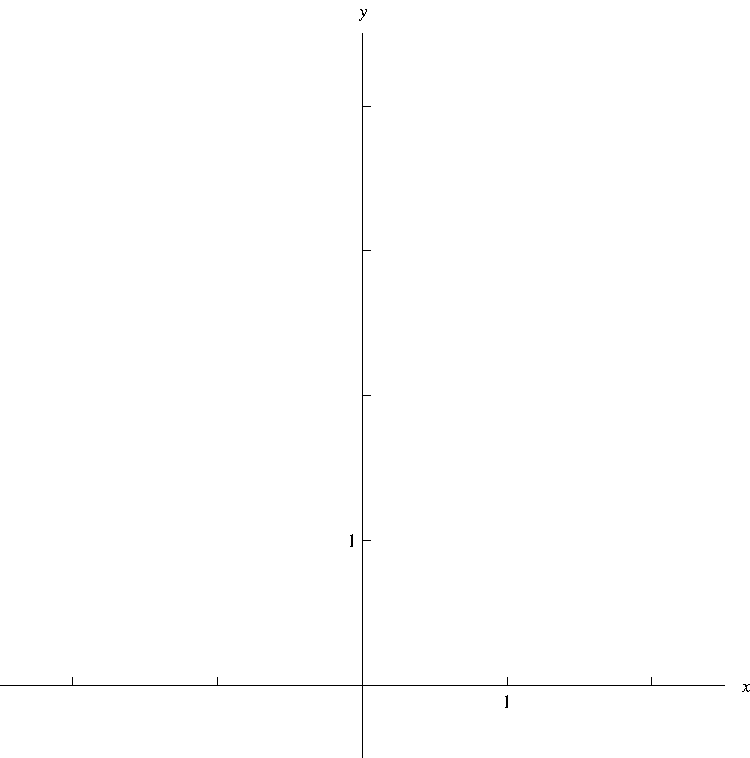
\includegraphics[height=6cm]{exponential-functions/pictures/twoxa.pdf}%
%}%
%\only<handout:0| 3-4>{%
%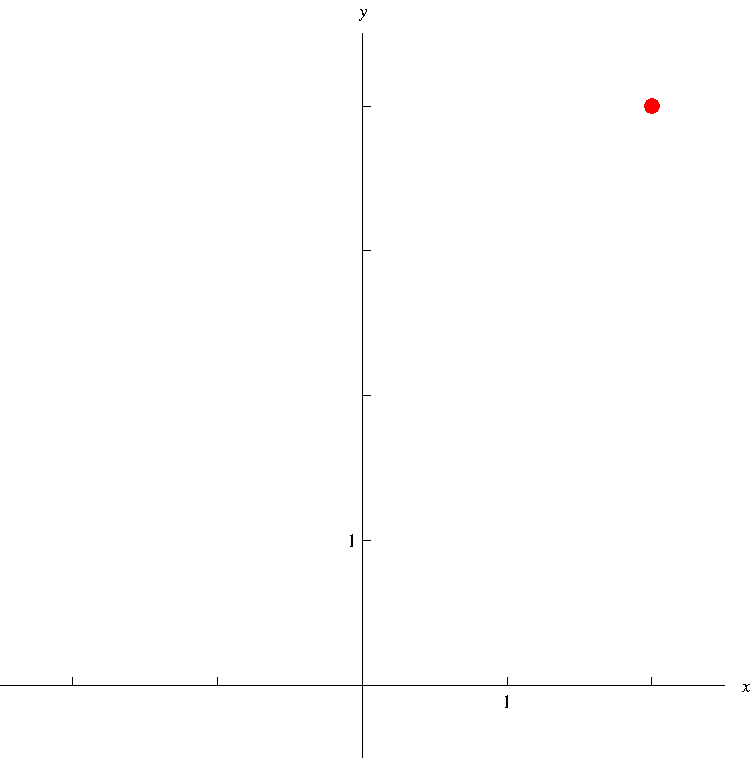
\includegraphics[height=6cm]{exponential-functions/pictures/twoxb.pdf}%
%}%
%\only<handout:0| 5-6>{%
%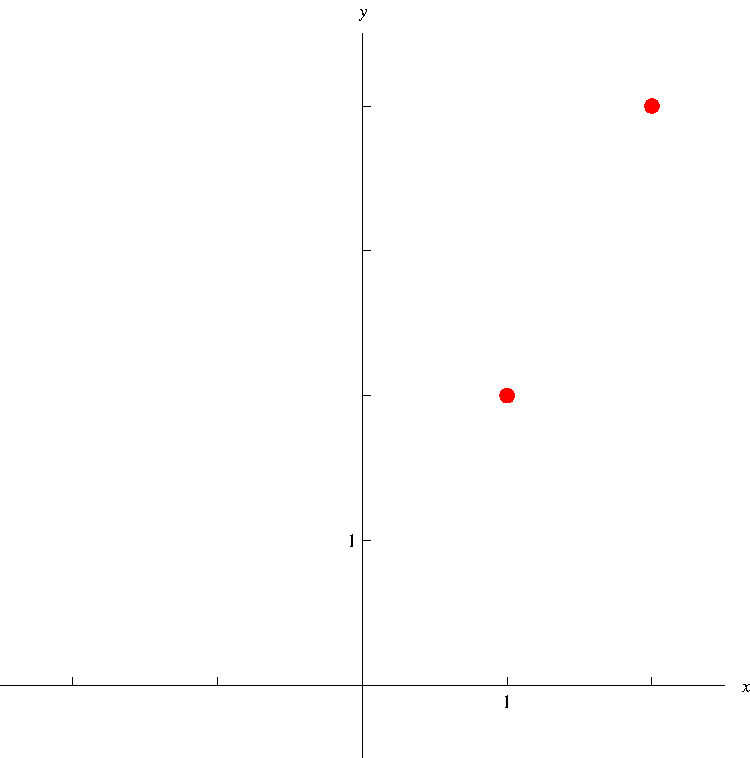
\includegraphics[height=6cm]{exponential-functions/pictures/twoxc.pdf}%
%}%
%\only<handout:0| 7-8>{%
%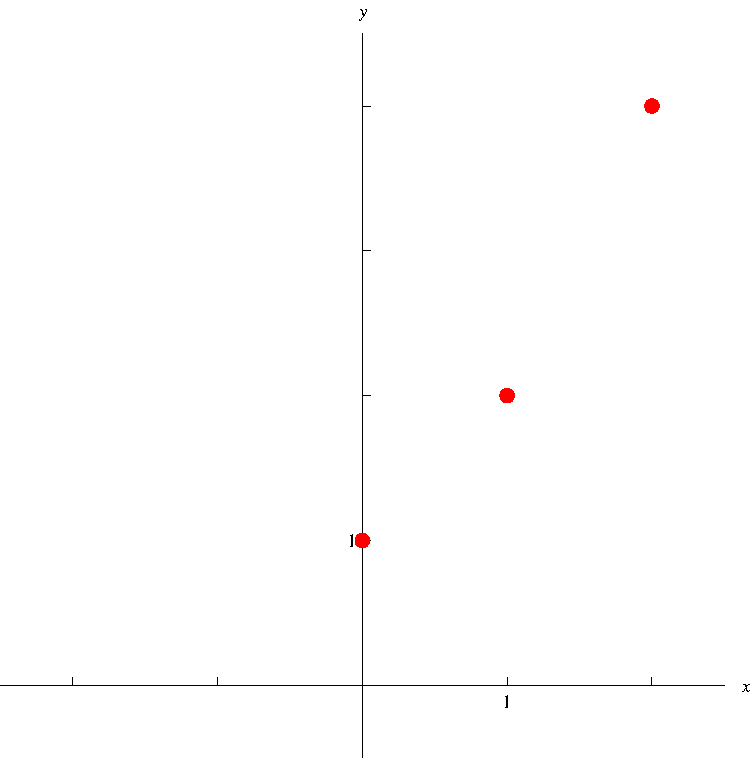
\includegraphics[height=6cm]{exponential-functions/pictures/twoxd.pdf}%
%}%
%\only<handout:0| 9-10>{%
%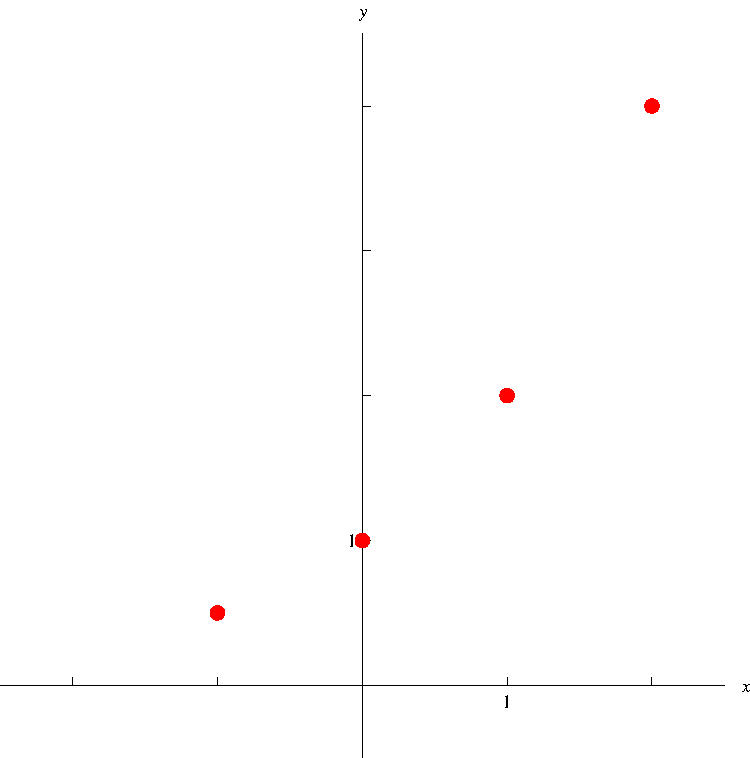
\includegraphics[height=6cm]{exponential-functions/pictures/twoxe.pdf}%
%}%
%\only<handout:0| 11>{%
%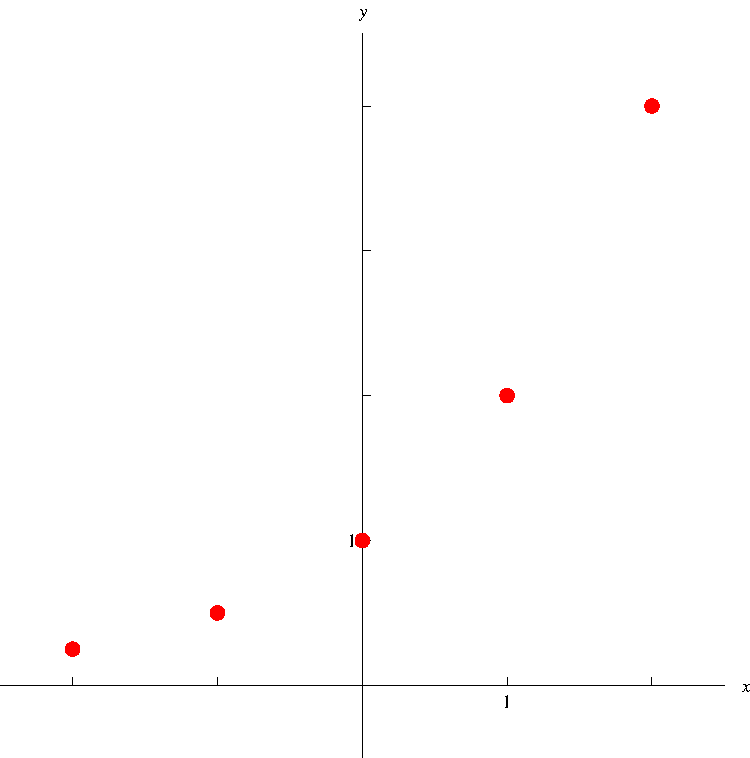
\includegraphics[height=6cm]{exponential-functions/pictures/twoxf.pdf}%
%}%
%\only<handout:1| 12->{%
%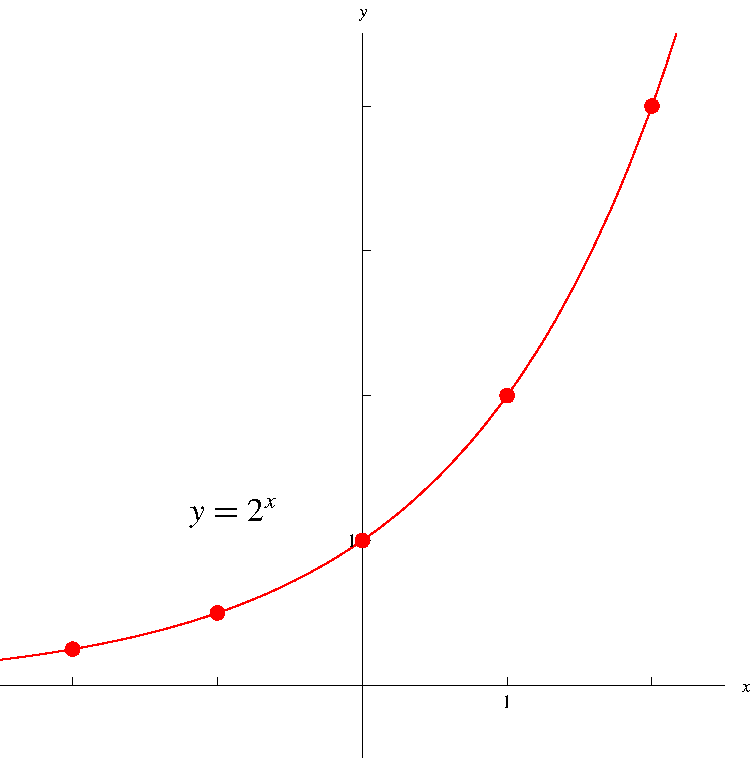
\includegraphics[height=6cm]{exponential-functions/pictures/twoxg.pdf}%
%}%


\column{.5\textwidth}
\[
\begin{array}{r|l}
x & y\\
\hline
\alert<handout:0| 2-3>{2} & \alert<handout:0| 3>{\uncover<3->{4}} \\
\alert<handout:0| 4-5>{1} & \alert<handout:0| 5>{\uncover<5->{2}} \\
\alert<handout:0| 6-7>{0} & \alert<handout:0| 7>{\uncover<7->{1}} \\
\alert<handout:0| 8-9>{-1} & \alert<handout:0| 9>{\uncover<9->{1/2}} \\
\alert<handout:0| 10-11>{-2} & \alert<handout:0| 11>{\uncover<11->{1/4}} 
\end{array}
\]
\uncover<13->{
\begin{definition}[Exponential Function]
An exponential function is a function of the form $f(x) = a^x$, where $a$ is a positive constant.
\end{definition}
}
\end{columns}
\end{frame}
% end module exponential-function-def
% begin module exponential-function-graphs-plus
\begin{frame}
\begin{columns}
\column{0.7\textwidth}
Graphs of various exponential functions.

\psset{xunit=2cm, yunit=2cm}
\begin{pspicture}(-2.1,-0.2)(2.2,3.6) 
\psframe*[linecolor=white](-2.1,-0.2)(2.1,3.5)
\psaxes[labels=none]{<->}(0,0)(-2.1,-0.2)(2.1,3.5)
\uncover<1->{
\rput[r](1.8, 2.3){$y=2^x$}
%Function formula: 2^{x} 
\psplot[linecolor=red, plotpoints=1000]{-2}{1.584962501}{2 x exp }
}
\uncover<2->{
\rput[l](0.7, 3.1){$y=4^x$}
%Function formula: 4^{x} 
\psplot[linecolor=black, plotpoints=1000]{-2}{0.79248125}{4 x exp }
}
\uncover<3->{
\rput[b](0.4, 3.05){$y=10^x$}
%Function formula: 4^{x} 
\psplot[linecolor=blue, plotpoints=1000]{-2}{0.477121255}{10 x exp }
}
\uncover<4->{
\rput[l](1.15, 1.5){$y=1.5^x$}
%Function formula: 4^{x} 
\psplot[linecolor=green, plotpoints=1000]{-2}{2}{1.5 x exp }
}
\uncover<5->{
\rput[l](-1.9, 2){$y=0.5^x$}
%Function formula: 4^{x} 
\psplot[linecolor=purple, plotpoints=1000]{-1.584962501}{2}{0.5 x exp }
}
\uncover<6->{
\rput[l](-1.2, 3.1){$y=0.25^x$}
%Function formula: 4^{x} 
\psplot[linecolor=brown, plotpoints=1000]{-0.79248125}{2}{0.25 x exp }
}
\end{pspicture}

\column{0.3\textwidth}
\uncover<7->{Observations}
 
\begin{itemize}
\item<8-| alert@8-9> $a^x$ is always \uncover<9->{positive.}  
\item<10-| alert@10-11> $a^0 = \uncover<11->{1}$ for all $a$.  
\end{itemize}
\uncover<12->{$a > 1$:}
\begin{itemize}
\item<12-| alert@12-13> $\displaystyle \lim_{x\to\infty}a^x = \uncover<13->{\infty.}$
\item<12-| alert@14-15> $\displaystyle \lim_{x\to-\infty}a^x = \uncover<15->{0.}$
\end{itemize}
\uncover<12->{$a < 1$:}
\begin{itemize}
\item<12-| alert@16-17> $\displaystyle \lim_{x\to\infty}a^x = \uncover<17->{0.}$
\item<12-| alert@18-19> $\displaystyle \lim_{x\to-\infty}a^x = \uncover<19->{\infty.}$
\end{itemize}
\end{columns}

\end{frame}
% end module exponential-function-graphs-plus

% begin module exponential-properties
\begin{frame}[t]
Properties of exponential expressions.  

\uncover<8->{Suppose $a$ is positive.  Then}
\begin{enumerate}
\item<8->  $a^xa^y = a^{x+y}$
\item<15->  $\frac{a^x}{a^y} = a^{x-y}$
\item<20->  $(a^x)^y = a^{xy}$
\item<28->  $(ab)^x = a^xb^x$
\end{enumerate}

\only<-8| handout:0>{%
\begin{align*}
\uncover<2->{\alert<2-3>{2^3}\cdot \alert<4-5>{2^2} & = \alert<2-3>{(\uncover<3->{2\cdot 2\cdot 2})}\alert<4-5>{(\uncover<5->{2\cdot 2})} } \\
\uncover<6->{ & = 2\cdot 2\cdot 2\cdot 2\cdot 2 } \\
\uncover<7->{ & = 2^5.}
\end{align*}
}%

\only<9-15| handout:0>{%
\begin{align*}
\uncover<9->{\frac{\alert<9-10>{2^3}}{\alert<11-12>{2^2}} & = \frac{\alert<9-10>{\uncover<10->{\alert<13>{2\cdot 2}\cdot 2}}}{\alert<11-13>{\uncover<12->{2\cdot 2}}} } \\
\uncover<13->{ & = 2 } \\
\uncover<14->{ & = 2^1.}
\end{align*}
}%

\only<16-20| handout:0>{%
\begin{align*}
\uncover<16->{(2^2)^4 & = 2^2\cdot 2^2\cdot2^2\cdot 2^2 } \\
\uncover<17->{ & = (2\cdot 2)(2\cdot 2)(2\cdot 2)(2\cdot 2) } \\
\uncover<18->{ & = 2\cdot2\cdot2\cdot2\cdot2\cdot2\cdot2\cdot2 } \\
\uncover<19->{ & = 2^8 } 
\end{align*}
}%

\only<21-28| handout:0>{%
\begin{align*}
\uncover<21->{(2\cdot 3)^3 & = (2\cdot 3)(2\cdot 3)(2\cdot 3) } \\
\uncover<22->{ & = 2\cdot 3 \cdot 2\cdot 3 \cdot 2\cdot 3 } \\
\uncover<23->{ & = \alert<24-25>{2\cdot 2 \cdot 2}\cdot \alert<26-27>{3 \cdot 3\cdot 3} } \\
\uncover<24->{ & = \alert<24-25>{\uncover<25->{2^3}} \cdot \alert<26-27>{\uncover<27->{3^3}} } 
\end{align*}
}%

\end{frame}
% end module exponential-properties

% begin module exponential-equation1
\begin{frame}
\begin{example}[Solving an exponential equation]
Solve for $t$.  
\begin{align*}
16^{4t} & = 8^{t-2} \\
\uncover<2->{\text{Find a common base:}\quad \alert<2-3>{\big( \uncover<3->{2^4}\big)}^{4t}} & \uncover<2->{ = \alert<2-3>{\big( \uncover<3->{2^3}\big)}^{t-2} } \\
\uncover<4->{2^{16t}} & \uncover<4->{ = 2^{3t-6}} \\
\uncover<5->{16t} & \uncover<5->{ = 3t - 6} \\
\uncover<6->{13t} & \uncover<6->{ =  -6} \\
\uncover<7->{t} & \uncover<7->{ =  -6/13.} 
\end{align*}
\end{example}
\end{frame}
% end module exponential-equation1

% begin module exponential-word-problem1
\begin{frame}
\begin{example}[Solving an exponential word problem]
A farmer buys \alert<handout:0| 8>{$48$ chickens} and \alert<handout:0| 10>{$6$ rabbits}.
\alert<handout:0| 8>{The chicken population doubles each year}, and \alert<handout:0| 10>{the rabbit population doubles every six months.}
\alert<handout:0| 3>{When} does the farmer have \alert<handout:0| 5>{the same} \alert<handout:0| 4,6>{number of} \alert<handout:0| 4>{chickens} as \alert<handout:0| 6>{rabbits}?

\uncover<2->{%
Let $c(t)$ denote the number of chickens after $t$ years, and let $r(t)$ denote the number of rabbits after $t$ years.
}%
\abovedisplayskip=0pt
\belowdisplayskip=0pt
\begin{align*}
\uncover<3->{\alert<3| handout:0>{\text{Solve for $t$:}}}\quad  \uncover<4-| handout:0>{\alertNoH{4,7-8}{c(t)}} & \uncover<5->{\alert<5| handout:0>{=}} \uncover<6-| handout:0>{\alertNoH{6,9-10}{r(t)}} \\
\uncover<8-| handout:0>{\alertNoH{8}{\alertNoH{11}{48}\cdot 2^t}} & \uncover<7->{=} \uncover<10-| handout:0>{\alertNoH{10}{\alertNoH{11}{6}\cdot 4^t}} \\
\uncover<11-| handout:0>{\alertNoH{11-13}{8}\cdot 2^t} & \uncover<11->{=} \uncover<11-| handout:0>{\alertNoH{14-15}{4^t}} \\
\uncover<12-| handout:0>{\text{Find a common base:}\quad \alertNoH{12-13}{2^{\uncover<13->{3}}}\cdot 2^t } & \uncover<12->{=} \uncover<12-| handout:0>{\alertNoH{14-15}{2^{\uncover<15->{2t}}}} \\
\uncover<16-| handout:0>{2^{t+3}} & \uncover<16->{=} \uncover<16-| handout:0>{2^{2t}} \\
\uncover<17-| handout:0>{t+3} & \uncover<17->{=} \uncover<17-| handout:0>{2t} \\
\uncover<18->{t} & \uncover<18->{=} \uncover<18-| handout:0>{3.}
\end{align*}
\uncover<19-| handout:0>{Therefore the chicken and rabbit populations are equal after $3$ years.}
\end{example}
\end{frame}
% end module exponential-word-problem1

% begin module exponential-equation2
\begin{frame}
\begin{example}[Solving a quadratic exponential equation]
Solve for $x$.  
\abovedisplayskip=0pt
\belowdisplayskip=0pt
\begin{align*}
9^x & = 2\cdot 3^x + 63 \\
\uncover<2-| handout:0>{\alert<handout:0| 4-5>{9^x} -2\cdot \alert<handout:0| 3>{3^x} - 63} & \uncover<2->{ = 0} \\
\intertext{\uncover<3->{Substitute $\alert<handout:0| 9>{u = \uncover<3-| handout:0>{3^x}}$:}}
\uncover<3-| handout:0>{\alert<handout:0| 4-5>{\uncover<5->{u^2}} - 2\alert<handout:0| 3>{u} - 63} & \uncover<3->{ = 0} \\
\uncover<6->{\alert<handout:0| 6-7>{(\uncover<7-| handout:0>{u-9})(\uncover<7-| handout:0>{u+7})}} & \uncover<6->{ = 0 } 
\end{align*}
\begin{align*}
\uncover<8->{ \alert<handout:0| 9>{u} } & \uncover<8->{ = \uncover<8-| handout:0>{9} } & \uncover<8->{\text{or}} & & \uncover<8->{\alert<handout:0| 9>{u}} & \uncover<8->{ = \uncover<8-| handout:0>{-7}} \\
\uncover<9-| handout:0>{ \alert<handout:0| 9>{3^x} } & \uncover<9-| handout:0>{ = 9 } & \uncover<9-| handout:0>{\text{or}} & & \uncover<9-| handout:0>{\alert<handout:0| 9>{3^x}} & \uncover<9-| handout:0>{ = -7} \invisible{99999999} \\
\uncover<10-| handout:0>{ \alert<handout:0| 10-11>{x} } & \uncover<10-| handout:0>{ \alert<handout:0| 10-11>{ = \uncover<11->{2} }} & & & \uncover<10-| handout:0>{\alert<handout:0| 12-13>{\uncover<-12>{x}}} & \uncover<10-| handout:0>{ \alert<handout:0| 12-13>{ \only<-12>{ =} \only<13->{\text{no solution}} }} 
\end{align*}
\uncover<14-| handout:0>{Therefore $x = 2$ is the solution.}
\end{example}
\end{frame}
% end module exponential-equation2

% end lecture

% begin lecture
\lect{February 14, 2014}{Lecture  6}{6}
\section{Exponential Functions}
\subsection{The Natural Exponential Function}
% begin module exponential-function-derivative
\begin{frame}
\frametitle{Derivatives of Exponential Functions}
Compute the derivative of $f(x) = a^x$ using the definition:
\begin{align*}
\uncover<2->{f'(x) = \lim_{h\to 0} \frac{f(x+h)-f(x)}{h}} & \uncover<3->{=}  \uncover<3->{\lim_{h\to 0} \frac{\alert<handout:0| 4>{a^{x+h}}-a^x}{h}}\\
 & \uncover<4->{=}  \uncover<4->{\lim_{h\to 0} \frac{\alert<handout:0| 5>{\alert<handout:0| 4>{a^x a^h}-a^x}}{h}}\\
 & \uncover<5->{=}  \uncover<5->{\lim_{h\to 0} \frac{\alert<handout:0| 5>{\alert<handout:0| 6>{a^x} (a^h- 1)}}{h}}\\
 & \uncover<6->{=}  \uncover<6->{\alert<handout:0| 6>{a^x} \alert<handout:0| 7>{\lim_{h\to 0} \frac{a^h- 1}{h}}}\\
 & \uncover<7->{=}  \uncover<7->{a^x \alert<handout:0| 7>{f'(0)}.}
\end{align*}
\end{frame}


\begin{frame}
We have shown that, if $f(x) = a^x$ is differentiable at 0, then it is differentiable everywhere, and
\[
f'(x) = f'(0)a^x .
\]
\uncover<2->{
We leave the following theorem without proof. 
\begin{theorem}
Let $a$ be a positive number and let $f(x)=a^x$. Then the limit \[f'(0)=\lim_{h\rightarrow 0}\frac{a^h - 1}{h}\] exists. 
\end{theorem}

In fact, it can be shown, as was/will be done in Calculus I that the limit above equals $\ln a$, i.e., $f'(0)=\ln(a)$. Here, $\ln$ is the natural logarithm function (was/will be defined in Calculus I).
}
\end{frame}
% end module exponential-function-derivative

% begin module e-def
\begin{frame}
\[
\text{If}\quad  f(x) = a^x, \quad \text{then}\quad f'(x) = f'(0)a^x .
\]
The simplest differential formula occurs when $f'(0) = 1$.  Since $\lim_{h\rightarrow 0}\frac{2^h-1}{h}\approx 0.69$ and $\lim_{h\rightarrow 0}\frac{3^h-1}{h}\approx 1.10$, we expect there is a number $a$ between 2 and 3 such that $\lim_{h\rightarrow 0}\frac{a^h-1}{h} = 1$.  
\uncover<2->{
\begin{definition}[$e$]
$e$ is the number such that $\lim_{h\rightarrow 0}\frac{e^h-1}{h} = 1$.
\end{definition}
}

\begin{columns}
\column{.3\textwidth}
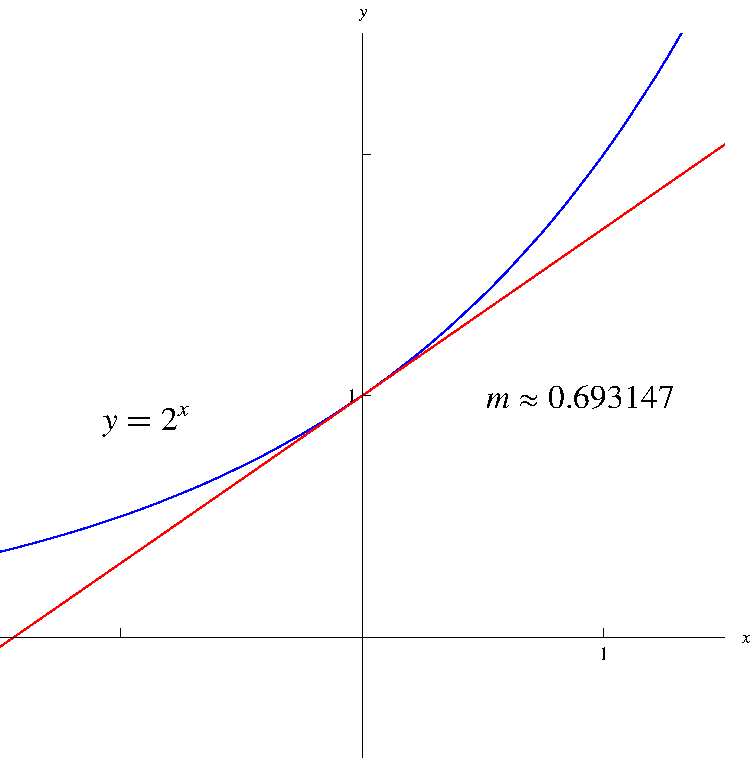
\includegraphics[height=4cm]{exponential-functions/pictures/exp-tangent-two.pdf}%
\column{.3\textwidth}
\uncover<handout: 1|3->{%
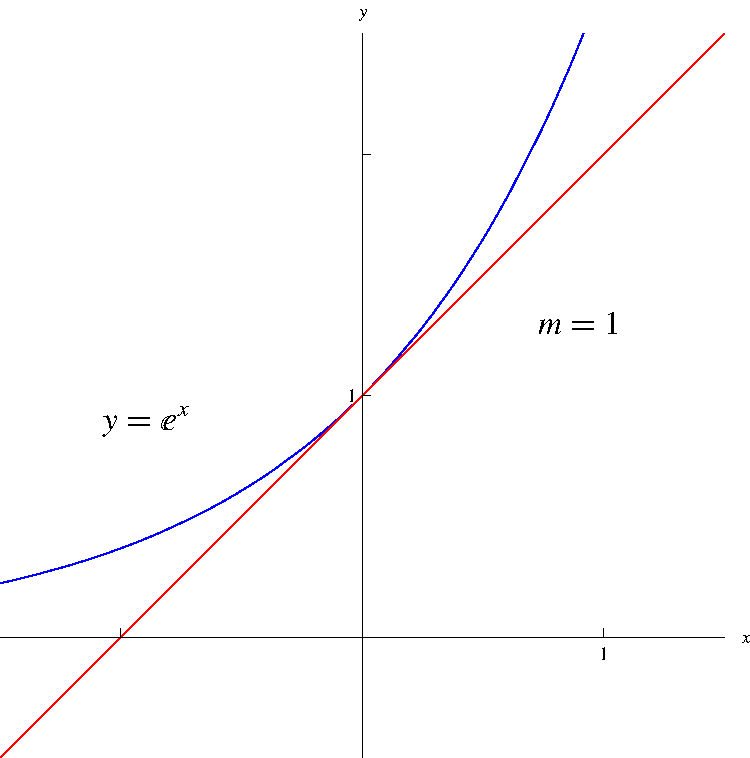
\includegraphics[height=4cm]{exponential-functions/pictures/exp-tangent-e.pdf}%
}%
\column{.3\textwidth}
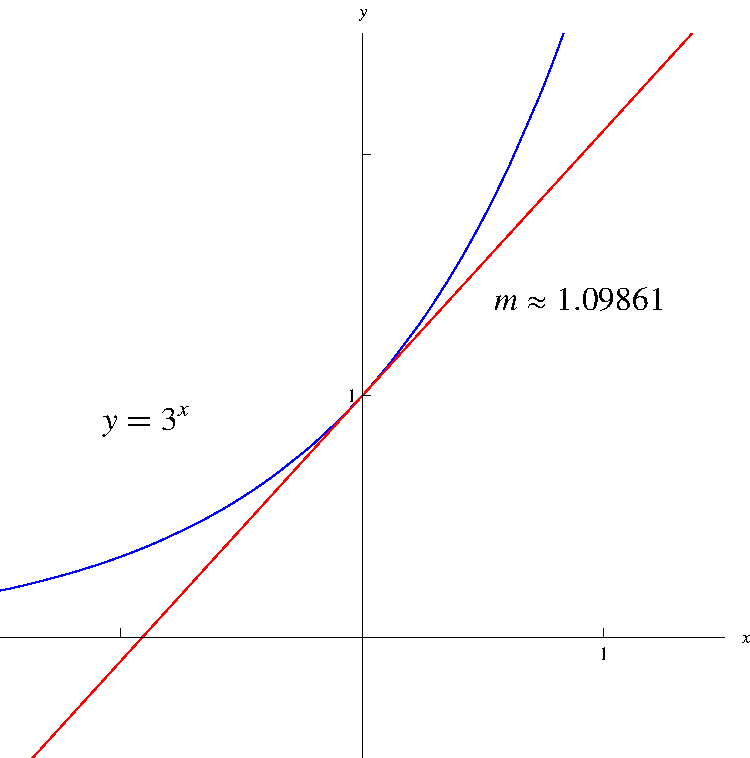
\includegraphics[height=4cm]{exponential-functions/pictures/exp-tangent-three.pdf}%
\end{columns}
\end{frame}
% end module e-def

% begin module natural-exponential-def
\begin{frame}
\begin{definition}[Natural Exponential Function]
$e^x$ is called the natural exponential function.  Its derivative is
\[
\frac{\diff}{\diff x} e^x = e^x .
\]
\end{definition}
\uncover<2->{
We can use this fact to find an approximation for $e$:
}
\begin{itemize}
\item<3->  Let $\alert<handout:0| 7,12>{e = 2^c}$.
\item<4->  Let $f(x) = 2^x$.  Then $\alert<handout:0| 8>{f'(x) = k2^x}$, where $\alert<handout:0| 13>{k = f'(0) \approx 0.693147}$.
\item<5->  $\alert<handout:0| 6>{e^x = \uncover<6->{\frac{\diff}{\diff x} (\alert<handout:0| 7>{e^x})}} \uncover<7->{ = \alert<handout:0| 8>{\frac{\diff}{\diff x} (\alert<handout:0| 7>{2^{cx}})}} \uncover<8->{\alert<handout:0| 8>{= k2^{cx}\frac{\diff}{\diff x} (cx) }} \uncover<9->{= ck 2^{cx}.}$
\item<10->  Substitute $x = 0$: $1 = e^0 = ck2^0 = ck$.
\item<11->  Therefore $\alert<handout:0| 12>{c = 1/k}$.
\item<12->  $\alert<handout:0| 12>{e = 2^{1/\alert<handout:0| 13>{k}}} \uncover<13->{ \approx 2^{1/\alert<handout:0| 13>{0.693147}}} \uncover<14->{\approx 2.71828 .}$
\end{itemize}
\end{frame}
% end module natural-exponential-def

% begin module derivative-e-plus-polynomial
\begin{frame}
\begin{example}[Derivative of a Polynomial and the Natural Exponential Function]
\abovedisplayskip=0pt
\belowdisplayskip=-15pt
\abovedisplayshortskip=0pt
\belowdisplayshortskip=0pt
\begin{align*}
\text{Differentiate}\quad y & = e^x+x^7.\\
\uncover<2->{\frac{\diff y}{\diff x} & = \frac{\diff}{\diff y}(\alert<3-4>{e^x}) + \frac{\diff}{\diff y}(\alert<5-6>{x^7})}\\
& \uncover<3->{= \uncover<4->{\alert<4>{e^x}}  + \uncover<6->{\alert<6>{7x^6}.}}
\end{align*}
\end{example}
\end{frame}
% end module derivative-e-plus-polynomial
% begin module chain-rule-e
\begin{frame}
\chainruley{e^{-3x}}{-3x}{e^{u}}{e^{UU}}{-3}{-3e^{UU}}{Natural Exponential Function}
\end{frame}
% end module chain-rule-e

% begin module chain-rule-twice-ex2
\begin{frame}
\chainruletwice%
{ e^{\tan \left(\pi x\right)}}%
{e^{\tan \left(\pi x\right)}}%
{\tan\left(\pi x\right)}%
{\sec^2 \left(\pi x\right)}%
{\pi x}%
{\pi}%
{}%
{\pi e^{\tan \left(\pi x\right)}\sec^2 \left(\pi x\right)}%
{}%
\end{frame}
% end module chain-rule-twice-ex2

\section{Inverse Functions}
\subsection{One-to-one Functions}
% begin module one-to-one-def
\begin{frame}
\frametitle{One-to-one Functions}
\begin{definition}[One-to-one Function]
A function $f$ is a one-to-one function if it never takes on the same value twice; that is,
\[
f(x_1) \neq f(x_2) \ \text{whenever }  \ x_1 \neq x_2 .
\]
\end{definition}
\begin{columns}[c]
\column{.5\textwidth}
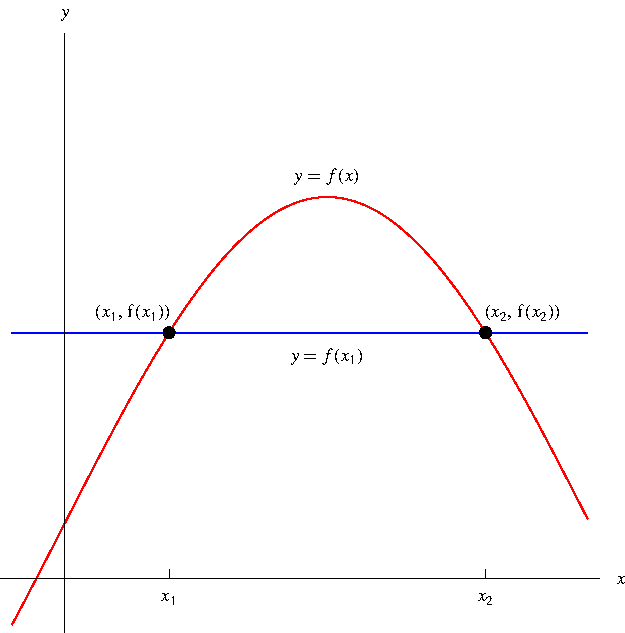
\includegraphics[height=5cm]{inverse-functions/pictures/07-01-1-1def.pdf}%
\column{.5\textwidth}
$\leftarrow$ This function is not one-to-one.
\end{columns}
\end{frame}
% end module one-to-one-def

% begin module horizontal-line-test
\begin{frame}
Question: How can we tell from the graph of a function whether it is one-to-one or not?

Answer: Use the horizontal line test.

\begin{proof}[The Horizontal Line Test]
A function is one-to-one if and only if no horizontal line intersects it more than once.
\end{proof}

\begin{tabular}{cc}
\psset{xunit=0.7cm, yunit=0.7cm}
\begin{pspicture}(-5, -5)(5,5) 
\psframe*[linecolor=white](-5,-5)(5,5) 
\psaxes[ticks=none, labels=none]{<->}(0,0)(-3,-3)(3,3)
%Function formula: 1/2 (x)+1/2 
\psplot[linecolor=red, plotpoints=1000]{1}{2}{0.5 x 0.5 mul add } %Function formula: (x)^{3} 
\psplot[linecolor=red, plotpoints=1000]{-1}{1}{x 3 exp } %Function formula: 3/2 (x)+1/2 
\psplot[linecolor=red, plotpoints=1000]{-2}{-1}{0.5 x 1.5 mul add }
\end{pspicture} 
%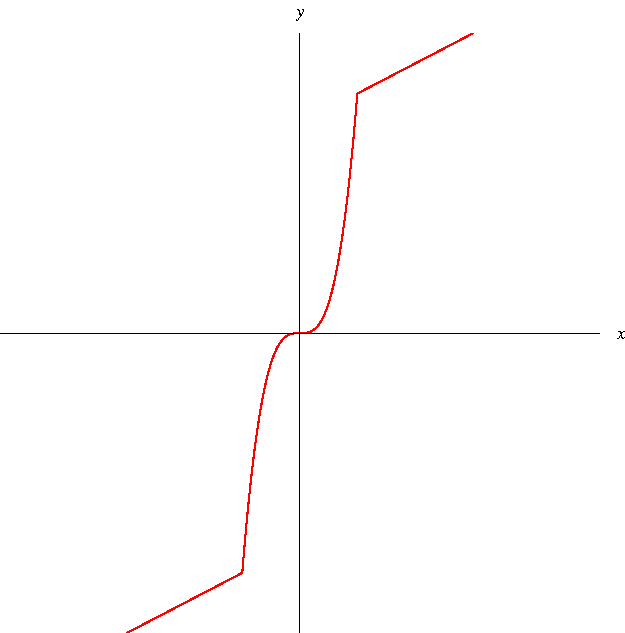
\includegraphics[height=4cm]{inverse-functions/pictures/07-01-onetoone.pdf} 
 %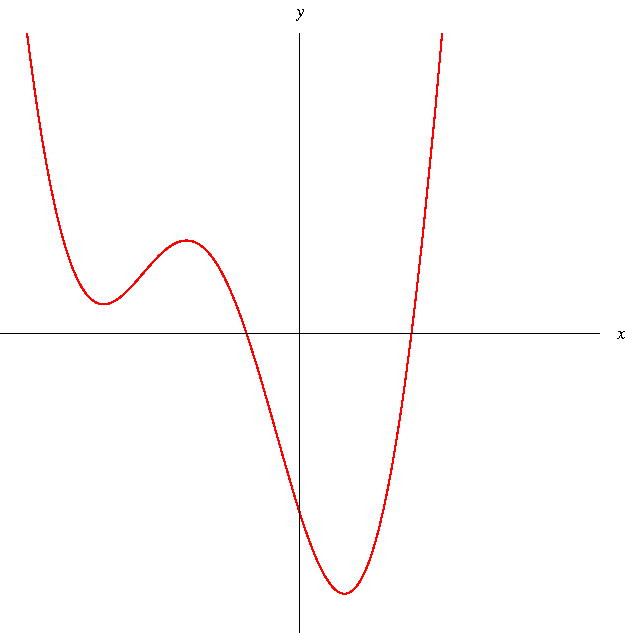
\includegraphics[height=4cm]{inverse-functions/pictures/07-01-notonetoonea.pdf}%
&%
\uncover<handout:0| 2->{%
\psset{xunit=0.7cm, yunit=0.7cm}
\begin{pspicture}(-5, -5)(5,5) 
\psframe*[linecolor=white](-5,-5)(5,5) 
\psaxes[ticks=none, labels=none]{<->}(0,0)(-3,-3)(3,3)
 %Function formula: -2/5+((6/5+x)^{2}) ((x) (x))-6/25 ((6/5+x)^{2})- (((6/5+x)^{2}) (x)) 
 \psplot[linecolor=red, plotpoints=1000]{-2}{1.5}{x x 1.2 add 2 exp mul -1 mul x 1.2 add 2 exp -0.24 mul add x x mul x 1.2 add 2 exp mul add -0.4 add }
 \uncover<3->{
 \psline[linestyle=dashed](-3, 1)(3, 1)
 }
 \end{pspicture} 
}
\\
\uncover<2->{\alert<handout:0| 2>{One-to-one}} &
\uncover<3->{\alert<handout:0| 3>{Not one-to-one}}
\end{tabular}
\end{frame}
% end module horizontal-line-test

\subsection{The Definition of the Inverse of $f$}
% begin module inverse-function-def
\begin{frame}
\frametitle{The Definition of the Inverse of $f$}
\begin{definition}[$f^{-1}$]
Let $f$ be a one-to-one function with domain $A$ and range $B$.  Then the inverse of $f$ is the function $f^{-1}$ that has domain $B$ and range $A$ and is defined by
\[
f^{-1}(y) = x \qquad \Leftrightarrow \qquad f(x) = y 
\]
for all $y$ in $B$.
\end{definition}
\begin{columns}[T]
\column{.5\textwidth}
\uncover<2->{Note:}
\begin{itemize}
\item<3->  Only one-to-one functions have inverses.
\item<4->  $f^{-1}$ reverses the effect of $f$.
\item<5->  domain of $f^{-1} = $ range of $f$.
\item<5->  range of $f^{-1} = $ domain of $f$.
\end{itemize}
\column{.5\textwidth}
\uncover<6->{
\begin{example}[$f(x) = x^3$]
The inverse of $f(x) = x^3$ is $f^{-1}(x) = \sqrt[3]{x}$.  This is because if $y = x^3$, then
\[
f^{-1}(y) = \sqrt[3]{y} = \sqrt[3]{x^3} = x .
\]
\end{example}
}
\end{columns}
\end{frame}
% end module inverse-function-def

% begin module inverse-notation-warning
\begin{frame}
\alert<1->{WARNING:}

Do not mistake the $-1$ in $f^{-1}(x)$ for an exponent.
\[
f^{-1}(x) \ \text{does not mean } \ \frac{1}{f(x)} .
\]

If you want to write $\frac{1}{f(x)}$ using exponents, you can write $(f(x))^{-1}$.
\begin{itemize}
\item<2->  $f^{-1}(x)$ is the compositional inverse of $f$.
\item<3->  $\frac{1}{f(x)}$ is the multiplicative inverse of $f$.
\end{itemize}
\end{frame}
% end module inverse-notation-warning

% begin module inverse-function-solve-for
\begin{frame}
\frametitle{How to Find the Inverse of a One-to-one Function}
\begin{enumerate}
\item<1-| alert@3>  Write $y = f(x)$.
\item<1-| alert@4-5>  Solve this equation for $x$ in terms of $y$ (if possible).
\item<1-| alert@6>  Interchange $x$ and $y$.  The resulting equation is $y = f^{-1}(x)$. 
\end{enumerate}
\uncover<2->{
\begin{example}%[Example 4, p. 388]
If $f(x) = x^3 + 2$, find a formula for $f^{-1}(x)$.
\begin{align*}
\uncover<3->{y} & \uncover<3->{=}  \uncover<3->{x^3 + 2}\\
\uncover<4->{x^3} & \uncover<4->{=}  \uncover<4->{y - 2}\\
\uncover<5->{\alert<handout:0| 6>{x}} & \uncover<5->{=}  \uncover<5->{\sqrt[3]{\alert<handout:0| 6>{y} - 2}}\\% 
\uncover<6->{\alert<handout:0| 6>{y}} & \uncover<6->{=}  \uncover<6->{\sqrt[3]{\alert<handout:0| 6>{x} - 2}} \qquad \uncover<6->{\alert<handout:0| 6>{\text{(New equation.)}}}
\end{align*}
\uncover<7->{
Therefore $f^{-1}(x) = \sqrt[3]{x - 2}$.
}
\end{example}
}
\end{frame}
% end module inverse-function-solve-for

% end lecture

% begin lecture
\lect{February 21, 2014}{Lecture  8}{8}
\section{Inverse Functions}
\subsection{The Definition of the Inverse of $f$}
% begin module guess-and-check
\begin{frame}
\begin{example}[Guess and Check]
If $f(x) = 2x + \sin 2x + e^{x/2}$, find $f^{-1}(1)$.  
\begin{align*}
\uncover<2->{f\alert<handout:0| 2-3>{(\uncover<3->{0})}} & \uncover<2->{=}  \uncover<2->{2\alert<handout:0| 2-3>{(\uncover<3->{0})}  + \sin 2\alert<handout:0| 2-3>{(\uncover<3->{0})}  + e^{\alert<handout:0| 2-3>{(\uncover<3->{0})}/2} }\\ 
 & \uncover<2->{=}  \uncover<3->{0 + 0 + 1} \\
 & \uncover<2->{=}  \uncover<2->{1.} \\
\uncover<4->{\text{Therefore}\quad f^{-1}(1)} & \uncover<4->{=}  \uncover<4->{0.}
\end{align*}
\end{example}
\end{frame}
% end module guess-and-check

% begin module inverse-function-graph
\begin{frame}
\begin{tabular}{cc}
\psset{xunit=1cm, yunit=1cm}
\begin{pspicture}(-5, -5)(5,5) 
\psframe*[linecolor=white](-5,-5)(5,5) 
\psaxes[ticks=none, labels=none]{<->}(0,0)(-1.5,-1.5)(3.4,3.1)
\psLabels{3.4}{3.1}
\uncover<6->{
\psline(2.5, 1)(1, 2.5)
\psline(1.85, 1.65)(1.95, 1.75)(1.85, 1.85)
\psline(1.85, 1.85)(1.75, 1.95)(1.65, 1.85)

\psline(1.9875, 1.3125)(2.1875, 1.5125)
\psline(2.0625, 1.2375)(2.2625, 1.4375)
\psline(1.3125, 1.9875)(1.5125, 2.1875)
\psline(1.2375, 2.0625)(1.4375, 2.2625)

\psline[linecolor=blue](-1.35, -1.35)(2.8,2.8)
\rput[l](-1, -1.2){\footnotesize $y=x$}
}
\uncover<2->{
\psFullDot{2.5}{1}
\rput[lt](2.6, 1.1){\footnotesize $(a,b)$}
}
\uncover<5->{
\psFullDot{1}{2.5}
\rput[rb](0.9, 2.6){\footnotesize $(b,a)$}
}
\end{pspicture}
%\ \only<handout:0| -4>{%
%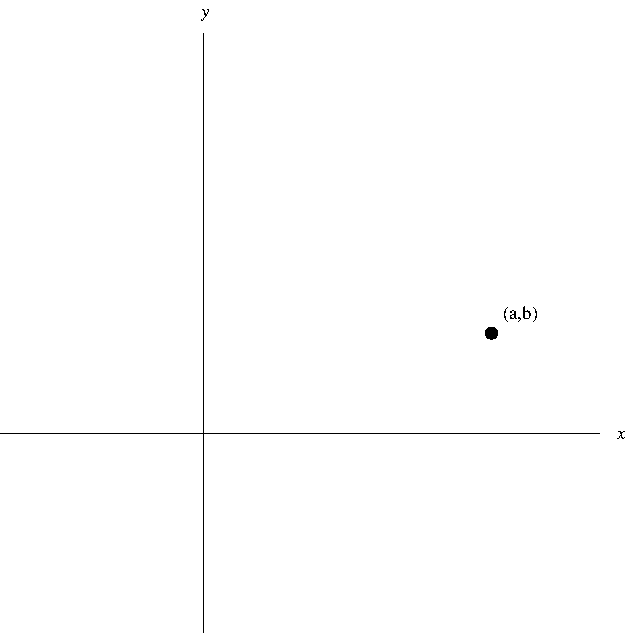
\includegraphics[height=4cm]{inverse-functions/pictures/07-01-reflecta.pdf}%
%}%
%\only<handout:0| 5>{%
%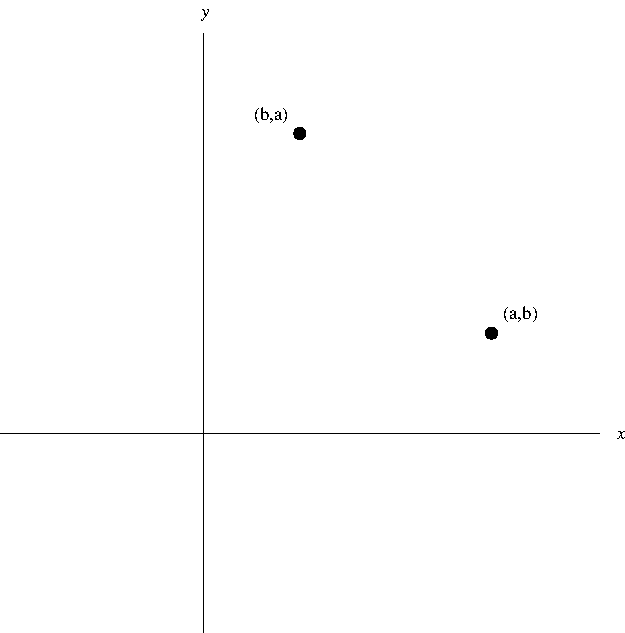
\includegraphics[height=4cm]{inverse-functions/pictures/07-01-reflectb.pdf}%
%}%
%\only<handout:1| 6->{%
%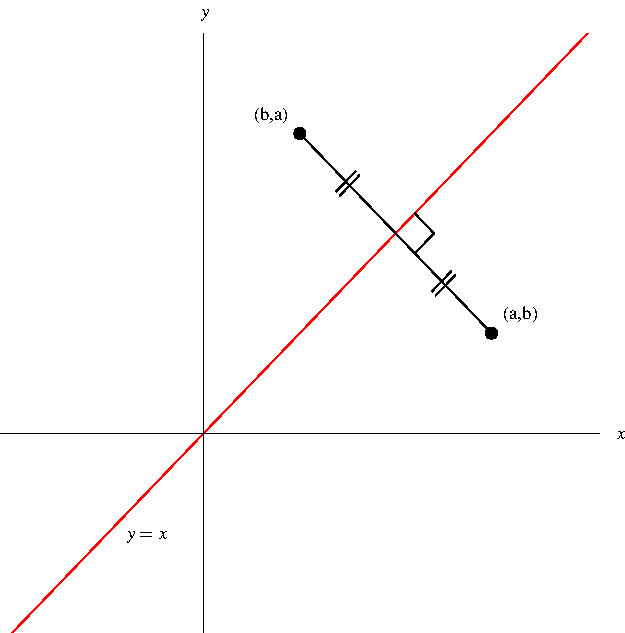
\includegraphics[height=4cm]{inverse-functions/pictures/07-01-reflectc.pdf}%
%}%
&%
\psset{xunit=1cm, yunit=1cm}
\begin{pspicture}(-5, -5)(5,5) 
\psframe*[linecolor=white](-5,-5)(5,5) 
\psaxes[ticks=none, labels=none]{<->}(0,0)(-1.55,-1.5)(3.4,3.1)
\psLabels{3.4}{3.1}
\uncover<7->{
\psline(0.75, 2.36359)(2.36359, 0.75)
\psline(1.65679, 1.65679)(1.55679, 1.75679)(1.45679, 1.65)
\psline(1.65679, 1.65679)(1.75679, 1.55679)(1.65679, 1.45679)
\psFullDot{0.75}{2.36359}
\psFullDot{2.36359}{0.75}

\psline[linecolor=blue](-1.35, -1.35)(2.8,2.8)
\rput[l](-1, -1.2){\footnotesize $y=x$}
\psplot[linecolor=red, plotpoints=1000]{-0.292893219}{3}{x 1 add ln  0.693147181 div 1 sub}
\rput[lb](0.9, 2.4){\footnotesize $y=f^{-1}(x)$}
%Function formula: 2^{1+x}-1 
\psplot[linecolor=red, plotpoints=1000]{-1.5}{0.95}{-1 2 x 1 add exp add }
\psline[linecolor=blue](-1.4, -1.4)(2.9,2.9)
\rput[l](-1, -1.2){\footnotesize $y=x$}
\rput[tr](2.8, 0.4){\footnotesize $y=f(x)$}
}
\end{pspicture} 
%\only<handout:0| -6>{%
%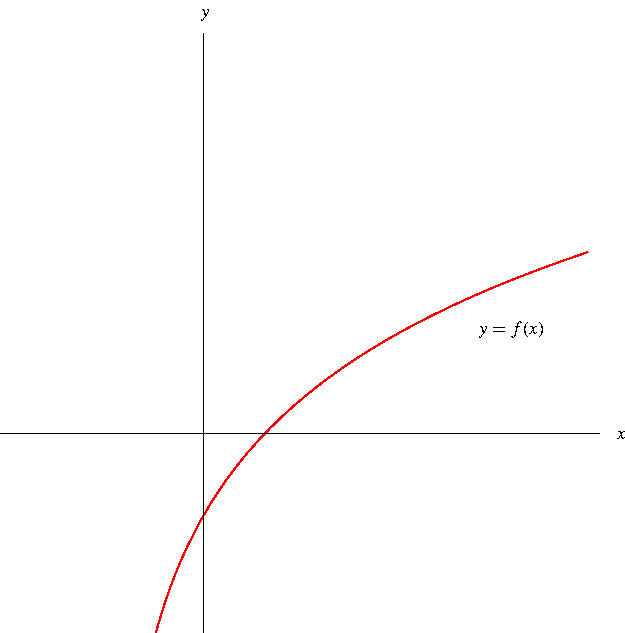
\includegraphics[height=4cm]{inverse-functions/pictures/07-01-reflect-functionb.pdf}%
%}%
%\only<handout:1| 7->{%
%\includegraphics[height=4cm]{inverse-functions/pictures/07-01-reflect-f unctiona.pdf}%
%}%
\end{tabular}

\footnotesize 
Interchanging $x$ and $y$ suggests a relation between the graphs of $f^{-1}$ and $f$:
\begin{itemize}
\item<2->  Suppose $(a,b)$ is on the graph of $f$.
\item<3->  Then $f(a) = b$.
\item<4->  Then $f^{-1}(b) = a$.
\item<5->  Then $(b,a)$ is on the graph of $f^{-1}$.
\item<6->  $(b,a)$ is the reflection of $(a,b)$ in the line $y = x$.
\item<7->  Therefore the graph of $f^{-1}$ is obtained by reflecting the graph of $f$ across the line $y = x$.
\end{itemize}
\end{frame}
% end module inverse-function-graph

% begin module inverse-function-ex5
\begin{frame}
\begin{example}%[Example 5, p. 388]
\begin{columns}[c]
\column{.5\textwidth}
\psset{xunit=0.5cm, yunit=0.5cm}
\begin{pspicture}(-5, -5)(5,5) 
\psframe*[linecolor=white](-5,-5)(5,5) \tiny
\psaxes[ticks=none, labels=none]{<->}(0,0)(-4.55,-5)(4.5,5)
\psline(1, -0.1)(1, 0.1)
\rput[t](1, -0.2){\tiny$1$}
\psline(-1, -0.1)(-1, 0.1)
\psline(-0.1, 1)(0.1, 1)
\rput[br](-0.2, 1){\tiny$1$}
\psline(-0.1, -1)(0.1, -1)
\uncover<3>{
%Function formula: sqrt{}(- (x)) 
\psplot[linecolor=red, plotpoints=1000]{-4.5}{0}{x -1 mul sqrt }
\rput(-2, 2.2){\tiny$y=\sqrt{-x}$}
}
\uncover<4->{
%Function formula: sqrt{}(- (x)) 
\psplot[linecolor=gray, plotpoints=1000]{-4.5}{0}{x -1 mul sqrt }
\rput(-2, 2.2){\color{gray}\tiny$y=\sqrt{-x}$}
}
\uncover<2>{
 %Function formula: sqrt{}(x) 
\psplot[linecolor=red, plotpoints=1000]{0}{4.5}{x sqrt } 
\rput(2.4, 1){\tiny $y=\sqrt{x}$}
}
\uncover<3->{
 %Function formula: sqrt{}(x) 
\psplot[linecolor=gray, plotpoints=1000]{0}{4.5}{x sqrt } 
\rput(2.4, 1){\color{gray}\tiny $y=\sqrt{x}$}
}
\uncover<4>{
%Function formula: sqrt{}(- (x)-1) 
\psplot[linecolor=red, plotpoints=1000]{-4.5}{-1}{-1 x -1 mul add sqrt }
\rput[r](-2.3, 0.55){\tiny$y=f(x)$}
}
\uncover<5->{
%Function formula: sqrt{}(- (x)-1) 
\psplot[linecolor=gray, plotpoints=1000]{-4.5}{-1}{-1 x -1 mul add sqrt }
\rput[r](-2.3, 0.55){\color{gray}\tiny$y=f(x)$}
}

\uncover<5>{
%Function formula: - ((x)^{2})-1 
\psplot[linecolor=red, plotpoints=1000]{0}{2}{-1 x 2 exp -1 mul add } 
\rput[l](1.3, -2){\tiny$y=f^{-1}(x)$}
\psline[linecolor=blue, linestyle=dashed] (-4.5, -4.5)(4.5, 4.5)
\rput[tl](-3, -3.2){\tiny $y=x$}
}
\end{pspicture} 
%\ \only<handout:0| -1>{%
%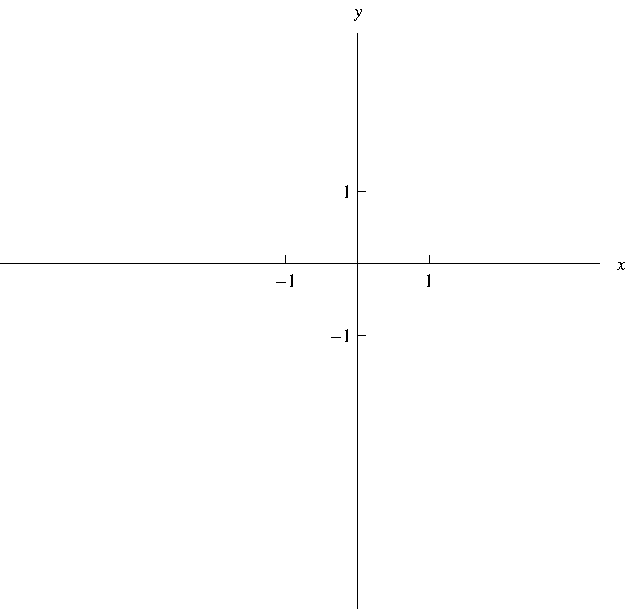
\includegraphics[height=4.5cm]{inverse-functions/pictures/07-01-ex5a.pdf}%
%}%
%\only<handout:0| 2>{%
%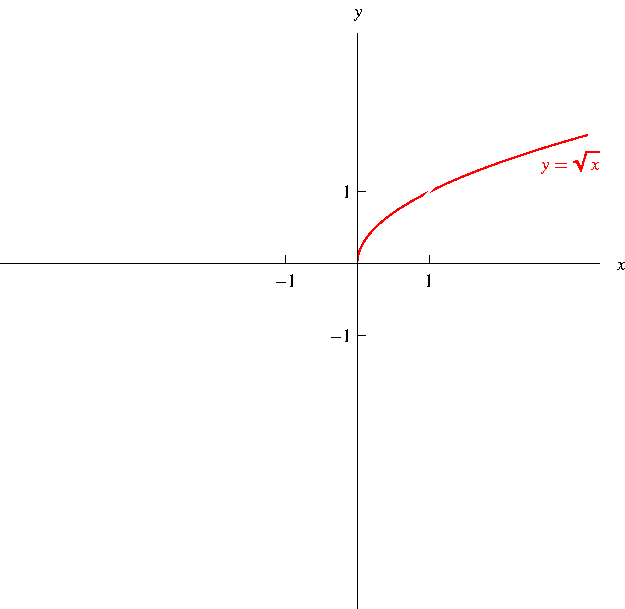
\includegraphics[height=4.5cm]{inverse-functions/pictures/07-01-ex5b.pdf}%
%}%
%\only<handout:0| 3>{%
%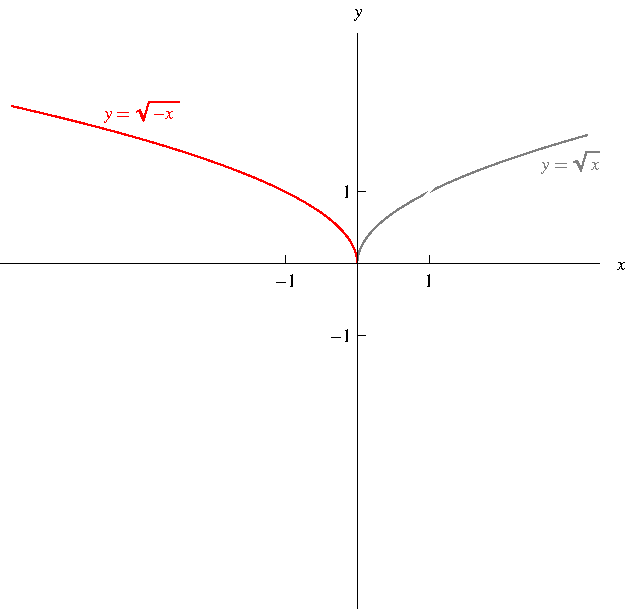
\includegraphics[height=4.5cm]{inverse-functions/pictures/07-01-ex5c.pdf}%
%}%
%\only<handout:0| 4>{%
%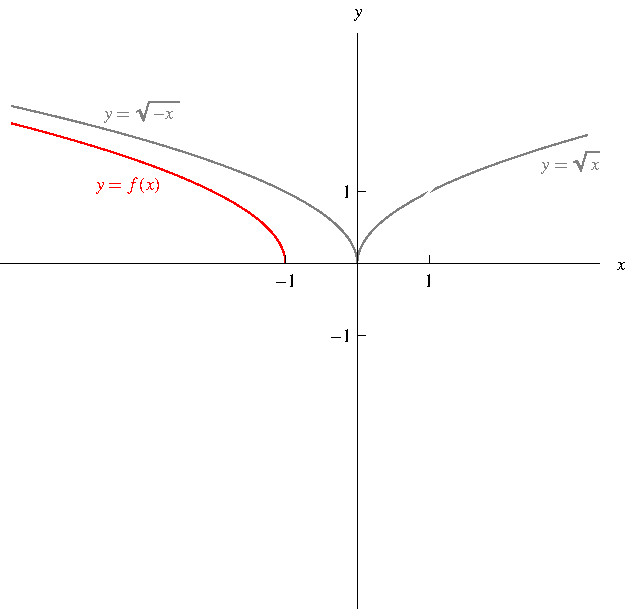
\includegraphics[height=4.5cm]{inverse-functions/pictures/07-01-ex5d.pdf}%
%}%
%\only<handout:1| 5->{%
%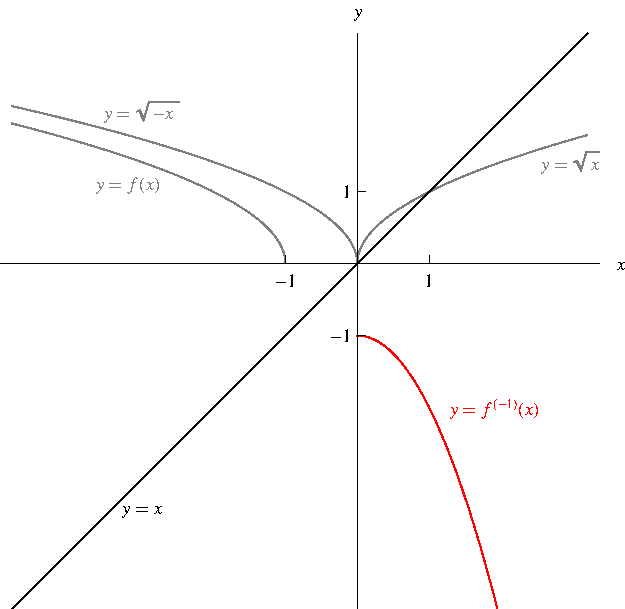
\includegraphics[height=4.5cm]{inverse-functions/pictures/07-01-ex5e.pdf}%
%}%

\column{.5\textwidth}
Sketch the graph of $f(x) = \sqrt{-x - 1}$ and its inverse function.
\end{columns}
\begin{itemize}
\item<2->  First draw the graph of $y = \sqrt{x}$.
\item<3->  $y = \sqrt{-x}$ is the reflection of $y = \sqrt{x}$ in the $y$-axis.
\item<4->  $y = f(x) = \sqrt{-x - 1}$ is the shift of $y = \sqrt{-x}$ one unit to the left.
\item<5->  $y = f^{-1}(x)$ is the reflection of $y = f(x)$ across the line $y = x$.
\end{itemize}
\end{example}
\end{frame}
% end module inverse-function-ex5
%% begin module inverse-function-solve-for
\begin{frame}
%\frametitle{Inverse of a ne-to-one Function}
\begin{example}[\uncover<16->{\alert<handout:0| 16,17>{What if we change the problem to $x\leq -\frac{2}3$?}}]
Given: $\alert<handout:0| 2>{f(x) =  3x^2+4x-7}$ \alert<handout:0| 3,16,17>{with domain $x\only<1-16| handout:0>{\geq}\only<17->{\leq} -\frac{2}{3}$}.  Find $f^{-1}(x)$.
\begin{columns}
\column{0.4\textwidth}
\psset{xunit=0.35cm, yunit=0.35cm}
\begin{pspicture}(-9,-9)(5,5)
\psframe*[linecolor=white](-9,-9)(5,5)
\tiny
\psaxes[ticks=none, labels=none]{<->}(0,0)(-9,-9)(4.7,4.7)
\uncover<2-16| handout:0>{ %
\psplot[linecolor=\fcColorGraph, plotpoints=1000] {-0.66}{1.401612274}{x 2 exp 3 mul x 4 mul add -7 add }
}
\uncover<17->{ %
\psplot[linestyle=dashed, linecolor=gray!50, plotpoints=1000]{-0.66}{1.401612274}{x 2 exp 3 mul x 4 mul add -7 add }
}
\uncover<2,17>{ %
\psplot[linecolor=\fcColorGraph, plotpoints=1000]{-2.7349}{-0.67}{x 2 exp 3 mul x 4 mul add -7 add }
}
\uncover<3-16| handout:0>{ %
\psplot[linestyle=dashed, linecolor=gray!50, plotpoints=1000] {-2.7349}{-0.67}{x 2 exp 3 mul x 4 mul add -7 add }
}
\uncover<14->{
\psline[linecolor=blue, linestyle=dashed](-6.5, -6.5)(4.5,4.5)
}
\uncover<15-16| handout:0>{
\psplot[linecolor=red, plotpoints=1000]{-8.33333}{4.5}{-0.666667 25 x 3 mul add sqrt 0.333333 mul add }
}
\uncover<17->{
\psplot[linestyle=dashed, linecolor=gray!50, plotpoints=1000] {-8.33333}{4.5}{-0.666667 25 x 3 mul add sqrt 0.333333 mul add }
}
\uncover<15-16>{
\psplot[linecolor=gray!50, linestyle=dashed, plotpoints=1000] {-8.33333}{4.5}{-0.666667 25 x 3 mul add sqrt -0.333333 mul add }
}
\uncover<17->{
\psplot[linecolor=\fcColorGraph, plotpoints=1000] {-8.33333}{4.5}{-0.666667 25 x 3 mul add sqrt -0.333333 mul add }
}
\uncover<15-16| handout:0>{\rput[lb](-6, 1){$y=f^{-1}(x)$}}
\uncover<11->{\rput (-3.5, -8 ){$(-\frac{2}{3}, -\frac{25}{3})$}}
\uncover<2-16| handout:0>{\rput[tl](1.8, 4.45){$y=f(x)$}}
\uncover<14->{\rput[l] (-7.8, -2.2 ){$(-\frac{25}{3}, -\frac{2}{3})$}}
\uncover<17->{\rput[rt](4.5, -3){$y=f^{-1}(x)$}}
\uncover<17>{ \rput[tr](-3, 4.5){$y=f(x)$}}
\uncover<14->{\fcFullDot{-8.33333}{-0.666667}}
\fcFullDot{-0.666667}{-8.33333}
\end{pspicture}
\uncover<13->{Final }\uncover<12->{answer}\uncover<13->{, \alert<handout:0| 13>{relabelled}:}
\[
\uncover<12->{
f^{-1}(\only<12| handout:0>{y}\only<13->{\alert<handout:0| 13>{x}} )=-\frac{2}{3} \only<1-16| handout:0>{+}\only<17->{\alert<handout:0| 17>{-}} \frac{\sqrt{25 +3\only<12| handout:0>{y} \only<13->{\alert<handout:0| 13>{x}}\phantom{y} }}{3}\quad.
}
\]

\column{0.6\textwidth}

\[\begin{array}{rcl}
\uncover<4->{3x^2+4x-7&=&y } \\
\uncover<4->{\alert<handout:0| 7>{3}x^2+\alert<handout:0| 6>{4}x+\alert<handout:0| 8>{(-7-y)}&=&0 }
\end{array}
\]
\uncover<5->{That's \alert<handout:0| 6,7,8>{a quadratic equation in $x$}. Solve:}
\[\begin{array}{l}
\uncover<5->{
\phantom{=}\displaystyle \frac{-\alert<handout:0| 6>{4} \pm \sqrt{\alert<handout:0| 6>{4}^2-4\cdot\alert<handout:0| 7>{3}\cdot\alert<handout:0| 8>{(-y-7)} }}{2\cdot\alert<handout:0| 7>{3}} \\
%~&=& \frac{-2 \pm \sqrt{25+3y}}{3}\\
}
\\
\uncover<9->{=\displaystyle-\frac{2 \pm \sqrt{25+3y}}{3}=} \uncover<10->{\displaystyle-\frac{2}3 \pm \frac{\sqrt{25+3y}}{3}\quad .}
\end{array}
\]
\uncover<11->{
We are given $x\only<11-16| handout:0>{\geq}\only<17->{\alert<handout:0| 17>{\leq}}-\frac{2}3 $, therefore $x=-\frac{2}{3}\only<11-16| handout:0>{+}\only<17->{\alert<handout:0| 17>{-}}\frac{\sqrt{25+3y}}{3}=f^{-1}(y)$.
}
\end{columns}
\vspace{-10pt}
\end{example}
\end{frame}
% end module inverse-function-solve-for

\section{Logarithmic Functions}
\subsection{Definition and Properties}
% begin module logarithm-def
\begin{frame}
\frametitle{Logarithmic Functions}
\begin{columns}[c]
\column{.3\textwidth}
\psset{xunit=0.7cm, yunit=0.7cm}
\begin{pspicture}(-2,-2.1)(4.2, 4.2)
\psframe*[linecolor=white](-2,-2.1)(4.2, 4.2)
\psaxes[ticks=none, labels=none]{<->}(0,0)(-2,-2.1)(4.2, 4.2)
\psline(-0.1, 1)(0.1,1)
\rput[r](-0.2, 1){\footnotesize$1$}
\rput(0.9, 3){\footnotesize$y=a^x$}
%Function formula: 2^{x} 
\psplot[linecolor=red, plotpoints=1000]{-2}{2}{2 x exp }
\uncover<8->{
\psplot[linecolor=red, plotpoints=1000]{0.25}{4}{x ln 0.693147181 div }
\psline[linestyle=dashed, linecolor=blue](-1.9, -1.9)(4,4) 
\rput[tl](2, 0.7){\footnotesize$y=\log_ax$}
}
\end{pspicture} 
%\ \only<handout:0| -7>{%
%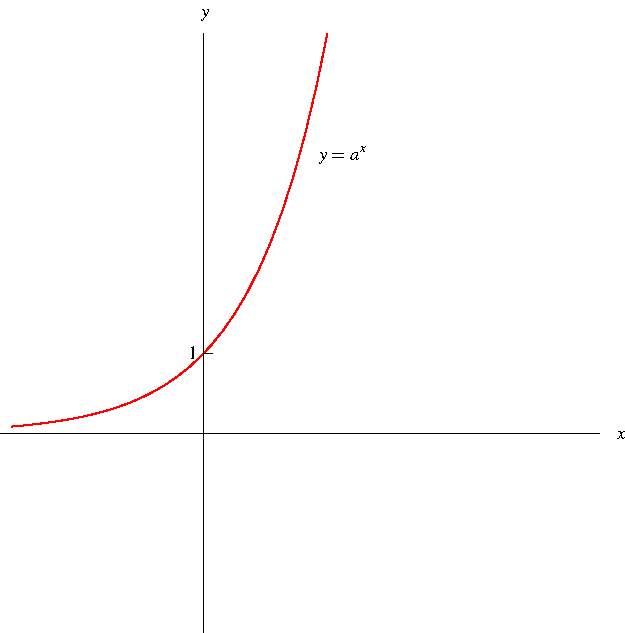
\includegraphics[height=4cm]{logarithms/pictures/07-03-logandexpa.pdf}%
%}%
%\only<8->{%
%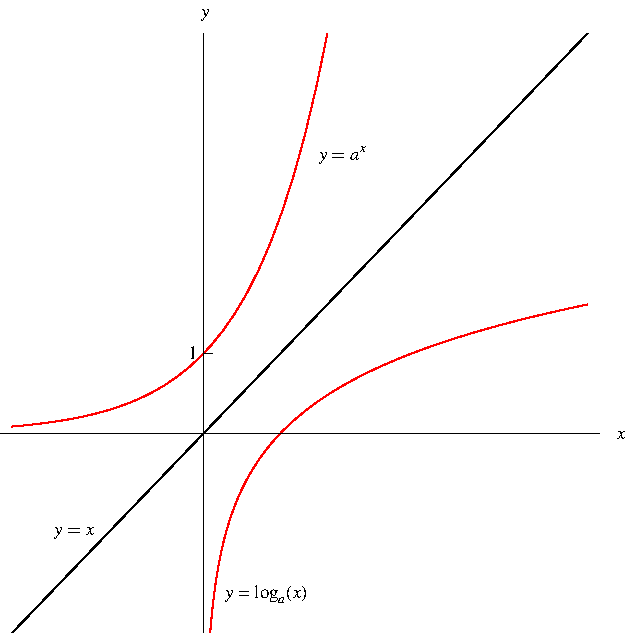
\includegraphics[height=4cm]{logarithms/pictures/07-03-logandexpb.pdf}%
%}%
\column{.7\textwidth}
\begin{itemize}
\item  Suppose $a > 0$, $a\neq 1$.
\item<2->  Let $f(x) = a^x$.
\item<3->  Then $f$ is either increasing or decreasing.
\item<4->  Therefore $f$ is one-to-one.
\item<5->  Therefore $f$ has an inverse function, $f^{-1}$.
\item<7->  The graph shows $y = a^x$ for $a > 1$.
\item<8->  The graph of $y = \log_a x$ is the reflection of this in the line $y = x$.
\end{itemize}
\end{columns}
\uncover<6->{%
\begin{definition}[$\log_a x$]
The inverse function of $f(x) = a^x$ is called the logarithmic function with base $a$, and is written $\log_a x$.  It is defined by the formula
\[
\log_a x = y \qquad \Leftrightarrow \qquad a^y = x .
\]
\end{definition}
}%
\end{frame}
% end module logarithm-def

% begin module logarithm-def-ex1
\begin{frame}
If $x > 0$, then $\log_a x$ is the exponent to which the base $a$ must be raised to give $x$.
\begin{example}%[Example 1, p. 405]
Evaluate:
\begin{enumerate}
\item<1-| alert@2-3> $\log_3 81 =$ \uncover<3->{$4$ because $3^4 = 81$.}
\item<1-| alert@4-5> $\log_{25} 5 =$ \uncover<5->{$\frac{1}{2}$ because $25^{1/2} = 5$.}
\item<1-| alert@6-7> $\log_{10} 0.001 =$ \uncover<7->{$-3$ because $10^{-3} = 0.001$.}
\end{enumerate}
\end{example}
\end{frame}
% end module logarithm-def-ex1

% begin module log-and-exp
\begin{frame}
\begin{columns}[c]
\column{.6\textwidth}
\psset{xunit=1cm, yunit=1cm}
\begin{pspicture}(-2,-2.1)(4.2, 4.2)
\psaxes[ticks=none, labels=none]{<->}(0,0)(-2,-2.1)(4.2, 4.2)
\psline(-0.1, 1)(0.1,1)
\rput[r](-0.2, 1){\footnotesize$1$}
\rput(0.9, 3){\footnotesize$y=a^x$}
%Function formula: 2^{x} 
\psplot[linecolor=red, plotpoints=1000]{-2}{2}{2 x exp }
\psplot[linecolor=red, plotpoints=1000]{0.25}{4}{x ln 0.693147181 div }
\psline[linestyle=dashed, linecolor=blue](-1.9, -1.9)(4,4) 
\rput[tl](2, 0.7){\footnotesize$y=\log_ax$}
\rput[tl](-1, -1.1){\footnotesize$y=x$}
\end{pspicture} 
%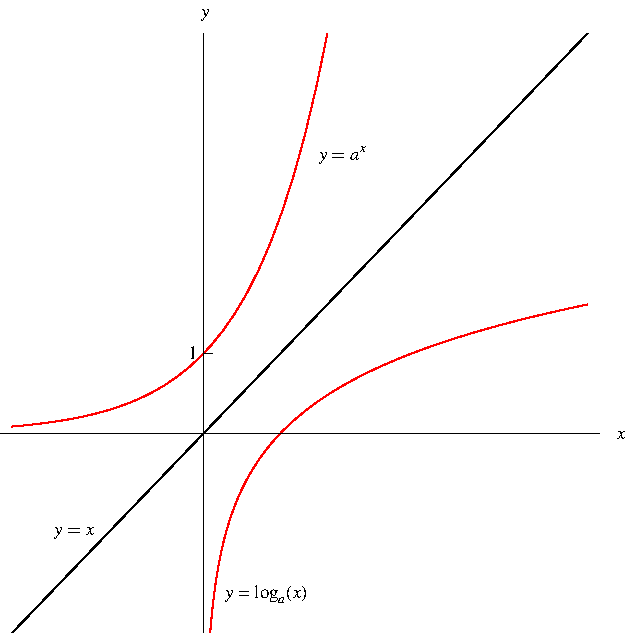
\includegraphics[height=7cm]{logarithms/pictures/07-03-logandexpb.pdf}%
\column{.4\textwidth}
\begin{itemize}
\item  Suppose $a > 1$.
\item<2-| alert@3-4>  Domain of $a^x$: \uncover<4->{$\mathbb{R}$.}
\item<2-| alert@5-6>  Range of $a^x$: \uncover<6->{$(0, \infty )$.}
\item<2-| alert@7-8>  Domain of $\log_a x$: \uncover<8->{$(0, \infty )$.}
\item<2-| alert@9-10>  Range of $\log_a x$: \uncover<10->{$\mathbb{R}$.}
\item<11->  $\log_a (a^x) = x$ for $x\in \mathbb{R}$.
\item<11->  $a^{\log_a x} = x$ for $x > 0$.
%\item<12-| alert@13-14>  $\lim_{x\rightarrow \infty}\log_a x = \uncover<14->{\infty .}$
%\item<12-| alert@15-16>  $\lim_{x\rightarrow 0^+}\log_a x = \uncover<16->{-\infty .}$
\end{itemize}
\end{columns}
\end{frame}
% end module log-and-exp

% begin module logarithm-graphs
\begin{frame}
\begin{center}
Graphs of various logarithmic functions with $a > 1$
\psset{xunit=1cm, yunit=1cm}
\begin{pspicture}(-5, -5)(5,5) 
\psframe*[linecolor=white](-5,-5)(5,5) 
\psaxes[ticks=none, labels=none]{<->}(0,0)(-0.5,-4.5)(7.5,2.5)
\psline(1,-0.1)(1,0.1)
%Function formula: ln(x)/ln(2)
\psplot[linecolor=red, plotpoints=1000]{0.044194174}{7.5}{x ln 0.693147181 div}
\rput[r](3, 1.8){\footnotesize $y=log_2 x$}
\uncover<2->{
%Function formula: ln{x}/ln(3) 
\psplot[linecolor=black, plotpoints=1000]{0.007127781}{7.5}{x ln 1.098612289 div}
\rput[l](3.6, 1.6 ){\footnotesize $y=log_3 x$}
}
\uncover<3->{
%Function formula: ln{x}/ln(5) 
\psplot[linecolor=blue, plotpoints=1000]{0.000715542}{7.5}{x ln 1.609437912 div}
\rput[l](3.7, 1.1){\footnotesize $y=log_5 x$}
}
\uncover<4->{
%Function formula: ln{x}/ln(5) 
\psplot[linecolor=green, plotpoints=1000]{0.000031623}{7.5}{x ln 2.302585093 div}
\rput[tl](3.6, 0.6){\footnotesize $y=log_{10} x$}
}
%\rput(6, 1){\color{red!1} .}
\end{pspicture} 
%\ \only<handout:0| -1>{%
%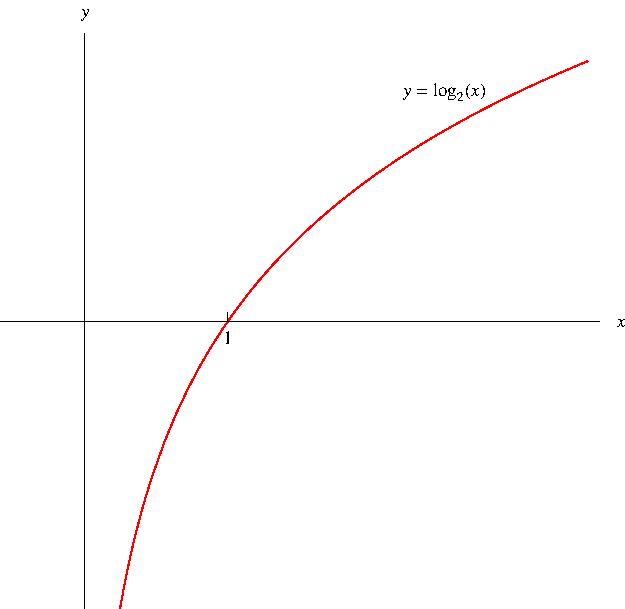
\includegraphics[height=6cm]{logarithms/pictures/07-03-manylogsa.pdf}%
%}%
%\only<handout:0| 2>{%
%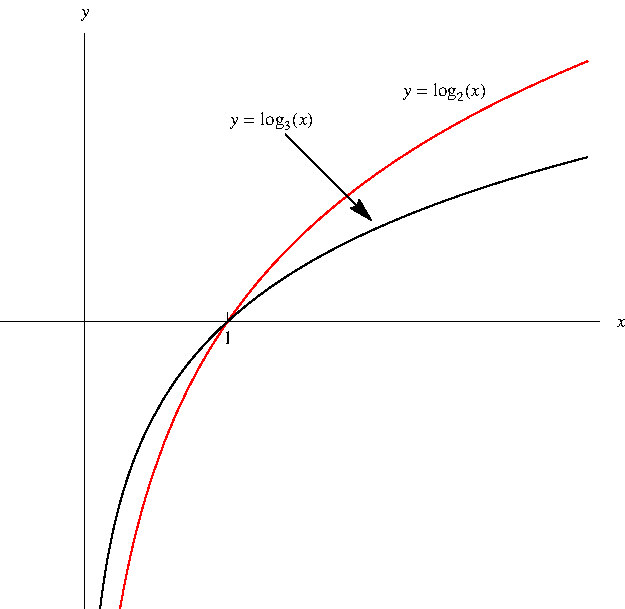
\includegraphics[height=6cm]{logarithms/pictures/07-03-manylogsb.pdf}%
%}%
%\only<handout:0| 3>{%
%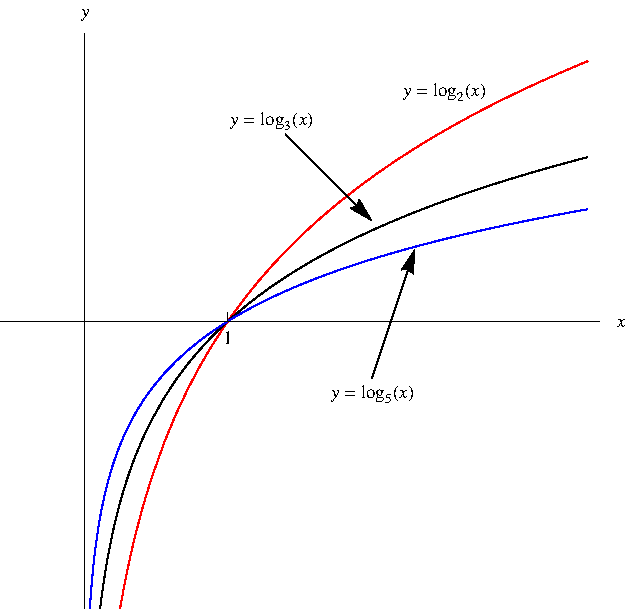
\includegraphics[height=6cm]{logarithms/pictures/07-03-manylogsc.pdf}%
%}%
%\only<4->{%
%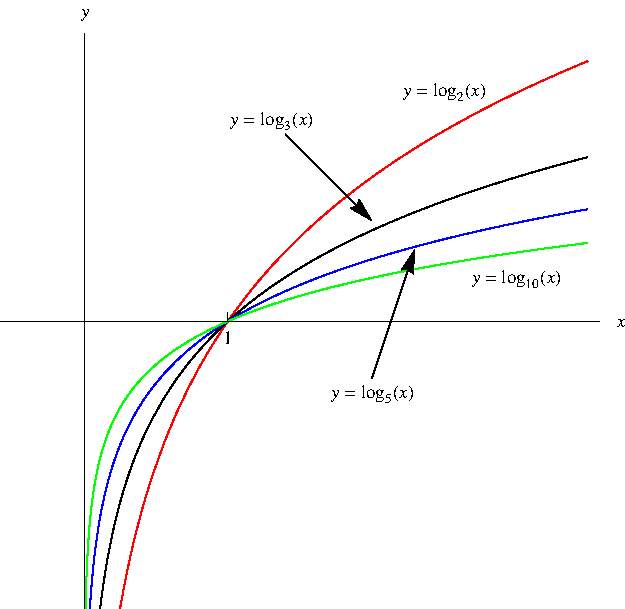
\includegraphics[height=6cm]{logarithms/pictures/07-03-manylogsd.pdf}%
%}%
\pause\pause\pause
\end{center}
\end{frame}
% end module logarithm-graphs
% begin module logarithm-properties
\begin{frame}
\begin{theorem}[Properties of Logarithmic Functions]
If $a > 1$, the function $f(x) = \log_a x$ is a one-to-one, continuous, increasing function with domain $(0, \infty )$ and range $\mathbb{R}$.  If $x, y, a, b > 0$ and $r$ is any real number, then
\begin{enumerate}
\item  $\log_a (xy) = \log_a x + \log_a y$.
\item  $\log_a \left( \frac{x}{y}\right) = \log_a x - \log_a y$.
\item  $\log_a (x^r) = r\log_a x$.
\item  $\log_{a}(x)=\log_b x \log_{a} b=\frac{\log_b x}{\log_{b} a}=  \frac{\ln x}{\ln a}$.
\end{enumerate}
\end{theorem}

\end{frame}
% end module logarithm-properties

% begin module logarithm-properties-ex2
\begin{frame}
\begin{example}
Use the properties of logarithms to evaluate the following:
\begin{columns}[t]
\column{.5\textwidth}
\begin{align*}
& \invisible{=} \log_{\alertNoH{2}{4}} \alertNoH{3}{2} + \log_{\alertNoH{2}{4}} \alertNoH{3}{32} \\
&\uncover<2->{=}  \uncover<2-| handout:0>{ \log_{ \alertNoH{2}{4}} (\alertNoH{4}{ \alertNoH{3}{2}\cdot \alertNoH{3}{32}} )} \\
&\uncover<4->{=}  \uncover<4-| handout:0>{ \alertNoH{5,6}{ \log_{ \alertNoH{7}{4}} (\alertNoH{4,9}{64})}} \\
&\uncover<5->{\alertNoH{5,6}{=}}  \fcAnswerNoH{6}{\alertNoH{8}{3}} \\
& \uncover<6-| handout:0>{\text{(because ${\alertNoH{7}{4}}^{\alertNoH{8}{3}} = \alertNoH{9}{64}$.)}}
\end{align*}
\column{.5\textwidth}
\begin{align*}
& \invisible{=} \log_{\alertNoH{10}{2}} 80 - \log_{ \alertNoH{10}{2} } 5 \\
&\uncover<10->{=}  \uncover<10-| handout:0>{ \log_{\alertNoH{10}{2}} \left(\alertNoH{11}{ \frac{80}{5}} \right) } \\
&\uncover<11->{=}  \uncover<11-| handout:0>{\alertNoH{12,13 }{ \log_{\alertNoH{14}{2}} (\alertNoH{11,16}{16})}} \\
&\uncover<12->{\alertNoH{12,13}{=}}  \fcAnswerNoH{13}{\alertNoH{15}{4}} \\
& \uncover<13-| handout:0>{\text{(because $\alertNoH{14}{2}^{\alertNoH{15}{4}} = \alertNoH{16}{16}$.)}}
\end{align*}
\end{columns}
\end{example}
\end{frame}
% end module logarithm-properties-ex2

\subsection{Natural Logarithms}
% begin module natural-logarithm-def
\begin{frame}
\frametitle{Natural Logarithms}
\begin{definition}[$\ln x$]
The logarithm with base $e$ is called the natural logarithm, and has a special notation:
\[
\log_e x = \ln x .
\]
\end{definition}
\begin{columns}[c]
\column{.5\textwidth}
\ 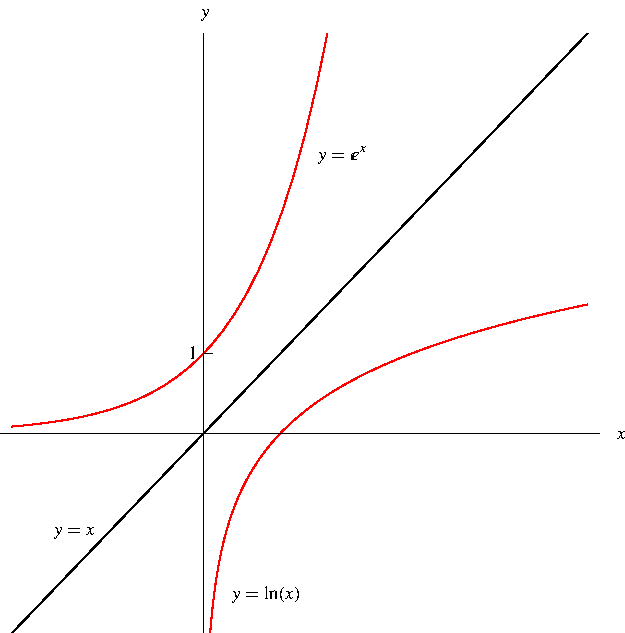
\includegraphics[height=5cm]{logarithms/pictures/07-03-natlog.pdf}%
\column{.5\textwidth}
\begin{itemize}
\item<2->  $\ln x = y \qquad \Leftrightarrow \qquad e^y = x$ .
\item<3->  $\ln (e^x ) = x$ for $x\in \mathbb{R}$.
\item<4->  $e^{\ln x}  = x$ for $x > 0$.
\end{itemize}
\end{columns}
\end{frame}
% end module natural-logarithm-def

% begin module natural-logarithm-def-ex5
\begin{frame}
\begin{example}
\begin{align*}
\text{Solve the equation} \quad e^{5-3x} & =  10 \\
\uncover<2-| handout:0>{\alertNoH{3}{\ln} ({\alertNoH{3}{e}}^{5-3x})} & \uncover<2->{=}  \uncover<2-| handout:0>{\ln 10} \\
\uncover<3-| handout:0>{\alertNoH{4}{5-}3x} & \uncover<3->{=}  \uncover<3-| handout:0>{\ln 10} \\
\uncover<4-| handout:0>{\alertNoH{5}{3}x} & \uncover<4->{=}  \uncover<4-| handout:0>{\alertNoH{4}{5-}\ln 10} \\
\uncover<5->{x} & \uncover<5->{=}  \uncover<5-| handout:0>{\frac{5-\ln 10}{\alertNoH{5}{3}}} \\
\uncover<6->{\text{Calculator:}\quad x} & \uncover<6->{\approx 0.8991.}
\end{align*}
\end{example}
\end{frame}
% end module natural-logarithm-def-ex5

% begin module exponential-equation3
\begin{frame}
\begin{columns}
\column{.55\textwidth}
\begin{example}[Finding the intersection of two exponential graphs]
Find the point(s) of intersection of $y = e^{2x}+4$ and $y = 5e^x$.  
\abovedisplayskip=0pt
\belowdisplayskip=0pt
\begin{align*}
\uncover<2->{ e^{2x} + 4 & = 5e^x }\\
\uncover<3-| handout:0>{\alert<handout:0| 5-6>{e^{2x}} - 5\alert<handout:0| 4>{e^x} + 4} & \uncover<3->{ = 0} \\
\intertext{\uncover<4->{Substitute $\alert<handout:0| 10>{u = \uncover<4-| handout:0>{e^x}}$:}}
\uncover<4-| handout:0>{\alert<handout:0| 5-6>{\uncover<6->{u^2}} - 5\alert<handout:0| 4>{u} + 4} & \uncover<4->{ = 0} \\
\uncover<7->{\alert<handout:0| 7-8>{(\uncover<8-| handout:0>{u-4})(\uncover<8-| handout:0>{u-1})}} & \uncover<7->{ = 0 } 
\end{align*}
\begin{align*}
\uncover<9->{ \alert<handout:0| 10>{u} } & \uncover<9->{=} \uncover<9-| handout:0>{ 4 } & \uncover<9->{\text{or}} & & \uncover<9->{\alert<handout:0| 10>{u}} & \uncover<9->{=} \uncover<9-| handout:0>{ 1} \\
\uncover<10-| handout:0>{ \alert<handout:0| 10>{e^x} } & \uncover<10-| handout:0>{ = 4 } & \uncover<10-| handout:0>{\text{or}} & & \uncover<10-| handout:0>{\alert<handout:0| 10>{e^x}} & \uncover<10-| handout:0>{ = 1} \invisible{99999999} \\
\uncover<11-| handout:0>{ \alert<handout:0| 11-12>{x} } & \uncover<11-| handout:0>{ \alert<handout:0| 11-12>{ = \uncover<12->{\ln 4} }} & \uncover<11-| handout:0>{\text{or}} & & \uncover<11-| handout:0>{\alert<handout:0| 13-14>{x}} & \uncover<11-| handout:0>{ \alert<handout:0| 13-14>{ = \uncover<14->{0} }} 
\end{align*}
\uncover<15-19| handout:0>{Therefore the points of intersection are \alert<handout:0| 15-16>{$(\ln 4,\uncover<16->{20})$} and \alert<handout:0| 17-18>{$(0,\uncover<18->{5})$}.}  
\end{example}

\column{.4\textwidth}

\uncover<19-| handout:0>{%
\psset{xunit=0.3cm,yunit=0.13cm,algebraic=true,dotstyle=o,dotsize=3pt 0,linewidth=0.8pt,arrowsize=3pt 2,arrowinset=0.25}
\begin{pspicture*}(-6.92,-4.61)(9.16,53.92)
\psaxes[labelFontSize=\scriptstyle,xAxis=true,yAxis=true,Dx=5,Dy=5,ticksize=-2pt 0,subticks=0]{<->}(0,0)(-6.92,-4.61)(9.16,53.92)
\psplot[linecolor=blue,plotpoints=200]{-6.915925925925918}{9.164074074074078}{5*EXP(x)}
\psplot[linecolor=red,plotpoints=200]{-6.915925925925918}{9.164074074074078}{EXP(2*x)+4}
\begin{scriptsize}
\rput[tl](2.6,40.0){$y=5e^x$}
\rput[tl](-7.0,6.5){$y=e^x+4$}
\psdots[dotstyle=*](0,5)
\rput[bl](0.1,3.99){$(0, 5)$}
\psdots[dotstyle=*](1.39,20)
\rput[bl](1.46,18.52){$(\ln4,20)$}
\end{scriptsize}
\end{pspicture*}
}%

\end{columns}
\end{frame}
% end module exponential-equation3

% begin module exponential-equation4
\begin{frame}
\begin{example}[Solving a quadratic exponential equation]
Solve for $x$.  
\abovedisplayskip=0pt
\belowdisplayskip=0pt
\begin{align*}
4^{x+1} & = 2^{x+2} + 3 \\
\uncover<2-| handout:0>{\alert<handout:0| 6>{4^{x+1}} - \alert<handout:0| 4>{2^{x+2}} - 3} & \uncover<2->{ = 0} \\
\intertext{\uncover<3->{Substitute $\alert<handout:0| 10>{u = \uncover<3-| handout:0>{2^x}}$.  Then $\alert<handout:0| 3-4>{2^{x+2} = \uncover<4-| handout:0>{4u}}$ and $\alert<handout:0| 5-6>{4^{x+1} = \uncover<6-| handout:0>{4u^2.}}$ }}
\uncover<3-| handout:0>{\alert<handout:0| 6>{\uncover<6->{4u^2}} - \alert<handout:0| 4>{\uncover<4->{4u}} - 3} & \uncover<3->{ = 0} \\
\uncover<7->{\alert<handout:0| 7-8>{(\uncover<8-| handout:0>{2u-3})(\uncover<8-| handout:0>{2u+1})}} & \uncover<7->{ = 0 } 
\end{align*}
\begin{align*}
\uncover<9->{ \alert<handout:0| 10>{u} } & \uncover<9->{=} \uncover<9-| handout:0>{ \frac{3}{2} } & \uncover<9->{\text{or}} & & \uncover<9->{\alert<handout:0| 10>{u}} & \uncover<9->{=} \uncover<9-| handout:0>{ -\frac{1}{2}} \\
\uncover<10-| handout:0>{ \alert<handout:0| 10>{2^x} } & \uncover<10-| handout:0>{ = \frac{3}{2} } & \uncover<10-| handout:0>{\text{or}} & & \uncover<10-| handout:0>{\alert<handout:0| 10>{2^x}} & \uncover<10-| handout:0>{ = -\frac{1}{2}} \invisible{99999999} \\
\uncover<11-| handout:0>{ \alert<handout:0| 11-12>{x} } & \uncover<11-| handout:0>{ \alert<handout:0| 11-12>{ = \uncover<12->{\log_2 \Big( \frac{3}{2}\Big)} }} & & & \uncover<11-| handout:0>{\alert<handout:0| 13-14>{\uncover<-13>{x}}} & \uncover<11-| handout:0>{ \alert<handout:0| 13-14>{ \only<-13>{ =} \only<14->{\text{no solution}} }} \\
\uncover<15-| handout:0>{x & = \frac{\ln (3/2)}{\ln2} & & & & } 
\end{align*}
\uncover<16-| handout:0>{Therefore the solution is $x = \frac{\ln (3/2)}{\ln 2} \approx  0.584962501$.}
\end{example}
\end{frame}
% end module exponential-equation4

% begin module natural-logarithm-def-ex8
\begin{frame}
\begin{example}%[Example 8, p. 408]
Draw the graph of $y = \ln (x - 2) -1$.
\ \only<handout:0| -1>{%
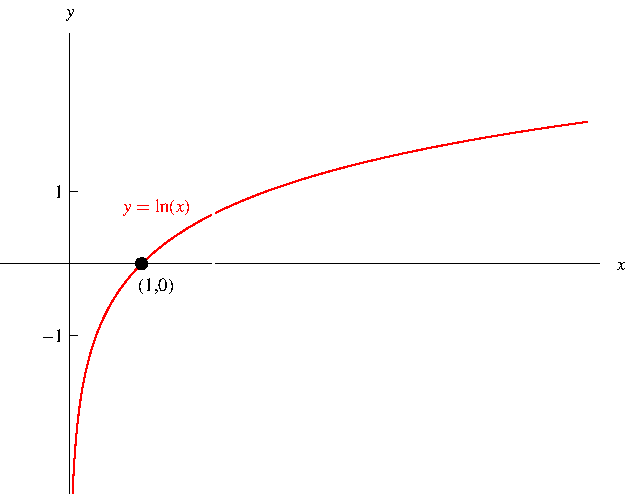
\includegraphics[height=6cm]{logarithms/pictures/07-03-ex8a.pdf}%
}%
\only<handout:0| 2>{%
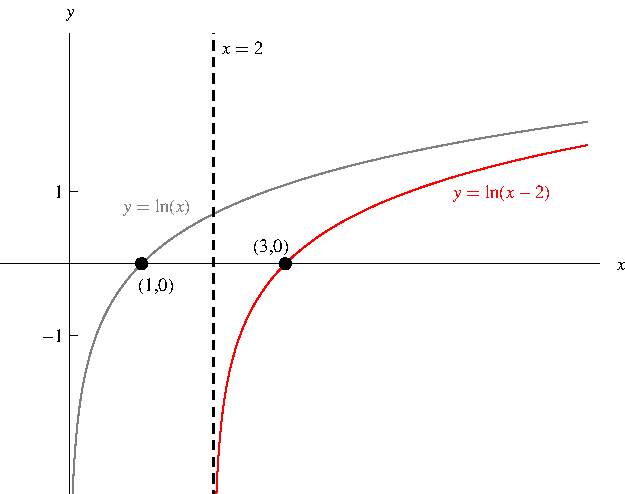
\includegraphics[height=6cm]{logarithms/pictures/07-03-ex8b.pdf}%
}%
\only<3->{%
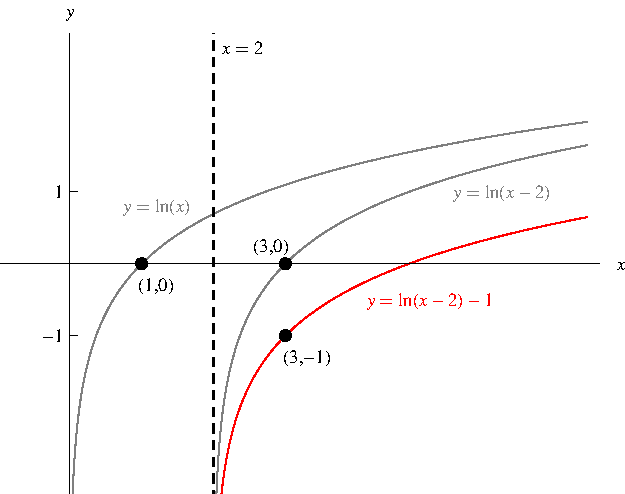
\includegraphics[height=6cm]{logarithms/pictures/07-03-ex8c.pdf}%
}%
\end{example}
\end{frame}
% end module natural-logarithm-def-ex8

%% begin module inverse-function-solve-for
\begin{frame}
%\frametitle{Inverse of a ne-to-one Function}
\begin{example}
Given: $f(x) = \frac{e^x-e^{-x}}{e^x+e^{-x}}  $.  Find $f^{-1}(x)$.
\begin{columns}
\column{0.4\textwidth}
\psset{xunit=0.8cm, yunit=0.8cm}
\begin{pspicture}(-3.05,-3.1)(3.15,3.2)
\psframe*[linecolor=white](-3.05,-3.1)(3.15,3.2)
\tiny
\psaxes[ticks=none, labels=none]{<->}(0,0)(-3.05,-3.1)(3.05,3.1)
\fcLabels{3.05}{3.1}
%Function formula: (679570457/250000000^{x}- (679570457/250000000^{- (x)}))/(679570457/250000000^{- (x)}+679570457/250000000^{x})
\uncover<1-14>{
\rput(-2,-0.5){$y=f(x)$}
\psplot[linecolor=\fcColorGraph, plotpoints=1000]{-3}{3}{2.71828 x -1 mul exp -1 mul 2.71828 x exp add 2.71828 x exp 2.71828 x -1 mul exp add div }
}
\uncover<15->{
\rput(-2,-0.5){$y=f(x)$}
\psplot[linecolor=gray!50, plotpoints=1000]{-3}{3}{2.71828 x -1 mul exp -1 mul 2.71828 x exp add 2.71828 x exp 2.71828 x -1 mul exp add div }
}
%Function formula: 1/2 (\ln{}((1+x)/(1- (x))))
\uncover<15->{
\rput[tl](1.1,2.5){$y=f^{-1}(x)$}
\psplot[linecolor=\fcColorGraph, plotpoints=1000]{-0.994}{0.994}{x 1 add x -1 mul 1 add div ln 0.5 mul }
}
\end{pspicture}
\uncover<15->{Final }\uncover<14->{answer}\uncover<15->{, \alert<15>{relabelled}:}
\[
\uncover<14->{
f^{-1}( \only<14>{y}\only<15->{\alert<15>{x}} )=\frac12\ln\frac{1+\only<14>{y}\only<15->{\alert<15>{x}} }{1-\only<14>{y}\only<15->{\alert<15>{x}}}
}
\]
\column{0.6\textwidth}
\uncover<2->{Set $u=e^x$.} \uncover<3->{Then $\alert<3>{e^{-x}=} \uncover<4->{\alert<4>{\frac1u}}$.}
\[\begin{array}{rcl}
\uncover<5->{ \frac{u-\frac1u}{u+\frac1u}&=&y}\\
\uncover<6->{\frac{u^2-1}{u^2+1}&=&y}\\
\uncover<7->{u^2-1&=&y(u^2+1)}\\
\uncover<8->{u^2(1-y)&=&1+y}\\
\uncover<9->{u^2&=&\frac{1+y}{1-y}}\\
\uncover<10->{u&=& \only<10>{\pm}\only<11>{\alert<11>{+}} \sqrt{\frac{1+y}{1-y}}}\\
\uncover<12->{\uncover<13->{x=\ln e^x =}\alert<12>{\ln} u &=& \alert<12>{\ln}\sqrt{\frac{1+y}{1-y}}}\uncover<14->{=\frac12\ln\frac{1+y}{1-y}} \\
\end{array}
\]
\uncover<11->{where the sign follows from $e^x=u>0$.} \uncover<12->{Take $\alert<12>{\ln} $ on both sides.}
\end{columns}
\end{example}
\end{frame}
% end module inverse-function-solve-for

% end lecture

% begin lecture
\lect{February 24, 2014}{Lecture  9}{9}
\section{Implicit Differentiation}
% begin module implicit-differentiation-intro
\begin{frame}
\frametitle{Implicit Differentiation}
\begin{itemize}
\item  So far, we have seen functions with formulas that express one varable explicitly in terms of the other.
\item<2->  $y = \sqrt{x^3+1}$, $y = x\sin x$, etc.
\item<3->  Some functions are given implicitly by a relation between $x$ and $y$.
\item<4->  $x^2 + y^2 = 1$ isn't the equation of any one function.
\item<5->  Implicitly it gives two functions: \uncover<6->{$\alert<6>{y = \sqrt{1-x^2}}$ and} \uncover<7->{\alert<7>{$ y = -\sqrt{1-x^2}$}.}
\item<8->  How do we differentiate these functions?
\item<9->  Differentiate both sides with respect to $x$, and then solve for $y'$.
\end{itemize}
\begin{center}
\psset{xunit=1.5cm, yunit=1.5cm}
\begin{pspicture}(-1.8, -1.15)(1.8,1.25)
\tiny
\psaxes[ticks=none, labels=none]{<->}(0,0)(-1.7,-1.15)(1.7,1.2)
\fcLabels{1.7}{1.2}
\uncover<4,5,6,8->{
\psplot[linecolor=\fcColorGraph, plotpoints=1000]{-1}{1}{x 2 exp -1 mul 1 add sqrt }
}
\uncover<7>{
\psplot[linestyle=dashed, linecolor=gray!50, plotpoints=1000]{-1}{1}{x 2 exp -1 mul 1 add sqrt }
}
\uncover<4,5,7,8->{
\psplot[linecolor=\fcColorGraph, plotpoints=1000]{-1}{1}{x 2 exp -1 mul 1 add sqrt -1 mul }
}
\uncover<6>{
\psplot[linestyle=dashed, linecolor=gray!50, plotpoints=1000]{-1}{1}{x 2 exp -1 mul 1 add sqrt -1 mul }
}
\uncover<6->{\rput[l](0.5,1){$y=\sqrt{1- x^{2}}$} }
\uncover<7->{\rput[l](0.5,-1){$y=- \sqrt{1- x^{2}}$} }
\end{pspicture}

%\ \uncover<5->{%
%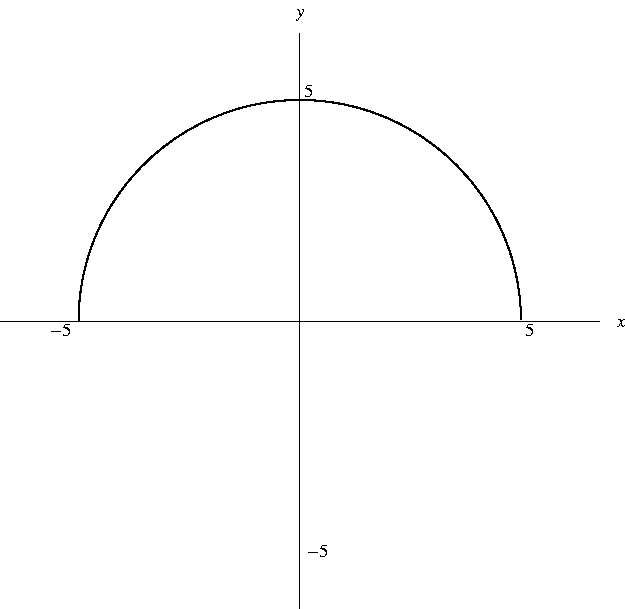
\includegraphics[height=2.5cm]{implicit-differentiation/pictures/03-06-circletop.pdf}%
%}%
%\ \uncover<4->{%
%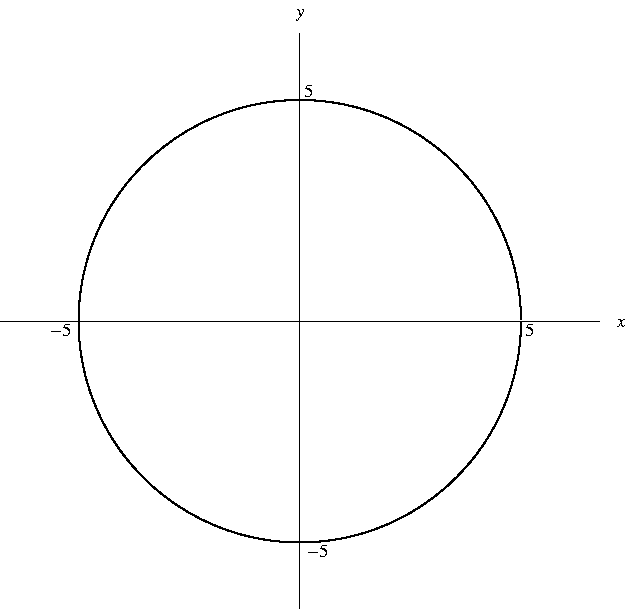
\includegraphics[height=2.5cm]{implicit-differentiation/pictures/03-06-circle.pdf}%
%}%
%\ \uncover<5->{%
%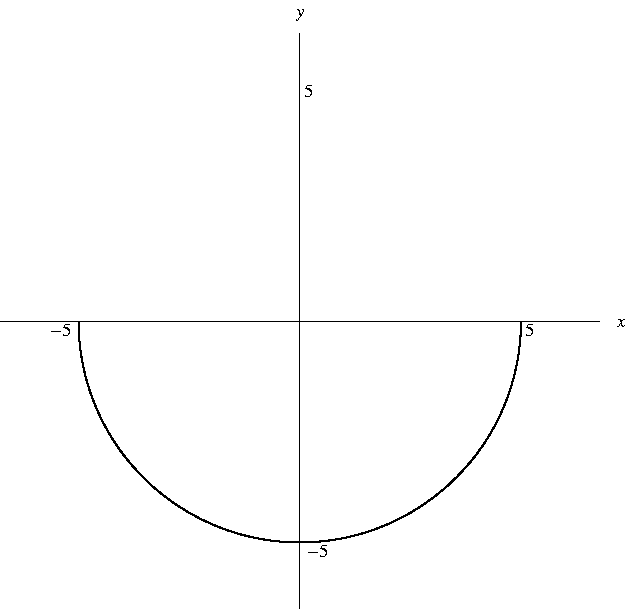
\includegraphics[height=2.5cm]{implicit-differentiation/pictures/03-06-circlebottom.pdf}%
%}%
\end{center}
\end{frame}
% end module implicit-differentiation-intro

% begin module implicit-tangent-line
\abovedisplayskip=0pt
\belowdisplayskip=0pt
\abovedisplayshortskip=0pt
\belowdisplayshortskip=0pt
\begin{frame}
\begin{example}
Find an equation of the tangent line to $(x-1)^2 + (y+2)^2 = 25$ at $(-2,2)$.
\begin{columns}
\column{1.2in}
\begin{center}
\only<handout:0|-15>{\includegraphics[height=3cm]{implicit-differentiation/pictures/implicit-tangent-line(a).jpg}}
\only<16->{\includegraphics[height=3cm]{implicit-differentiation/pictures/implicit-tangent-line(b).jpg}}
\end{center}
\begin{align*}
\uncover<15->{&\text{Plug in} \ (-2,2):}\\
\uncover<15->{&\frac{\diff y}{\diff x}  = \frac{1+2}{4} = \frac{3}{4}}\\
\uncover<16->{&\text{Point-slope form:}\\
&y-2 = \frac{3}{4} (x+2)}
\end{align*}
\column{3in}
\abovedisplayskip=0pt
\belowdisplayskip=0pt
\abovedisplayshortskip=0pt
\belowdisplayshortskip=0pt
\begin{align*}
\uncover<2->{\text{Find} \ \frac{\diff y}{\diff x}, \ \text{given} \ (x-1)^2 \ + (y+2)^2 & = 25:} \\
\uncover<3->{\alert<handout:0|3-4>{\frac{\diff}{\diff x}\left((x-1)^2\right)} + \alert<handout:0|5-6>{\frac{\diff}{\diff x}\left((y+2)^2\right)}   &= \alert<handout:0|7-8>{\frac{\diff}{\diff x}(25)}}\\
\uncover<3->{\uncover<4->{\alert<handout:0|4>{2(x-1)\alert<handout:0|9>{\frac{\diff}{\diff x}(x-1)}}} +\uncover<6->{\alert<handout:0|6>{ 2(y+2)\alert<handout:0|11-12>{\frac{\diff}{\diff x}(y+2) }}}  &= \uncover<8->{\alert<handout:0|8>{0}}}\\
\uncover<9->{2(x-1)\alert<handout:0|9-10> {(\uncover<10>{1})}+ 2(y+2)\alert<handout:0|11-12>{\left( \uncover<12->{\frac{\diff y}{\diff x}} \right)}  & = 0}\\
\uncover<13->{2(y+2)\left( \frac{\diff y}{\diff x} \right) & = -2(x-1)}\\
\uncover<14->{\frac{\diff y}{\diff x} &=  \frac{1-x}{y+2}}
\end{align*}
\end{columns}
\end{example}
\end{frame}
% end module implicit-tangent-line
% begin module implicit-differentiation-ex3
\begin{frame}
\begin{example}[Example 3, p. 213]
\abovedisplayskip=0pt
\belowdisplayskip=-15pt
\abovedisplayshortskip=0pt
\belowdisplayshortskip=0pt
\begin{align*}
\text{Find $y'$ if }\sin (x+y) & = y^2\cos x.\\
\uncover<2->{%
\alert<handout:0| 3-4>{\frac{\diff}{\diff x} (\sin (x+y))}%
}%
& \uncover<2->{ = } %
\uncover<2->{%
\alert<handout:0| 5-6>{\frac{\diff}{\diff x} (y^2\cos x)}%
}\\%
\uncover<4->{%
\alert<handout:0| 3-4>{(\cos(x+y))\alert<handout:0| 7-8>{\frac{\diff}{\diff x}(x+y)}}%
}%
& \uncover<3->{ = } %
\uncover<6->{%
\alert<handout:0| 5-6>{(y^2)\alert<handout:0| 9-10>{\frac{\diff}{\diff x}(\cos x)} + (\cos x) \alert<handout:0| 11-12>{\frac{\diff}{\diff x}(y^2)}}%
}\\%
\uncover<7->{%
(\cos(x+y))\alert<handout:0| 7-8>{\left(\uncover<8->{1+y'}\right)}%
}%
& \uncover<7->{ = } %
\uncover<7->{%
(y^2)\alert<handout:0| 9-10>{(\uncover<10->{-\sin x})} + (\cos x) \alert<handout:0| 11-12>{(\uncover<12->{2yy'})}%
}\\%
\uncover<13->{%
\cos(x+y) + y'\cos(x+y)%
}%
& \uncover<13->{ = %
-y^2\sin x +2yy'\cos x%
}\\%
\uncover<14->{%
\alert<handout:0| 15>{y'}\cos(x+y) - 2y\alert<handout:0| 15>{y'}\cos x%
}%
& \uncover<14->{ = %
-y^2\sin x -\cos(x+y)%
}\\%
\uncover<15->{%
\text{Factor:}\quad%
\alert<handout:0| 15>{y'}(\cos(x+y) - 2y\cos x)%
}%
& \uncover<15->{ = %
-y^2\sin x -\cos(x+y)%
}\\%
\uncover<16->{%
y'%
}%
& \uncover<16->{ = } %
\uncover<16->{%
\frac{-y^2\sin x - \cos(x+y)}{\cos (x+y) - 2y\cos x}.%
}%
\end{align*}
\end{example}
\end{frame}
% end module implicit-differentiation-ex3

% begin module implicit-trig
\begin{frame}
\begin{example}[Implicit Differentiation]
\abovedisplayskip=0pt
\belowdisplayskip=-15pt
\abovedisplayshortskip=0pt
\belowdisplayshortskip=0pt
\begin{align*}
\text{Find $y'$ if } \tan xy &= x^2-y^2.\\
\uncover<2->{\alert<handout:0|3-4>{\frac{\diff}{\diff x}(\tan xy)}&= \alert<handout:0|5-6>{ \frac{\diff}{\diff x}(x^2-y^2)}}\\
\uncover<3->{\alert<handout:0|4>{\uncover<4->{(\sec^2xy)\alert<handout:0|7-8>{\frac{\diff}{\diff x}(xy)}}} & = \uncover<6->{\alert<handout:0|6>{ 2x-2yy'}}}\\
\uncover<7->{\alert<handout:0|7-8>{\left(\uncover<8->{y\alert<handout:0|9-10>{\frac{\diff}{\diff x}(x)}+x\alert<handout:0|11-12>{\frac{\diff}{\diff x}(y)}}\right)}\sec^2 xy &= 2x -2yy'}\\
\uncover<9->{\left(y\alert<handout:0|9-10>{(\uncover<10->{1})}+x\alert<handout:0|11-12>{(\uncover<12->{y'})}\right)\sec^2 xy &= 2x -2yy'}\\
\uncover<13->{y\sec^2xy+xy' \sec^2xy &= 2x -2yy'}\\
\uncover<14->{xy' \sec^2xy+2yy'&=2x-y\sec^2xy}\\
\uncover<15->{y'(x\sec^2xy+2y) &= 2x-y\sec^2xy}\\
\uncover<16->{y'&=\frac{2x-y\sec^2xy}{x\sec^2xy+2y}.}
\end{align*}
\end{example}
\end{frame}
% end module implicit-trig

% begin module implicit-differentiation-ex4
\begin{frame}
\begin{example}[Example 4, p. 213]
%\uncover<2->{Differentiate implicitly:}%
\abovedisplayskip=0pt
\belowdisplayskip=0pt
\abovedisplayshortskip=0pt
\belowdisplayshortskip=0pt
\begin{align*}
\text{Find $y''$ if } \alert<handout:0| 14>{x^4 + y^4} & \alert<handout:0| 14>{ = 16}. \\
\uncover<2->{%
4x^3 + 4y^3y'%
}%
& \uncover<2->{ = } %
\uncover<2->{%
0%
}\\%
\uncover<3->{%
\alert<handout:0| 10>{y'}%
}%
& \uncover<3->{ \alert<handout:0| 10>{=} } %
\uncover<3->{%
\alert<handout:0| 10>{-\frac{x^3}{y^3}}.%
}\\%
\uncover<4->{%
y''%
}%
& \uncover<4->{ = } %
\uncover<4->{%
\frac{\diff}{\diff x}\left( -\frac{x^3}{y^3}\right)%
}  \uncover<5->{ = } %
\uncover<5->{%
- \frac{y^3 \alert<handout:0| 6-7>{\frac{\diff}{\diff x}(x^3)} - x^3\alert<handout:0| 8-9>{\frac{\diff}{\diff x}(y^3)}}{(y^3)^2}%
}\\%
& \uncover<6->{ = } %
\uncover<6->{%
- \frac{y^3 (\alert<handout:0| 6-7>{\uncover<7->{3x^2}}) - x^3(\alert<handout:0| 8-9>{\uncover<9->{3y^2\alert<handout:0| 10>{y'}}})}{y^6}%
} \uncover<10->{ = }%
\uncover<10->{%
- \frac{3x^2y^3  - 3x^3y^2\alert<handout:0| 10>{\left( -\frac{x^3}{y^3}\right)}}{y^6}%
}\\%
& \uncover<11->{ = } %
\uncover<11->{%
- \frac{3x^2(y^3+\frac{x^4}{y})}{y^6}%
} \uncover<12->{ = }%
\uncover<12->{%
- \frac{3x^2\left( \frac{y^4+x^4}{\alert<handout:0| 13>{y}}\right)}{\alert<handout:0| 13>{y^6}}%
}\\%
& \uncover<13->{ = } %
\uncover<13->{%
- \frac{3x^2(\alert<handout:0| 14>{y^4+x^4})}{\alert<handout:0| 13>{y^7}}%
}  \uncover<14->{ = }%
\uncover<14->{%
- \frac{3x^2(\alert<handout:0| 14>{16})}{y^7}%
} \uncover<15->{ = }%
\uncover<15->{%
-48 \frac{x^2}{y^7}.%
}%
\end{align*}
\end{example}
\end{frame}
% end module implicit-differentiation-ex4

%\input{../../modules/implicit-differentiation/implicit-second-derivative}
% begin module exponential-equation4
\begin{frame}
\begin{example}[Solving a quadratic exponential equation]
Solve for $x$.  
\abovedisplayskip=0pt
\belowdisplayskip=0pt
\begin{align*}
4^{x+1} & = 2^{x+2} + 3 \\
\uncover<2-| handout:0>{\alert<handout:0| 6>{4^{x+1}} - \alert<handout:0| 4>{2^{x+2}} - 3} & \uncover<2->{ = 0} \\
\intertext{\uncover<3->{Substitute $\alert<handout:0| 10>{u = \uncover<3-| handout:0>{2^x}}$.  Then $\alert<handout:0| 3-4>{2^{x+2} = \uncover<4-| handout:0>{4u}}$ and $\alert<handout:0| 5-6>{4^{x+1} = \uncover<6-| handout:0>{4u^2.}}$ }}
\uncover<3-| handout:0>{\alert<handout:0| 6>{\uncover<6->{4u^2}} - \alert<handout:0| 4>{\uncover<4->{4u}} - 3} & \uncover<3->{ = 0} \\
\uncover<7->{\alert<handout:0| 7-8>{(\uncover<8-| handout:0>{2u-3})(\uncover<8-| handout:0>{2u+1})}} & \uncover<7->{ = 0 } 
\end{align*}
\begin{align*}
\uncover<9->{ \alert<handout:0| 10>{u} } & \uncover<9->{=} \uncover<9-| handout:0>{ \frac{3}{2} } & \uncover<9->{\text{or}} & & \uncover<9->{\alert<handout:0| 10>{u}} & \uncover<9->{=} \uncover<9-| handout:0>{ -\frac{1}{2}} \\
\uncover<10-| handout:0>{ \alert<handout:0| 10>{2^x} } & \uncover<10-| handout:0>{ = \frac{3}{2} } & \uncover<10-| handout:0>{\text{or}} & & \uncover<10-| handout:0>{\alert<handout:0| 10>{2^x}} & \uncover<10-| handout:0>{ = -\frac{1}{2}} \invisible{99999999} \\
\uncover<11-| handout:0>{ \alert<handout:0| 11-12>{x} } & \uncover<11-| handout:0>{ \alert<handout:0| 11-12>{ = \uncover<12->{\log_2 \Big( \frac{3}{2}\Big)} }} & & & \uncover<11-| handout:0>{\alert<handout:0| 13-14>{\uncover<-13>{x}}} & \uncover<11-| handout:0>{ \alert<handout:0| 13-14>{ \only<-13>{ =} \only<14->{\text{no solution}} }} \\
\uncover<15-| handout:0>{x & = \frac{\ln (3/2)}{\ln2} & & & & } 
\end{align*}
\uncover<16-| handout:0>{Therefore the solution is $x = \frac{\ln (3/2)}{\ln 2} \approx  0.584962501$.}
\end{example}
\end{frame}
% end module exponential-equation4

% end lecture

% begin lecture
\lect{March 7, 2014}{Lecture 12}{12}
\section{Derivatives of Logarithmic and Exponential Functions}
\subsection{Derivatives of General Exponential Functions}
% begin module chain-rule-general-exponential.tex
\begin{frame}
\begin{example}[Chain Rule, general exponential function]
\begin{align*}
\text{Differentiate}\quad y & = \alert<handout:0|2-3>{2}^x.\\
\uncover<2->{y} & \uncover<2->{= \alert<handout:0|2-3>{( e^{\uncover<3->{\ln 2}} )}^x}\\
\uncover<4->{y} & \uncover<4->{= e^{x\ln 2}.}\\
\uncover<5->{\text{Let} \quad \alert<handout:0|5-6>{\alert<handout:0|13-14>{\alert<handout:0|11-12>{u}}} &\alert<handout:0|5-6>{\alert<handout:0|11-14>{=}} \uncover<6->{\alert<handout:0|6>{\alert<handout:0|11-12>{\alert<handout:0|13-14>{ x\ln 2.}}}}} \\
\uncover<7->{\text{Then} \quad \alert<handout:0|9-10>{y} &\alert<handout:0|9-10>{= e^u.}} \\
\uncover<8->{\text{Chain Rule:}\quad \frac{\diff y}{\diff x} &= \alert<handout:0|9-10>{ \frac{\diff y}{\diff u}}\alert<handout:0|11-12>{ \frac{\diff u}{\diff x}}}\\
\uncover<9->{&= \alert<handout:0|9-10>{(\uncover<10->{e^{\alert<handout:0|13-14>{u}}})}\alert<handout:0|11-12>{(\uncover<12->{\ln 2})} }\\
\uncover<13->{ &= (e^{\alert<handout:0|13-14>{(\uncover<14->{x\ln2})}})(\ln 2)}\\
\uncover<15->{& = (2^x)(\ln 2)} 
\end{align*}
\end{example}
\end{frame}
% begin module chain-rule-general-exponential.tex
% begin module general-exponential-derivative
\begin{frame}
\begin{theorem}[The Derivative of $a^x$]
\[
\frac{\diff}{\diff x} (a^x) = a^x \ln a .
\]
\end{theorem}
\end{frame}
% end module general-exponential-derivative

% begin module chain-rule-twice-ex1
\begin{frame}
\chainruletwice%
{\sin\sqrt{10^x+1}}%
{\cos\sqrt{10^x+1}}%
{\sqrt{10^x+1}}%
{\frac{1}{2\sqrt{10^x+1}}}%
{10^x+1}%
{10^x\ln 10}%
{}%
{\frac{(\ln 10)10^x\cos \sqrt{10^x+1}}{2\sqrt{10^x+1}}}%
{}%
\end{frame}
% end module chain-rule-twice-ex1

\subsection{Derivatives of Logarithmic Functions}
% begin module general-log-derivative-implicit
\begin{frame}
\frametitle{Derivatives of Logarithmic Functions}
\begin{theorem}[The Derivative of $\log_a x$]
\[
\frac{\diff}{\diff x} (\log_a x) = \frac{1}{x\ln a} .
\]
\end{theorem}
\begin{proof}
\abovedisplayskip=0pt
\belowdisplayskip=0pt
\abovedisplayshortskip=0pt
\belowdisplayshortskip=0pt
\begin{align*}
\uncover<2->{%
\text{Let } y %
}%
& \uncover<2->{%
 = \log_a x. %
}\\%
\uncover<3->{%
\text{Then } \alertNoH{ 4-5,9}{a^y} %
}%
& \uncover<3->{%
 \alertNoH{ 9}{=} \alertNoH{ 6-7,9}{x}. %
}\\%
\uncover<4->{%
\text{Differentiate implicitly:}\quad \alertNoH{ 4-5}{\fcAnswer{5}{a^y (\ln a) y'}} %
}%
& \uncover<4->{%
 = \alertNoH{ 6-7}{\fcAnswerUncover{4}{7}{1}} %
}\\%
\uncover<8->{%
y' %
}%
& \uncover<8->{%
 = \frac{1}{\alertNoH{ 9}{a^y}\ln a} %
}\\%
& \uncover<9->{%
 = \frac{1}{\alertNoH{ 9}{x}\ln a}. %
}%
\end{align*}
\end{proof}
\end{frame}
% end module general-log-derivative-implicit

% begin module general-log-derivative-ex.tex
\begin{frame}
\chainrulefofx{\log_3(5^{x}+1)}{5^x+1}{\log_3 x}{\frac{1}{ UU \ln 3}}{5^x \ln 5 }{\frac{5^x \ln 5}{(5^x+1) \ln 3}}{0}
\end{frame}
% end module general-log-derivative-ex.tex
% begin module natural-log-derivative-from-general
\begin{frame}
\begin{theorem}[The Derivative of $\log_a x$]
\[
\frac{\diff}{\diff x} (\log_a x) = \frac{1}{x\ln a} .
\]
\end{theorem}

$\ln x = \log_e x$. Therefore when we set $a = e$ we get the derivative of $\ln x$:
\begin{align*}
\frac{\diff}{\diff x}(\ln x) & = \frac{1}{x\alertNoH{ 2-3}{\ln e}} \\
 & \uncover<2->{= \frac{1}{x\alertNoH{2-3}{( \fcAnswer{3}{1}) }}} \\
 & \uncover<4->{= \frac{1}{x}.}
\end{align*}
\uncover<5->{%
\begin{theorem}[The Derivative of $\ln x$]
\[
\frac{\diff}{\diff x} (\ln x) = \frac{1}{x}.
\]
\end{theorem}
}%
\end{frame}
% end module natural-log-derivative-from-general

% begin module natural-log-derivative-ex-simplify.tex
\begin{frame}
\begin{example}[Chain Rule, Natural Logarithm]
\abovedisplayskip=0pt
\belowdisplayskip=0pt
\abovedisplayshortskip=0pt
\belowdisplayshortskip=0pt
\begin{align*}
\text{Differentiate}\quad y &= \ln (e^x \sec x).\\
\uncover<2->{ y&= \alert<handout:0|3-4>{\ln e^x} + \ln \sec x}\\
\uncover<3->{ &=\uncover<4->{\alert<handout:0|4>{\alert<handout:0|5-6>{ x}}} + \ln \sec x.}\\
\uncover<5->{\frac{\diff y}{\diff x} & =\uncover<6->{\alert<handout:0|6>{1} }+ \uncover<7->{ \alert<handout:0|7>{\alert<handout:0|11>{\frac{\diff}{\diff x} (\ln \sec x)}}}}\\
\uncover<8->{\alert<handout:0|8-9>{\text{Let} \ \ \alert<handout:0|14-16>{u} }&  \alert<handout:0|8-9>{\alert<handout:0|14-16>{= \uncover<9->{ \sec x.}}}}\\
\uncover<10->{\text{Then} \ \ \ln \sec x & = { \ln u}.}\\
\uncover<11->{\text{Chain Rule:} \quad \frac{\diff y}{\diff x} & = 1+  \alert<handout:0|11>{\alert<handout:0|12-13>{\frac{\diff}{\diff u}(\ln u)} \alert<handout:0|14-15>{\frac{\diff u}{\diff x}}}}\\
\uncover<12->{& = 1+ \alert<handout:0|12-13>{\left( \uncover<13->{\frac{1}{\alert<handout:0|16>{u}}} \right)} \alert<handout:0|14-15>{(\uncover<15->{\sec x \tan x} )} }\\
\uncover<16->{& = 1+ \frac{1}{\alert<handout:0|16>{\sec x}}\sec x \tan x} \\
\uncover<17->{& = 1+ \tan x.}
\end{align*}
\end{example}
\end{frame}
% begin module natural-log-derivative-ex-simplify.tex
% begin module natural-logarithm-derivative-ex7
\begin{frame}
\begin{example}
\abovedisplayskip=0pt
\belowdisplayskip=0pt
\abovedisplayshortskip=0pt
\belowdisplayshortskip=0pt
\begin{align*}
\text{Find $f'(x)$ if } f(x) & = \ln |x|.\\
\uncover<2->{%
f(x) %
}% 
& \uncover<2->{
 = \left\{ \begin{array}{lr}
\alert<handout:0| 3-4>{\ln x} & \text{ if } x > 0 \\
\alert<handout:0| 5-6>{\ln (-x)} & \text{ if } x < 0 \\
\end{array}\right. .
}\\%
\uncover<3->{%
f'(x) %
}%
& \uncover<3->{
 = \left\{ \begin{array}{lr}
\alert<handout:0| 3-4>{\uncover<4->{\frac{1}{x}}} & \text{ if } x > 0 \\
\alert<handout:0| 5-6>{\uncover<6->{\frac{1}{-x}(-1)}} & \text{ if } x < 0 \\
\end{array}\right.
}\\%
& \uncover<7->{
 = \left\{ \begin{array}{lr}
\frac{1}{x} & \text{ if } x > 0 \\
\frac{1}{x} & \text{ if } x < 0 \\
\end{array}\right.
}\\%
& \uncover<8->{%
 = \frac{1}{x} \text{ if } x \neq 0.
}%
\end{align*}
\end{example}
\end{frame}
% end module natural-logarithm-derivative-ex7

\subsection{Logarithmic Differentiation}
% begin module logarithmic-differentiation-ex.tex
\begin{frame}
\begin{example}[Logarithmic Differentiation]
\abovedisplayskip=0pt
\belowdisplayskip=0pt
\abovedisplayshortskip=0pt
\belowdisplayshortskip=0pt

\begin{align*}
\text{Differentiate} \quad \alert<handout:0|13>{y} &\alert<handout:0|13>{= \frac{(x-1)^{5/3} \sin^3 x}{\sqrt{e^x + 1}}}.\\
\intertext{\uncover<2->{Take the natural logarithm of both sides:}}
\uncover<2->{\ln y &= \ln  \frac{(x-1)^{5/3} \sin^3 x}{\sqrt{e^x + 1}} }\\
\uncover<3->{ \ln y &=(5/3) \ln(x-1) +3\ln \left( \sin x\right)-(1/2)\ln\left(e^x + 1\right).}\\
\uncover<4->{\alert<handout:0|4-5>{\frac {\diff }{\diff x} (\ln y)} &= \alert<handout:0|6-11>{ \frac{\diff}{\diff x}} \left[ \alert<handout:0|6-7>{ (5/3) \ln(x-1)} +\alert<handout:0|8-9>{3\ln \left( \sin x\right)}-\alert<handout:0|10-11>{(1/2)\ln\left(e^x + 1\right)}\right]}\\
\uncover<4->{ \alert<handout:0|4-5>{\left[ \uncover<5->{\frac{1}{y} \left(\frac {\diff y}{\diff x}\right)}\right]} &= \alert<handout:0|6-7>{ \left[\uncover<7->{ \frac{5}{3}\left(\frac{1}{x-1} \right)}  \right] }+ \alert<handout:0|8-9>{ \left[ \uncover<9->{ \frac{3\cos x}{\sin x}} \right] }- \alert<handout:0|10-11>{\left[\uncover<11->{ \frac{1}{2} \left(\frac{e^x}{e^x+1}  \right)} \right]}}\\
 \uncover<12->{\frac {\diff y}{\diff x} &=  \left( \frac{5}{3(x-1)}  + 3\cot x -\frac{e^x}{2(e^x+1)} \right)\alert<handout:0|13>{y}}\\
 \uncover<13->{& = \left( \frac{5}{3(x-1)}  + 3\cot x -\frac{e^x}{2(e^x+1)} \right) \alert<handout:0|13>{\frac{(x-1)^{5/3} \sin^3 x}{\sqrt{e^x + 1}}}.}
\end{align*}

\end{example}
\end{frame}
% begin module logarithmic-differentiation-ex.tex
% begin module logarithmic-differentiation
\begin{frame}
Steps in Logarithmic Differentiation
\begin{enumerate}
\item  Take natural logarithms of both sides of an equation $y = f(x)$ and use the properties of logarithms to simplify.
\item  Differentiate implicitly with respect to $x$.
\item  Solve the resulting equation for $y'$.
\end{enumerate}
Note: If $f(x) < 0$, then $\ln (f(x))$ is not defined, but we can write $|y| = |f(x)|$ and use the result of example 6, p. 223.
\end{frame}
% end module logarithmic-differentiation

% begin module logarithmic-differentiation-ex-base-and-power2
\begin{frame}
\logdiffbaseandexp{x}{\tan x}{\frac{1}{x}}{\sec^2 x}{\frac{\tan x}{x} + (\ln x)\sec^2 x}
\end{frame}
% end module logarithmic-differentiation-ex-base-and-power2

% end lecture

% begin lecture
\lect{March 10, 2014}{Lecture 13}{13}
\section{Inverse Trigonometric Functions}
% begin module arcsin-def
\begin{frame}
\frametitle{Inverse Trigonometric Functions}
\psset{xunit=0.6cm,yunit=0.6cm}
\begin{pspicture}(-5,-1.9)(10,1.9)
\tiny
\psaxes[labels=none, Dx=1.570796327, Dy=1] {<->}(0,0)(-4,-1.8)(10,1.8)

\uncover<1-2| handout:0>{\psplot[linecolor=red, plotpoints=1000]{-4}{10}{x 57.295779513 mul sin}}
\uncover<2| handout:0>{\psline(-4,0.6)(10,0.6 )}

\uncover<3>{\psplot[linecolor=red, plotpoints=1000]{-1.570796327}{1.570796327}{x 57.295779513 mul sin}
\rput[bl](3, 1){\alertNoH{3}{$y=\sin x, -\frac{\pi}{2}\leq x\leq \frac{\pi}{2}$} }
}
\uncover<4-| handout:1>{\psplot[linecolor=gray, plotpoints=1000]{-1.570796327}{1.570796327}{x 57.295779513 mul sin}
\rput[bl](3, 1){\color{gray}{$y=\sin x, -\frac{\pi}{2}\leq x\leq \frac{\pi}{2}$} }
}
\uncover<4|handout:1>{\psline[linecolor=blue, linestyle=dashed](-1.75,-1.75)(1.75,1.75)}
\uncover<4-| handout:1>{\psplot[linecolor=red, plotpoints=1000]{-1}{1}{x ASIN}
\rput[r](-1.5, -1){\alertNoH{4}{$y=\Arcsin x$} }}

\rput[t](-3.14, -0.3){$-\pi$}
\rput[t](-1.57, -0.3){$-\frac{\pi}{2}$}
\rput[t](1.57, -0.3){$\frac{\pi}{2}$}
\rput[t](3.14, -0.3){$\pi$}
\rput[t](4.71, -0.3){$\frac{3\pi}{2}$}
\rput[t](6.28, -0.3){$2\pi$}
\rput[t](7.85, -0.3){$\frac{5\pi}{2}$}
\rput[t](9.42, -0.3){$3\pi$}
\rput[bl](0.2,1){\tiny $1$}
\end{pspicture}
\begin{columns}[c]
\column{.65\textwidth}
\begin{itemize}
\item<2->  $\sin x$ isn't one-to-one.
\item<3->  It is if we restrict the domain to $\left[-\frac{\pi}{2}, \frac{\pi}{2}\right]$.
\item<4->  Then it has an inverse function.
\item<4->  We call it $\arcsin$ or $\sin^{-1}$.
\item<6->  $\Arcsin x = y \Leftrightarrow \sin y = x$ and $-\frac{\pi} {2} \leq y \leq \frac{\pi}{2}$.
\end{itemize}
\column{.35\textwidth}
\psset{xunit=1cm,yunit=1cm}
\uncover<5->{
\begin{pspicture}(-1.5,-2)(1.7,2)
\tiny
\psaxes[ticks=none, labels=none]{<->}(0,0)(-1.5,-2)(1.5,2)
\fcLabels{1.5}{2}
\fcLabelXOne
\psline(-1, -0.1)(-1,0.1)
\rput[t](-1,  -0.1){$-1$}

\psline(-0.1, 1.570796327)(0.1,1.570796327)
\rput[r](-0.1,  1.570796327){$\frac{\pi}{2}$}
\psline(-0.1, -1.570796327)(0.1,-1.570796327)
\rput[r](-0.1,  -1.570796327){$-\frac{\pi}{2}$}

\psplot[linecolor=red, plotpoints=1000]{-1}{1}{x ASIN}
\rput[rb](-0.05, 0.2){\alertNoH{4}{$y=\Arcsin x$} }
\fcFullDot{1}{1.570796327}
\fcFullDot{-1}{-1.570796327}
\end{pspicture}
}
%\uncover<5->{%
%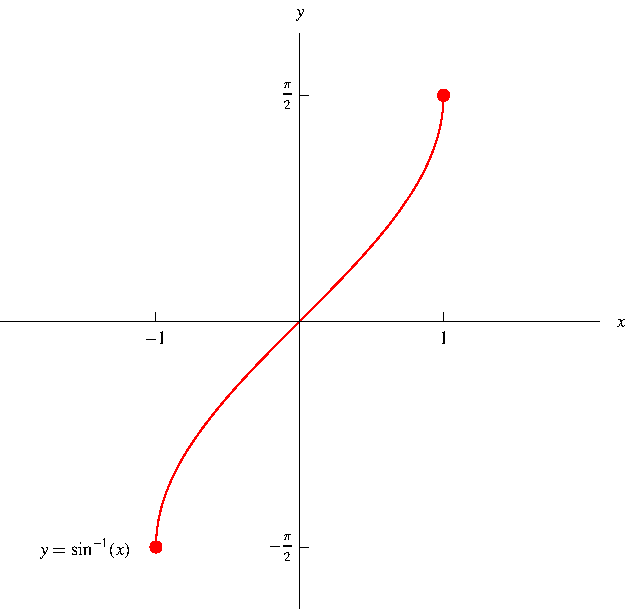
\includegraphics[height=4cm]{inverse-trig/pictures/07-06-arcsine.pdf}%
%}%

\end{columns}
\end{frame}
% end module arcsin-def

% begin module arcsin-sin-ex1
\begin{frame}
\begin{example}
Find $\Arcsin (\sin 1.5)$.  
\begin{itemize}
\item<2->  \alert<2-3>{$\pi/2 \approx \uncover<3->{1.57.}$}
\item<4->  Therefore $-\pi/2 \leq 1.5\leq \pi/2$.  
\item<5->  Therefore $\Arcsin (\sin 1.5) = 1.5$.  
\end{itemize}
\end{example}
\end{frame}
% end module arcsin-sin-ex1

% begin module arcsin-sin-ex2
\begin{frame}
\begin{example}
Find $\Arcsin (\sin 2)$.
\begin{itemize}
\item<2-> $2$ is not between $-\frac{\pi}{2}$ and $\frac{\pi}{2}$.
\item<3-> We need the angle \alertNoH{8,12}{$a$ between $-\frac{\pi}{2}$ and $\frac{\pi}{2}$} for which $\alertNoH{11}{ \alertNoH{4}{ \sin 2} =\alertNoH{7}{ \sin a}}$.
\end{itemize}
\uncover<9->{
\[
\begin{array}{rcl}
\alertNoH{9,10,13}{a} &\alertNoH{9,10,13}{=}& \fcAnswer{10}{ \alertNoH{13}{\pi - 2}.} \\
\uncover<11->{\text{Therefore }\quad \Arcsin(\alertNoH{11}{\sin 2}) &\alertNoH{0}{ =} & \alertNoH{12}{\Arcsin(\alertNoH{11}{\sin a})}} \\
\uncover<12->{&\alertNoH{0}{ =}& \worksheet{ \alertNoH{12,13}{ a} \uncover<13->{\alertNoH{13}{= \pi-2}.}}}
\end{array}
\]
}
\end{example}

\hfill
\psset{xunit=1.5cm, yunit=1.5cm}
\begin{pspicture}(-1.4,-1.4)(1.4,1.4)
\tiny
\fcAxesStandard{-1.2}{-1.2}{1.2}{1.2}
\parametricplot[linecolor=gray]{0}{360}{t cos t sin}%
\parametricplot[linecolor=brown]{-90}{90}{t cos t sin}%
\fcXTickWithLabel{1}{$1$}
\pstVerb{20 dict begin /pi 3.141592654 def /toDeg {180 mul pi div} def}%
\uncover<2->{%
\psline[arrows=->](0,0)(! 2 toDeg cos 1.3 mul 2 toDeg sin 1.3 mul)%
\parametricplot[linecolor=orange]{0}{2 toDeg}{t cos 0.35 mul t sin 0.35 mul}%
\rput[bl](0.24, 0.27){$2 $}
}%
\worksheet{%
\uncover<4->{\fcPerpendicular[linecolor=blue]{[2 toDeg cos 2 toDeg sin]}{[1 0]}{0.1}}%
\uncover<handout:0|4>{\psline[linecolor=blue, linewidth=2pt](! 2 toDeg cos 2 toDeg sin)(! 2 toDeg cos 0)}%
\uncover<5->{\parametricplot[linecolor=green]{2 toDeg}{180}{t cos 0.15 mul t sin 0.15 mul}%
\rput[br](-0.15, 0.15){$\fcAnswer{10}{\pi-2}$}%
}%
\uncover<handout:0|10>{%
\parametricplot[linewidth=2pt, linecolor=green]{2 toDeg}{180}{t cos 0.15 mul t sin 0.15 mul}%
\parametricplot[linewidth=2pt, linecolor=green]{0}{pi 2 sub toDeg}{t cos 0.15 mul t sin 0.15 mul}%
}%
\uncover<6->{%
\psline[linestyle=dotted](! 2 toDeg cos 2 toDeg sin)(! pi 2 sub toDeg cos pi 2 sub toDeg sin)%
}%
\uncover<7->{%
\fcPerpendicular[linecolor=blue]{[pi 2 sub toDeg cos pi 2 sub toDeg sin]}{[-1 0]}{0.1}%
\psline[arrows=->](0,0)(! pi 2 sub toDeg cos 1.3 mul pi 2 sub toDeg sin 1.3 mul)%
}%
\uncover<handout:0|7>{\psline[linecolor=blue, linewidth=2pt](! pi 2 sub toDeg cos pi 2 sub toDeg sin)(! pi 2 sub toDeg cos 0)}%
\uncover<8->{%
\parametricplot[linecolor=green]{0}{pi 2 sub toDeg}{t cos 0.15 mul t sin 0.15 mul}%
\rput[lb](0.15, 0.07){$\alertNoH{9,10}{a}$}%
}%
}%
\pstVerb{end}
\end{pspicture} \quad 
\psset{xunit=1.0cm,yunit=1.0cm}
\begin{pspicture}(-2.2,-1.9)(4.2,1.9)
\tiny
\pstVerb{20 dict begin /pi 3.141592654 def /toDeg {180 mul pi div} def}%
\psaxes[labels=none, Dx=1.570796327, Dy=1] {<->}(0,0)(-2,-1.8)(4,1.8)
\psline[linecolor=brown, linewidth=1.05pt](! pi -2 div 0)(! pi 2 div 0)
\psplot[linecolor=blue, plotpoints=1000]{-1.570796327}{1.570796327}{x 57.295779513 mul sin}
\rput[bl](3, 1){$y=\sin x$ }
\psplot[linecolor=gray, plotpoints=1000]{pi 2 div}{4}{x 57.295779513 mul sin}
\psplot[linecolor=gray, plotpoints=1000]{-2}{pi -2 div}{x 57.295779513 mul sin}
\rput[t](-1.57, -0.3){$-\frac{\pi}{2}$}
\rput[t](1.57, -0.3){$\frac{\pi}{2}$}
\rput[t](3.14, -0.3){$\pi$}
\rput[bl](0.2,1){\tiny $1$}
\worksheet{%
\uncover<4->{\psline[linecolor=blue](2,0)(! 2 2 toDeg sin)}%
\uncover<7->{\psline[linecolor=blue](! pi 2 sub 0)(! pi 2 sub dup toDeg sin)}%
}
\uncover<2->{\fcXTickWithLabel{2}{$2$}}%
\worksheet{%
\uncover<7->{\fcXTickWithLabel{pi 2 sub}{$\uncover<8->{a}$}}%
\uncover<6->{\psline[linestyle=dotted](! pi 2 sub 0.909297427)(2,0.909297427)}%
\uncover<5->{\psline[linecolor=green]{<->}(2,-0.2)(! pi -0.2)}%
\uncover<8->{\psline[linecolor=green]{<->}(0,-0.2)(! pi 2 sub -0.2)}%
}%
\pstVerb{end}
\end{pspicture}
\hfill
\end{frame}
% end module arcsin-sin-ex2

% begin module arcsin-ex1
\begin{frame}
\vskip -0.1cm
\begin{example}
\begin{columns}[t]
\column{.3\textwidth}
\hfil \hfil Find $\displaystyle \Arcsin \left( \frac{1}{2}\right)$.
\begin{itemize}
\item<2->  $\displaystyle \sin \left(\uncover<2-| handout:0>{\frac{\pi}{ 6}}\right) = \frac{1}{2}$.
\item<3->  $\displaystyle -\frac{\pi}{2} \leq \uncover<3-| handout:0>{\frac{\pi}{6}} \leq \frac{\pi}{2}$.
\item<4->  Therefore $ \Arcsin \left( \frac{1}{2}\right) = \uncover<3-| handout:0>{\frac{\pi}{6}}$.
\end{itemize}
\column{.7\textwidth}
\hfil \hfil Find $\displaystyle
\tan \left( \Arcsin \left( \frac{1}{3}\right) \right)
$.
\begin{itemize}
\item<5->  Let $\theta = \Arcsin \left(\frac{1}{3}\right)$, so $\sin \theta = \frac{ \alertNoH{6}{1}}{\alertNoH{7}{3}}$.
\item<6->  Draw a right triangle with  \alertNoH{6}{opposite side $1$} and \alertNoH{7}{hypotenuse $3$}.
\item<8-> Let the angle $\theta$ be as labeled. \uncover<9->{ Then $ \alertNoH{9,10}{\sin\theta= \frac{1 }{3}}$ \uncover<10->{and so $\alertNoH{10}{ \theta= \arcsin\left(\frac{1}{3}\right)}$}.}
\item<11->  \alertNoH{11-12}{Length of adjacent side $ =\worksheet{ \fcAnswer{12}{\sqrt{3^2-1^2}} \uncover<13->{ = \sqrt{8} = 2\sqrt{2}.}}$}
\item<14->  Then \alertNoH{ 14-15}{$\tan \left(\Arcsin \left(\frac{1}{3}\right)\right) = \fcAnswer{15}{ \frac{1}{ 2\sqrt{2}}.}$}
\end{itemize}

\vskip -0.1cm
\hfil\hfil \psset{xunit=1.5cm, yunit=1.5cm}
\begin{pspicture}(-0.2, -0.35)(3.2,1.05)
\small%
\fcBoundingBox{-0.2}{-0.35}{ 10 sqrt 0.3 add}{1.15}
\psline[linecolor=red!1](2.828427125, 1)(2.828427125, 1.01)
\psline[linecolor=red!1](0, -0.35)(0.001, -0.35)
\psdot[linecolor=white](3.1, 1.0)
\psdot[linecolor=white](-0.1, -0.3)
\uncover<6->{%
\psline(0,0)(! 10 sqrt 0)(! 10 sqrt  1)(0,0)
\psline(! 10 sqrt 0.1)(! 10 sqrt 0.1)(! 10 sqrt 0)
\rput[b](1.41, 0.55){$3$}
\rput[l](! 10 sqrt 0.05 add 0.5){$1$}
\rput(0.8, 0.13){$ \alertNoH{8}{\theta}$}
\fcAngle{0}{0.339837}{0.4}{}
}
\uncover<handout:0|6,9,15>{\psline[linewidth=2pt, linecolor=blue](! 10 sqrt 0)(! 10 sqrt  1)}%
\uncover<handout:0|15>{\psline[linewidth=2pt, linecolor=green](0,0)(! 10 sqrt 0)}%
\uncover<handout:0|7,9>{\psline[linewidth=2pt, linecolor=orange](! 0 0)(! 10 sqrt  1)}%
\uncover<11-| handout:0>{\rput[t](! 10 sqrt 2 div -0.1){$ \fcAnswerUncover{11}{13}{ 2 \sqrt{2}}$}}
\end{pspicture}
\end{columns}

\end{example}
\end{frame}
% end module arcsin-ex1

% begin module arcsin-derivative
\begin{frame}
\begin{theorem}[The Derivative of $\Arcsin x$]
\[
\frac{\diff}{\diff x} \left( \Arcsin x\right) = \frac{1}{\sqrt{1-x^2}}, \qquad -1 < x < 1.
\]
\end{theorem}
\begin{proof}
\abovedisplayskip=0pt
\belowdisplayskip=-15pt
\abovedisplayshortskip=0pt
\belowdisplayshortskip=0pt
\begin{align*}
\uncover<2->{%
\text{Let}\quad y %
}%
& \uncover<2->{%
 = \Arcsin x.
}\\%
\uncover<2->{%
\text{Then}\quad \alert<handout:0| 3-4,10>{\sin y} %
}%
& \uncover<2->{%
 \alert<handout:0| 10>{=}  \alert<handout:0| 5-6,10>{x}\quad \text{and} \quad \alert<handout:0| 9>{-\pi/2 \leq y \leq \pi/2}.
}\\%
\uncover<3->{%
\text{Differentiate implicitly:}\quad \alert<handout:0| 3-4>{\uncover<4->{\cos y \cdot y'}} %
}%
& \uncover<3->{%
 = \uncover<6->{\alert<handout:0| 6>{1}} 
}\\%
\uncover<7->{%
y' %
}%
& \uncover<7->{%
 = \frac{1}{\alert<handout:0| 8>{\cos y}} %
}\\%
& \uncover<8->{%
 = \frac{1}{\alert<handout:0| 8>{\alert<handout:0| 9>{\pm}\sqrt{1-\sin^2y}}} %
}\\%
\uncover<9->{%
\text{But \alert<handout:0| 9>{$\cos y > 0$}:}\quad %
}%
& \uncover<9->{%
 = \frac{1}{\sqrt{1-\alert<handout:0| 10>{\sin^2y}}} %
}%
\uncover<10->{%
 = \frac{1}{\sqrt{1-\alert<handout:0| 10>{x^2}}}. \qedhere%
}%
\end{align*}
\end{proof}
\end{frame}
% end module arcsin-derivative

% begin module arcsin-properties
\begin{frame}
Important facts about $\Arcsin$:
\begin{columns}[c]
\column{.5\textwidth}
\psset{xunit=2cm,yunit=2cm}
\begin{pspicture}(-1.5,-2)(1.6,2.1)
\tiny
\psaxes[ticks=none, labels=none]{<->}(0,0)(-1.5,-2)(1.5,2)
\fcLabels{1.5}{2}
\fcLabelXOne
\psline(-1, -0.1)(-1,0.1)
\rput[t](-1,  -0.1){$-1$}

\psline(-0.1, 1.570796327)(0.1,1.570796327)
\rput[r](-0.1,  1.570796327){$\frac{\pi}{2}$}
\psline(-0.1, -1.570796327)(0.1,-1.570796327)
\rput[r](-0.1,  -1.570796327){$-\frac{\pi}{2}$}

\psplot[linecolor=red, plotpoints=1000]{-1}{1}{x ASIN}
\rput[rb](-0.05, 0.2){$y=\Arcsin x$}
\fcFullDot{1}{1.570796327}
\fcFullDot{-1}{-1.570796327}
\uncover<3| handout:0>{\psline[linecolor=red, linewidth=2pt]{<->}(-1,0)(1,0) }
\uncover<5| handout:0>{\psline[linecolor=red, linewidth=2pt]{<->}(0,-1.570796327)(0,1.570796327) }

\end{pspicture}
\column{.5\textwidth}
\begin{enumerate}
\item  \alert<handout:0| 2-3>{Domain: \uncover<3-| handout:0>{$[-1, 1]$.}}
\item  \alert<handout:0| 4-5>{Range: \uncover<5-| handout:0>{$[-\pi /2, \pi /2]$.}}
\item  $\Arcsin x = y \Leftrightarrow \sin y = x$ and $-\pi /2 \leq y \leq \pi /2$.
\item  $\Arcsin (\sin x) = x$ for $-\pi /2 \leq x \leq \pi /2$.
\item  $\sin (\Arcsin x) = x$ for $-1 \leq x \leq 1$.
\item  $\frac{\diff}{\diff x} (\Arcsin x) = \frac{1}{\sqrt{1-x^2}}$.
\end{enumerate}
\end{columns}
\end{frame}
% end module arcsin-properties


% begin module arccos-def
\begin{frame}
%\ \only<handout:0| -1>{%
%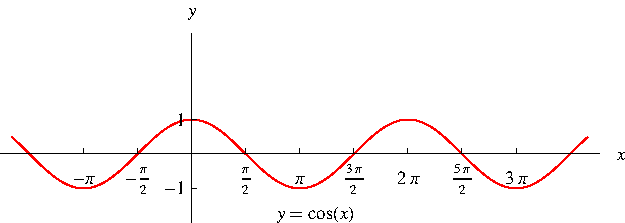
\includegraphics[width=12cm]{inverse-trig/pictures/07-06-arccosa.pdf}%
%}%
%\only<2>{%
%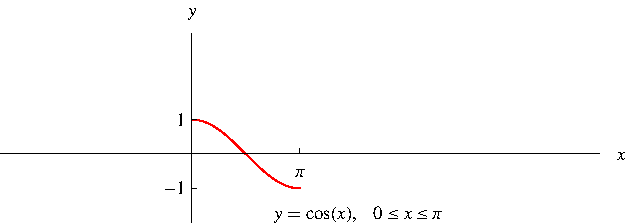
\includegraphics[width=12cm]{inverse-trig/pictures/07-06-arccosb.pdf}%
%}%
%\only<handout:0| 3->{%
%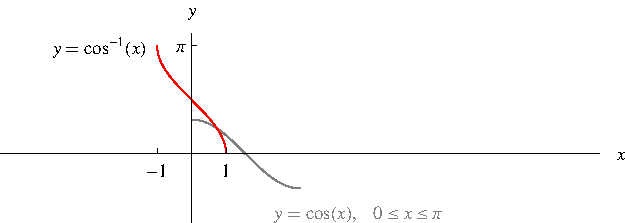
\includegraphics[width=12cm]{inverse-trig/pictures/07-06-arccosc.pdf}%
%}%
\psset{xunit=0.6cm,yunit=0.6cm}
\begin{pspicture}(-5,-1.4)(10,1.4)
\tiny
\psaxes[labels=none, ticks=x, Dx=1.570796327, Dy=1] {<->}(0,0)(-4,-1.4)(10,3.4)
\psLabels{10}{3.4}
\uncover<1>{\psplot[linecolor=red, plotpoints=1000]{-4}{10}{x 57.295779513 mul cos}
\rput[t](3.5, 1){$y=\cos x$}
}
\uncover<2>{\psplot[linecolor=red, plotpoints=1000]{0}{3.141592654}{x 57.295779513 mul cos}
\rput[t](3.5, 1){$y=\cos x, \quad 0\leq x\leq \pi$}
}
\uncover<3->{\psplot[linecolor=gray, plotpoints=1000]{0}{3.141592654}{x 57.295779513 mul cos}
\rput[t](3.5, 1){\color{gray}$y=\cos x, \quad 0\leq x\leq \pi$}

\psplot[linecolor=red, plotpoints=1000]{-1}{1}{x ACOS}
\psline(-0.1,3.141592654)(0.1,3.141592654)
\rput[l](0.15,3.141592654){$\pi$}
\psline(-1,-0.1)(-1,0.1)
\rput[t](-1,-0.1){$-1$}
\psline(1,-0.1)(1,0.1)
\rput[t](1,-0.1){$1$}
\rput[r](-0.6, 0.4){$y=\Arccos x$}
}

\rput[t](-3.14, -0.3){$-\pi$}
\rput[t](-1.57, -0.3){$-\frac{\pi}{2}$}
\rput[t](1.57, -0.3){$\frac{\pi}{2}$}
\rput[t](3.14, -0.3){$\pi$}
\rput[t](4.71, -0.3){$\frac{3\pi}{2}$}
\rput[t](6.28, -0.3){$2\pi$}
\rput[t](7.85, -0.3){$\frac{5\pi}{2}$}
\rput[t](9.42, -0.3){$3\pi$}
\rput[br](-0.2,1){\tiny $1$}

\end{pspicture}

\begin{columns}[c]
\column{.65\textwidth}
\begin{itemize}
\item<1->  Same for $\cos x$.
\item<2->  Restrict the domain to $[0, \pi ]$.
\item<3->  The inverse is called $\arccos$ or $\cos^{-1}$.
\item<5->  $\Arccos (x) = y \Leftrightarrow \cos y = x$ and $0 \leq y \leq \pi$.
\end{itemize}
\column{.35\textwidth}
\uncover<4->{%
%\uncover<4->{%
%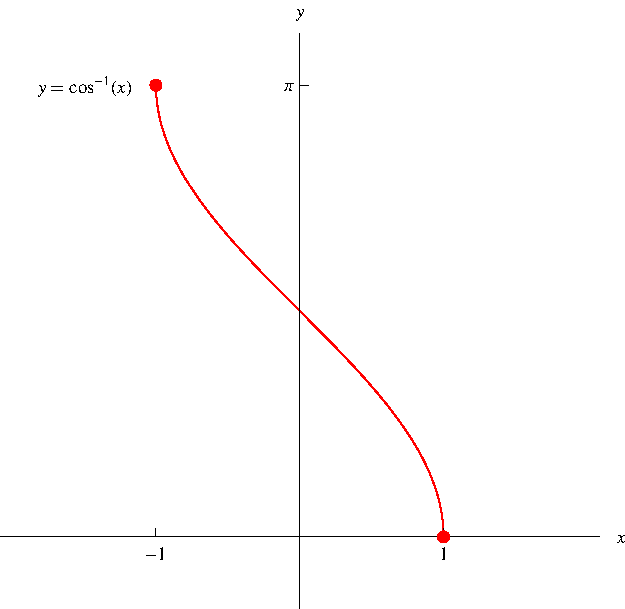
\includegraphics[height=4cm]{inverse-trig/pictures/07-06-arccosd.pdf}%
%}%
\psset{xunit=1.2cm,yunit=1.2cm}
\begin{pspicture}(-5,-1.4)(10,1.4)
\tiny
\psaxes[labels=none, ticks=none] {<->}(0,0)(-2,-0.5)(1.6,3.7)
\psLabels{1.6}{3.7}
\psplot[linecolor=red, plotpoints=1000]{-1}{1}{x ACOS}
\psline(-0.1,3.141592654)(0.1,3.141592654)
\rput[l](0.15,3.141592654){$\pi$}
\psline(-1,-0.1)(-1,0.1)
\rput[t](-1,-0.1){$-1$}
\psline(1,-0.1)(1,0.1)
\rput[t](1,-0.1){$1$}
\rput[r](-0.6, 2){$y=\Arccos x$}
\end{pspicture}
}%
\end{columns}
\end{frame}
% end module arccos-def


% begin module arccos-properties
\begin{frame}
Important facts about $\cos^{-1}$:
\begin{columns}[c]
\column{.5\textwidth}
\ 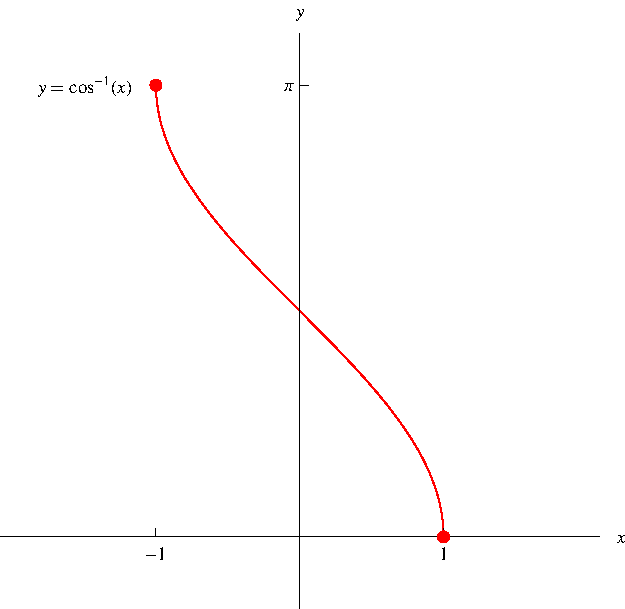
\includegraphics[height=6cm]{inverse-trig/pictures/07-06-arccosd.pdf}%
\column{.5\textwidth}
\begin{enumerate}
\item  \alert<handout:0| 2-3>{Domain: \uncover<3->{$[-1, 1]$.}}
\item  \alert<handout:0| 4-5>{Range: \uncover<5->{$[0, \pi ]$.}}
\item  $\cos^{-1} x = y \Leftrightarrow \cos y = x$ and $0 \leq y \leq \pi$.
\item  $\cos^{-1} (\cos x) = x$ for $0 \leq x \leq \pi$.
\item  $\cos (\cos^{-1} x) = x$ for $-1 \leq x \leq 1$.
\item  $\frac{\diff}{\diff x} (\cos^{-1} x) = -\frac{1}{\sqrt{1-x^2}}$.  \uncover<6->{(The proof is similar to the proof of the formula for the derivative of $\sin^{-1} x$.)}
\end{enumerate}
\end{columns}
\end{frame}
% end module arccos-properties

% begin module arctan-def
\begin{frame}
\begin{columns}[c]
\column{.5\textwidth}
\ \only<handout:0| -1>{%
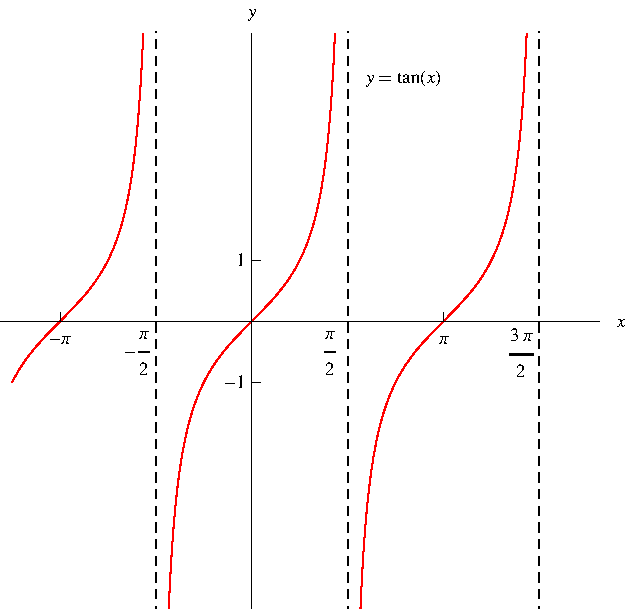
\includegraphics[width=5cm]{inverse-trig/pictures/07-06-arctana.pdf}%
}%
\only<handout:1| 2>{%
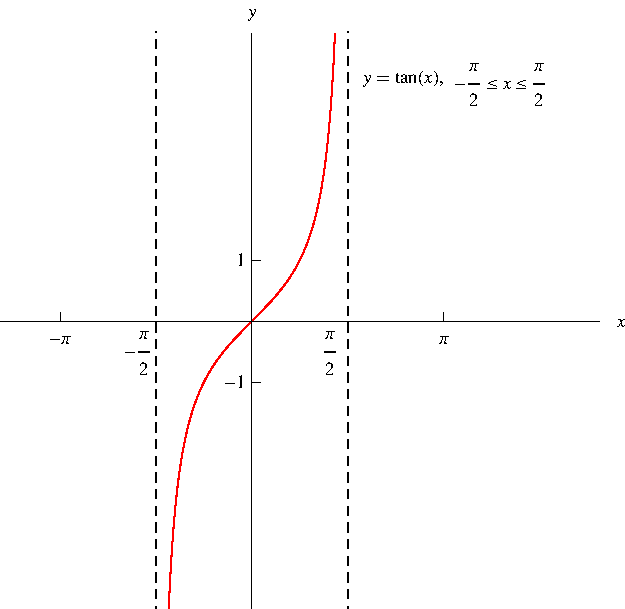
\includegraphics[width=5cm]{inverse-trig/pictures/07-06-arctanb.pdf}%
}%
\only<handout:2| 3->{%
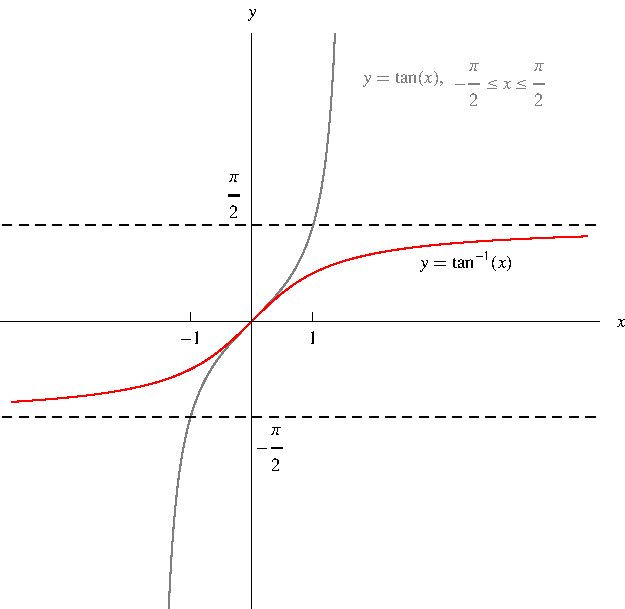
\includegraphics[width=5cm]{inverse-trig/pictures/07-06-arctanc.pdf}%
}%
\column{.5\textwidth}
\begin{itemize}
\item<1->  $\tan x$ isn't one-to-one.
\item<2->  Restrict the domain to $(-\pi /2, \pi /2)$.
\item<3->  The inverse is called $\Arctan$ or $\arctan$.
\item<4->  $\Arctan x = y \Leftrightarrow \tan y = x$ and $-\pi /2 < y < \pi /2$.
\item<5->  \alert<handout:0| 5-6>{Domain of $\Arctan$: \uncover<6-| handout:0>{$(-\infty,\infty)$.}}
\item<5->  \alert<handout:0| 7-8>{Range of $\Arctan$: \uncover<8-| handout:0>{$(-\pi / 2, \pi / 2)$.}}
\item<9->  \alert<handout:0| 9-10>{$\displaystyle \lim_{x\rightarrow \infty} \Arctan x = \uncover<10-| handout:0>{\pi / 2.}$}
\item<9->  \alert<handout:0| 11-12>{$\displaystyle \lim_{x\rightarrow - \infty} \Arctan x = \uncover<12-| handout:0>{- \pi / 2.}$}
\end{itemize}
\end{columns}
\end{frame}
% end module arctan-def

% begin module arctan-ex3
\begin{frame}
\begin{example}
Simplify the expression $\cos (\Arctan x)$.
\begin{itemize}
\item<2->  Let $y = \Arctan x$, so $\tan y = x$.
\item<3->  Draw a right triangle with opposite $x$ and adjacent $1$.
\item<4->  \alert<handout:0| 4-5>{Length of hypotenuse $ = \uncover<5->{\sqrt{1^2+x^2}.}$}
\item<6->  Then \alert<handout:0| 6-7>{$\cos (\Arctan x) = \uncover<7-| handout:0>{\frac{1}{\sqrt{1+x^2}}.}$}
\end{itemize}
\begin{pspicture}(-0.2,-0.5)(4.5,3.2)
\psframe*[linecolor=white](-0.2,-0.5)(4.5,3.2)
\psline[linecolor=red!1](4.5,-0.5)(4.5,-0.49)
\psline(0,0)(4,0)(4,3)(0,0)
\psline(3.8,0)(3.8,0.2)(4,0.2)
\fcAngle{0}{0.643501}{0.5}{$y$}
\uncover<3->{%
\rput[l](4.1, 1.5){$x$}
\rput[t](2,-0.1 ){\alertNoH{6,7}{$1$}}
}%
\uncover<5->{%
\rput[rb](1.9,1.6){\alertNoH{6,7}{$\sqrt{x^2+1}$}}
}%
\end{pspicture}
%\ \only<handout:0| -2>{%
%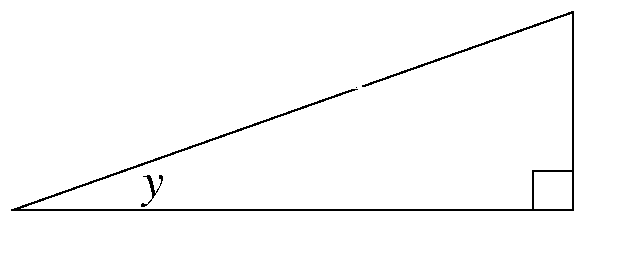
\includegraphics[width=5cm]{inverse-trig/pictures/07-06-ex3a.pdf}%
%}%
%\only<handout:0| 3-4>{%
%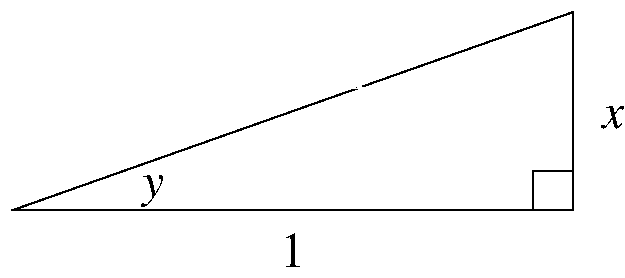
\includegraphics[width=5cm]{inverse-trig/pictures/07-06-ex3b.pdf}%
%}%
%\only<5->{%
%\includegraphics[width=5cm]{inverse-trig/pictures/07-06-ex3c.pdf}%
%}%
\end{example}
\end{frame}
% end module arctan-ex3

% begin module arctan-ex4
\begin{frame}
\begin{example}
Evaluate
\[
\lim_{x\rightarrow 2^+} \Arctan \left( \frac{1}{x-2}\right) .
\]
\uncover<2->{
\[
\frac{1}{x-2} \rightarrow \infty \qquad \text{ as } \qquad x\rightarrow 2^+.
\]
}
\uncover<3->{
Therefore
\[
\alertNoH{ 3-4}{\lim_{x\rightarrow 2^+} \Arctan \left( \frac{1}{x-2}\right) = \fcAnswer{4}{\worksheet{\frac{\pi}{2}}.}}
\]
}
\end{example}
\end{frame}
% end module arctan-ex4

% begin module arctan-derivative
\begin{frame}
\begin{theorem}[The Derivative of $\Arctan x$]
\[
\frac{\diff}{\diff x} (\Arctan x) = \frac{1}{1 + x^2}.
\]
\end{theorem}
\begin{proof}
\abovedisplayskip=0pt
\belowdisplayskip=-15pt
\abovedisplayshortskip=0pt
\belowdisplayshortskip=0pt
\begin{align*}
\uncover<2->{%
\text{Let}\quad y %
}%
& \uncover<2->{%
 = \Arctan x.
}\\%
\uncover<2->{%
\text{Then}\quad \alert<handout:0| 3-4,10>{\tan y} %
}%
& \uncover<2->{%
 \alert<handout:0| 10>{=}  \alert<handout:0| 5-6,10>{x.} %
}\\%
\uncover<3->{%
\text{Differentiate implicitly:}\quad \alert<handout:0| 3-4>{\uncover<4->{\sec^2 y \cdot y'}} %
}%
& \uncover<3->{%
 = \uncover<6->{\alert<handout:0| 6>{1}} 
}\\%
\uncover<7->{%
y' %
}%
& \uncover<7->{%
 = \frac{1}{\alert<handout:0| 8-9>{\sec^2 y}} %
}\\%
& \uncover<8->{%
 = \frac{1}{\alert<handout:0| 8-9>{\uncover<9->{1+\alert<handout:0| 10>{\tan^2 y}}}} %
}\\%
& \uncover<10->{%
 = \frac{1}{1+\alert<handout:0| 10>{x^2}}. \qedhere%
}%
\end{align*}
\end{proof}
\end{frame}
% end module arctan-derivative

% begin module inverse-trig-summary
\begin{frame}
The remaining inverse trigonometric functions aren't used often, and are summarized here.
\[
\begin{array}{llcrcl}
y = \csc^{-1} x &%
(|x| \geq 1) &%
\Leftrightarrow &%
\csc y = x &%
\text{ and } &%
y\in (0,\pi /2] \cup (\pi , 3\pi /2] \\%
y = \sec^{-1} x &%
(|x| \geq 1) &%
\Leftrightarrow &%
\sec y = x &%
\text{ and } &%
\alert<2>{y\in [0,\pi /2) \cup [\pi , 3\pi /2)} \\%
y = \cot^{-1} x &%
(|x| \in \mathbb{R}) &%
\Leftrightarrow &%
\cot y = x &%
\text{ and } &%
y\in (0,\pi )
\end{array}
\]

\ \only<handout:0| -1>{%
\includegraphics[width=5cm]{inverse-trig/pictures/07-06-seca.pdf}%
}%
\only<2->{%
\includegraphics[width=5cm]{inverse-trig/pictures/07-06-secb.pdf}%
}%
\end{frame}

\begin{frame}
Table of derivatives of inverse trigonometric functions: 
\begin{align*}
\frac{\diff}{\diff x} (\arcsin x) & = %
\frac{1}{\sqrt{1-x^2}} &%
\frac{\diff}{\diff x} (\csc^{-1} x) & = %
-\frac{1}{x\sqrt{x^2-1}} \\%
\frac{\diff}{\diff x} (\arccos x) & = %
-\frac{1}{\sqrt{1-x^2}} &%
\frac{\diff}{\diff x} (\sec^{-1} x) & = %
\frac{1}{x\sqrt{x^2-1}} \\%
\frac{\diff}{\diff x} (\arctan x) & = %
\frac{1}{1+x^2} &%
\frac{\diff}{\diff x} (\cot^{-1} x) & = %
-\frac{1}{1+x^2} %
\end{align*}
\end{frame}
% end module inverse-trig-summary

% begin module arcsin-ex5
\begin{frame}
\chainruley{\frac{1}{\sin^{-1}x}}{\sin^{-1} x}{u^{-1}}{-UU^{-2}}{\frac{1}{\sqrt{1-x^2}}}{-\frac{1}{(UU)^2\sqrt{1-x^2}}}{0}
\end{frame}
% end module arcsin-ex5

% end lecture

% begin lecture
\lect{March 21, 2014}{Lecture 16}{16}
\section{Sequences}
% begin module sequence-def-example
\begin{frame}
\begin{example}[A sequence]
\[
1, 2, 3, 4, 5, \ldots
\]
is an example of a sequence.  
\end{example}

\uncover<2->{%
\begin{definition}[Sequence, Terms]
A sequence is a list of numbers written in a definite order.  
The individual numbers in the sequence are called the terms of the sequence.  
\end{definition}
}%

\uncover<3->{%
\begin{example}[More sequences]
\begin{tabular}{rrrrrrcl}
$ 1,$ & $ 2,$ & $ 4,$ & $ 8,$ & $16,$ & $32,$ & $\ldots$ & is a sequence.  \\
$-1,$ & $ 1,$ & $-1,$ & $ 1,$ & $-1,$ & $ 1,$ & $\ldots$ & is a sequence.  \\
\uncover<4->{ $ 1,$ & $-1,$ & $ 1,$ & $-1,$ & $ 1,$ & $-1,$ & $\ldots$ & is a different sequence. }
\end{tabular}
\end{example}
}%

\end{frame}
% end module sequence-def-example

% begin module finite-sequence
\begin{frame}
\begin{example}[A finite sequence]
\[
1, 2, 3, 4, 5
\]
is an example of a finite sequence.  So is
\[
-1, -2, -3, \ldots , -10 000.
\]
\end{example}

\begin{definition}[Finite sequence, Infinite sequence]
A finite sequence is a sequence that ends.  
It is possible to write down all the terms in a finite sequence.  
A sequence that is not finite is called an infinite sequence.  
\end{definition}

\uncover<2->{%
\begin{example}[An infinite sequence]
\[
2, 4, 6, 8, \ldots
\]
is an example of an infinite sequence.  
\end{example}
}%

\end{frame}
% end module finite-sequence

% begin module notation
\begin{frame}
\begin{example}[Sequence notation]
Consider the sequence
\[
2, 4, 6, 8, \ldots.
\]
We can express this sequence more compactly using the notation
\[
a_n = 2n,
\]
where $a_n$ denotes the $n$th term.  
\begin{align*}
\text{So} \quad a_1 & = 2\cdot 1 = 2 \\
a_2 & = 2\cdot 2 = 4 \\
a_3 & = 2\cdot 3 = 6 \\
a_4 & = 2\cdot 4 = 8 \\
 & \vdots
\end{align*}
\end{example}

\end{frame}
% end module notation

% begin module notation-examples
\begin{frame}
\begin{example}
The sequence 
\[
\left( -1, 1, -1, 1, -1, 1, \ldots \right)
\]
can be written as $b_n = (-1)^n$.  
\end{example}

\uncover<2->{
\begin{example}
The sequence 
\[
\left( 1,2,4,8,16,\ldots\right)
\]
can be written as $c_n = 2^{n-1}$.  
\end{example}
}

\uncover<3->{
\begin{example}
The sequence 
\[
\left( \frac{1}{2}, -\frac{1}{4},\frac{1}{8},-\frac{1}{16},\ldots\right)
\]
can be written as $d_n = -\big( -\frac{1}{2}\big)^n$.  
\end{example}
}
\end{frame}
% end module notation-examples

% begin module find-terms
\begin{frame}
\begin{example}[Sequences via formulas: find sequence terms]
Find the first five terms of each of the following sequences.  
\begin{enumerate}
\item<alert@2-3| handout:alert@0>  $a_n = 3\cdot 2^{-n}$
\[
\uncover<3-| handout:0>{%
\frac{3}{2},\frac{3}{4},\frac{3}{8},\frac{3}{16},\frac{3}{32},\ldots
}%
\]
\item<alert@4-5| handout:alert@0>  $b_n = 1$
\[
\uncover<5-| handout:0>{%
1,1,1,1,1,\ldots
}%
\]
\item<alert@6-7| handout:alert@0>  $c_n = -3(n-1)+5$
\[
\uncover<7-| handout:0>{%
5,2,-1,-4,-7,\ldots
}%
\]
\item<alert@8-9| handout:alert@0>  $d_n = n^2+1$
\[
\uncover<9-| handout:0>{%
2,5,10,17,26,\ldots
}%
\]
\end{enumerate}
\end{example}

\end{frame}
% end module find-terms

% begin module find-formula
\begin{frame}
\begin{example}[Given the terms, find a formula]
Find a formula for the $n$th term of each of the following sequences.  
\begin{enumerate}
\item<alert@2-3>  $a_n = \uncover<3-| handout:0>{2\cdot \big(\frac{1}{4}\big)^n}$
\[
2, \frac{1}{2},\frac{1}{8},\frac{1}{32},\frac{1}{128},\ldots
\]
\item<alert@4-5>  $b_n = \uncover<5-| handout:0>{(-1)^nn^2}$
\[
-1,4,-9,16,-25,\ldots
\]
\item<alert@6-7>  $c_n = \uncover<7-| handout:0>{-1+6n}$
\[
-1,5,11,17,23,\ldots
\]
\end{enumerate}
\end{example}

\end{frame}
% end module find-formula

% begin module arithmetic-def
\begin{frame}
\begin{definition}[Arithmetic sequence]
An arithmetic sequence is one in which successive terms differ by a constant number.  
This constant is called the difference of the arithmetic sequence.  
\end{definition}

\begin{example}[Which are arithmetic?]
\begin{tabular}{rrrrrcl}
$ 1,$ & $ 2,$ & $ 3,$ & $ 4,$ & $ 5,$ & $\ldots$ & is arithmetic with difference $1$. \\
$23,$ & $16,$ & $ 9,$ & $ 2,$ & $-5,$ & $\ldots$ & is arithmetic with difference $-7$. \\
$ 8,$ & $ 9,$ & $12,$ & $17,$ & $24,$ & $\ldots$ & is not arithmetic. \\
& & & & & & $9-8=1$ but $12-9=3$.
\end{tabular}
\end{example}
\end{frame}
% end module arithmetic-def

% begin module arithmetic-ex
\begin{frame}
\begin{example}[Which are arithmetic?]
{\renewcommand{\arraystretch}{1.2}
\begin{tabular}{l|c|c|c|c}
Sequence & \alert<handout:0| 2-3,8-9,16-17>{Arithmetic?} & \alert<handout:0| 10-11,18-19>{Difference} & \alert<handout:0| 4-5,12-13,20-21>{First term} & \alert<handout:0| 6-7,14-15,22-23>{$n$th term} \\
\hline
\alert<handout:0| 2-7>{$1,-1,1,-1,\ldots$} & \uncover<3-| handout:0>{\alert<handout:0| 3>{no}} & \uncover<3-| handout:0>{\alert<handout:0| 3>{---}} & \uncover<5-| handout:0>{\alert<handout:0| 5>{$1$}} & \uncover<7-| handout:0>{\alert<handout:0| 7>{$(-1)^{n+1}$}} \\
\hline
\alert<handout:0| 8-15>{$\frac{1}{6},\frac{1}{2},\frac{5}{6},\frac{7}{6},\frac{3}{2},\ldots$} & \uncover<9-| handout:0>{\alert<handout:0| 9>{yes}} & \uncover<11-| handout:0>{\alert<handout:0| 11>{$\frac{1}{3}$}} & \uncover<13-| handout:0>{\alert<handout:0| 13>{$\frac{1}{6}$}} & \uncover<15-| handout:0>{\alert<handout:0| 15>{$\frac{1}{6}+\frac{1}{3}(n-1)$}} \\
\hline
\alert<handout:0| 16-23>{$2,2,2,2,\ldots$} & \uncover<17-| handout:0>{\alert<handout:0| 17>{yes}} & \uncover<19-| handout:0>{\alert<handout:0| 19>{$0$}} & \uncover<21-| handout:0>{\alert<handout:0| 21>{$2$}} & \uncover<23-| handout:0>{\alert<handout:0| 23>{$2\uncover<24->{\alert<handout:0| 24>{+0(n-1)}}$}} 
\end{tabular}
}%
\end{example}
\uncover<24->{%
If an arithmetic sequence has difference $d$, then the $n$th term has formula 
\[
a_n = a_1 + d(n-1),
\]
where $a_1$ is the first term.  
}%
\end{frame}
% end module arithmetic-ex

% begin module geometric-def
\begin{frame}
\begin{definition}[Geometric sequence]
A geometric sequence is one in which each term is obtained by multiplying the previous one by the same constant.  
This constant is called the ratio of the geometric sequence.  
\end{definition}

\begin{example}[Which are geometric?]
\begin{tabular}{rrrrrcl}
$  2,$ & $  4,$ & $  8,$ & $ 16,$ & $ 32,$ & $\ldots$ & is geometric with ratio $2$. \\
$  1,$ & $ -3,$ & $  9,$ & $-27,$ & $ 81,$ & $\ldots$ & is geometric with ratio $-3$. \\
$-42,$ & $-14,$ & $-21,$ & $ 31,$ & $-22,$ & $\ldots$ & is not geometric. \\
& & & & & & ($\frac{-14}{-42} = \frac{1}{3}$ but $\frac{-21}{-14} = \frac{3}{2}$.)
\end{tabular}
\end{example}
\end{frame}
% end module geometric-def

% begin module geometric-ex
\begin{frame}
\begin{example}[Arithmetic and geometric]
{\renewcommand{\arraystretch}{1.2}
\begin{tabular}{l|c|c|c|c|c}
& \alert<handout:0| 2-3,10-11,18-19,28-29,36-37>{Arithmetic/} &  &  &  & \\
Sequence & \alert<handout:0| 2-3,10-11,18-19,28-29,36-37>{geometric} & \alert<handout:0| 12-13,20-21>{Diff.} & \alert<handout:0| 4-5,22-23,30-31>{Ratio} & \alert<handout:0| 6-7,14-15,24-25,32-33,38-39>{$a_1$} & \alert<handout:0| 8-9,16-17,26-27,34-35,40-41>{$a_n$} \\
\hline
\alert<handout:0| 2-9>{$\frac{2}{3},\frac{4}{9},\frac{8}{27},\frac{16}{81},\ldots$} & \uncover<3-| handout:0>{\alert<handout:0| 3>{geometric}} & \uncover<3-| handout:0>{\alert<handout:0| 3>{---}} & \uncover<5-| handout:0>{\alert<5| handout:0>{$\frac{2}{3}$}} & \uncover<7-| handout:0>{\alert<handout:0| 7>{$\frac{2}{3}$}} & \uncover<9-| handout:0>{\alert<handout:0| 9>{$\big(\frac{2}{3}\big)^{n}\uncover<handout:0| 42->{\alert<handout:0| 42>{ = \frac{2}{3}\big(\frac{2}{3}\big)^{n-1}}}$}} \\
\hline
\alert<handout:0| 10-17>{$7,3,-1,-5,\ldots$} & \uncover<11-| handout:0>{\alert<handout:0| 11>{arithmetic}} & \uncover<13-| handout:0>{\alert<handout:0| 13>{$-4$}} & \uncover<11-| handout:0>{\alert<11| handout:0>{---}} & \uncover<15-| handout:0>{\alert<handout:0| 15>{$7$}} & \uncover<17-| handout:0>{\alert<handout:0| 17>{$7-4n$}} \\
\hline
\alert<handout:0| 18-27>{$4,4,4,4,\ldots$} & \uncover<19-| handout:0>{\alert<handout:0| 19>{both}} & \uncover<21-| handout:0>{\alert<handout:0| 21>{$0$}} & \uncover<23-| handout:0>{\alert<23| handout:0>{$1$}} & \uncover<25-| handout:0>{\alert<handout:0| 25>{$4$}} & \uncover<27-| handout:0>{\alert<handout:0| 27>{$4\uncover<handout:0| 42->{\alert<handout:0| 42>{ = 4(1)^{n-1}}}$}} \\
\hline
\alert<handout:0| 28-35>{$\pi,-\pi^2,\pi^3,-\pi^4,\ldots$} & \uncover<29-| handout:0>{\alert<handout:0| 29>{geometric}} & \uncover<29-| handout:0>{\alert<handout:0| 29>{---}} & \uncover<31-| handout:0>{\alert<31| handout:0>{$-\pi$}} & \uncover<33-| handout:0>{\alert<handout:0| 33>{$\pi$}} & \uncover<35-| handout:0>{\alert<handout:0| 35>{$\pi(-\pi)^{n-1}$}} \\
\hline
\alert<handout:0| 36-41>{$1,1,2,2,3,3,\ldots$} & \uncover<37-| handout:0>{\alert<handout:0| 37>{neither}} & \uncover<37-| handout:0>{\alert<handout:0| 37>{---}} & \uncover<37-| handout:0>{\alert<37| handout:0>{---}} & \uncover<39-| handout:0>{\alert<handout:0| 39>{$1$}} & \uncover<41-| handout:0>{\alert<handout:0| 41>{$\lceil\frac{n}{2}\rceil$}} \\
\end{tabular}
}%
\end{example}

\uncover<42->{%
If a geometric sequence has ratio $r$, then the $n$th term has formula 
\[
a_n = a_1r^{n-1}.
\]
where $a_1$ is the first term.  
}%
\end{frame}
% end module geometric-ex

% begin module sequence-ex2
\begin{frame}
Not all sequences can be represented by a simple formula.
\begin{example}[Example 2, p. 712]
\begin{enumerate}
\item  Consider the sequence $\{ p_n\}$, where $p_n$ is the population of the world as of January 1 of year $n$.  This has no simple formula.
\item<2->  Let $a_n$ be the $n$th digit of the number $e$.  Then the first few terms of $\{ a_n\}$ are
\uncover<2->{%
\[
\{ 7, 1, 8, 2, 8, 1, 8, 2, 8, 4, 5, \ldots \}
\]
}%
\item<3->  The Fibonacci sequence $\{ f_n\}$ is defined recursively by
\[
f_1 = 1 \qquad f_2 = 1 \qquad f_n = f_{n-1} + f_{n-2}, \quad n\geq 3
\]
\uncover<4->{%
The first few terms are
\abovedisplayskip=1pt
\belowdisplayskip=1pt
\[
\{%
\alert<handout:0| 4-5>{1},%
\alert<handout:0| 4-7>{1},%
\uncover<5->{\alert<handout:0| 5-9>{{2},}}%
\uncover<7->{\alert<handout:0| 7-11>{{3},}}%
\uncover<9->{\alert<handout:0| 9-13>{{5},}}%
\uncover<11->{\alert<handout:0| 11-13>{{8},}}%
\uncover<13->{\alert<handout:0| 13>{{13},\ldots }}%
\}%
\]
}%
\uncover<14->{%
The Fibonacci sequence can be described by a formula, but not a simple one.%
}%
\end{enumerate}
\end{example}
\end{frame}
% end module sequence-ex2

% end lecture

% begin lecture
\lect{March 28, 2014}{Lecture 18}{18}
\section{Series}
% begin module series-def-example
\begin{frame}
\begin{example}[A series]
\[
1 + 2 + 3 + 4 + 5
\]
is an example of a series.  
\end{example}

\uncover<2->{%
\begin{definition}[Series, Sum]
A series is what you get if you add together the terms of a sequence.  
The sum of a series is the number that results from adding up its terms.  
Some series do not have a sum.  
\end{definition}
}%

\uncover<3->{%
\begin{example}[A series with a sum]
The sum of the series %
$1 + 2 + 3 + 4 + 5$ %
is \uncover<4-| handout:0>{15.} 
\end{example}
}%

\uncover<5->{%
\begin{example}[A series with no sum]
The series %
$1 + 2 + 3 + 4 + 5 + \cdots $ %
has no sum.  
\end{example}
}%

\end{frame}
% end module series-def-example

% begin module finite-series
\begin{frame}
\begin{example}[A finite series]
\[
1 + 2 + 3 + 4 + 5
\]
is an example of a finite series.  So is
\[
-1 - 2 - 3 - \ldots - 10 000.
\]
\end{example}

\begin{definition}[Finite series, Infinite series]
A finite series is a series that ends.  
It is possible to write down all the terms in a finite series.  
A series that is not finite is called an infinite series.  

Every finite series has a sum.  
Some infinite series have a sum, and others do not.  
\end{definition}

\uncover<2->{%
\begin{example}[An infinite series]
\[
1 + 1 + 1 + 1 + \ldots
\]
is an example of an infinite series.  
It has no sum.  
\end{example}
}%

\end{frame}
% end module finite-series

% begin module arithmetic-sum
\begin{frame}
\begin{definition}[Arithmetic series]
An arithmetic series is a series whose terms are an arithmetic sequence.
\end{definition}

\begin{example}[Sum of a small arithmetic series]
The sum of the arithmetic series %
$7 + 4 + 1 - 2 - 5$ %
is \uncover<2-| handout:0>{\alertNoH{ 2}{5}.}
\end{example}

\uncover<3->{%
\begin{example}[Sum of a large arithmetic series]
Find the sum of the arithmetic series
\abovedisplayskip=0pt
\belowdisplayskip=0pt
\[
7 + 4 + 1 - 2 - 5 - \cdots - 53 - 56.
\]
\uncover<4->{Let $s$ denote the sum.}
\uncover<5->{%
\abovedisplayskip=2pt
\belowdisplayskip=2pt
\[
\begin{array}{rcrrrrr}
s & = & \alertNoH{ 7-8}{7} & \alertNoH{ 9-10}{+ 4} & \alertNoH{ 11-12}{+ 1} & - \cdots & \alertNoH{ 13-14}{- 56} \\
\uncover<7->{+}\uncover<6->{s} & \uncover<6->{=} & \uncover<6->{\alertNoH{ 7-8}{-56}} & \uncover<6->{\alertNoH{ 9-10}{-53}} & \uncover<6->{\alertNoH{ 11-12}{-50}} & \uncover<6->{- \cdots} & \uncover<6->{\alertNoH{ 13-14}{+ 7}} \\
\hline
\uncover<7->{2s} & \uncover<7->{=} & \uncover<8->{\alertNoH{ 8}{-49}} &\uncover<10->{\alertNoH{ 10}{-49}} &\uncover<12->{\alertNoH{ 12}{-49}} & \uncover<13->{-\cdots} & \uncover<14->{\alertNoH{ 14}{-49}}
\end{array}
\]
}%

\vspace{-12pt}
\abovedisplayskip=2pt
\belowdisplayskip=2pt
\begin{align*}
\uncover<15->{\text{Therefore}\quad 2s & = (-49)\alertNoH{ 15-16}{(\uncover<16->{22})}} \\
\uncover<17->{s & = -49\cdot 22/2 = -539.}
\end{align*}
\end{example}
}%

\end{frame}
% end module arithmetic-sum

% begin module arithmetic-sum-theorem
\begin{frame}
\begin{theorem}[Sum of an arithmetic series]
The sum of a finite arithmetic series is the average of the first and last terms, multiplied by the number of terms.  
That is,
\[
a + (a + d) + (a + 2d) + \cdots + (a + (n-1)d) = \frac{a + (a+(n-1)d)}{2}n.
\]
The only infinite arithmetic series with a sum is the series of all $0$.
\end{theorem}

\uncover<2->{%
\begin{example}[Sum of an arithmetic series]
Find the sum of the arithmetic series
\[
5 + 10 + 15 + 20 + \cdots + 100.
\]
\uncover<3->{\alert<3-4| handout:0>{%
The series contains \uncover<4-| handout:0>{20} terms.  
}}%
\uncover<5->{%
The average of the first and last terms is \uncover<5-| handout:0>{$\frac{5+100}{2}$}.  
}%

\uncover<6->{%
Therefore the sum is $\frac{\uncover<6-| handout:0>{5+100}}{2} \cdot  \uncover<6-| handout:0>{20}   \uncover<handout:0|6->{=105\cdot 10 = 1050.}$
}%
\end{example}
}%

\end{frame}
% end module arithmetic-sum-theorem

% begin module notation
\begin{frame}
\begin{example}[Sequence notation]
Consider the sequence
\[
2, 4, 6, 8, \ldots.
\]
We can express this sequence more compactly using the notation
\[
a_n = 2n,
\]
where $a_n$ denotes the $n$th term.  
\begin{align*}
\text{So} \quad a_1 & = 2\cdot 1 = 2 \\
a_2 & = 2\cdot 2 = 4 \\
a_3 & = 2\cdot 3 = 6 \\
a_4 & = 2\cdot 4 = 8 \\
 & \vdots
\end{align*}
\end{example}

\end{frame}
% end module notation

% begin module geometric-sum
\begin{frame}
\begin{definition}[Geometric series]
A geometric series is a series whose terms are a geometric sequence.  
\end{definition}
\uncover<2->{%
\begin{example}[The sum of a finite geometric series]
Find the sum of the geometric series
\abovedisplayskip=2pt
\belowdisplayskip=2pt
\[
a + ar + ar^2 + ar^3 + \cdots + ar^{M-1} = \sum_{n = 1}^M ar^{n-1}.
\]
\uncover<3->{Let $s$ denote the sum.  }
\uncover<4->{%
\abovedisplayskip=2pt
\belowdisplayskip=2pt
\[
\begin{array}{rcrrrrrr}
\alert<handout:0| 6-7>{s} & = & \alert<handout:0| 8>{a} & + ar & + ar^2 & + \cdots & + ar^{M-1} & \\
\alert<handout:0| 6-7>{\uncover<6->{-}\qquad \uncover<5->{rs}} & \uncover<5->{=} &  &  \uncover<5->{ar} & \uncover<5->{+ ar^2} & \uncover<5->{+ \cdots} & \uncover<5->{+ ar^{n-1}} & \uncover<5->{+ \alert<handout:0| 8>{ar^M}}\\
\hline
\uncover<7->{\alert<handout:0| 7>{s - rs}} & \uncover<6->{=} & \multicolumn{6}{l}{\uncover<8->{\alert<handout:0| 8>{a-ar^M}}}\\
\uncover<9->{s} & \uncover<9->{=} & \multicolumn{6}{l}{\uncover<9->{\frac{a(1-r^M)}{1-r}}}
\end{array}
\]
}%

\end{example}
}%
\uncover<10->{%
\begin{theorem}[The sum of a finite geometric series]
The sum of the finite geometric series $\sum_{n=1}^M ar^{n-1}$ is $a\frac{1-r^M}{1-r}$.  
\end{theorem}
}%
\end{frame}
% end module geometric-sum

% begin module geometric-sum-example
\begin{frame}
\begin{example}[The sum of a geometric series]
Find the sum of the geometric series
\abovedisplayskip=0pt
\belowdisplayskip=0pt
\[
\sum_{n=1}^{12} 6(-2)^{n-1}.
\]
\uncover<2->{%
\begin{align*}
\alert<handout:0| 2-3>{\text{The first term is } a} & \alert<handout:0| 2-3>{= \uncover<3-| handout:0>{6.}} \\
\alert<handout:0| 4-5>{\text{The ratio is } r} & \alert<handout:0| 4-5>{= \uncover<5-| handout:0>{-2.}} \\
\alert<handout:0| 6-7>{\text{The number of terms is } M} & \alert<handout:0| 6-7>{= \uncover<7-| handout:0>{12.}} \\
\alert<handout:0| 8-9>{\text{The sum is } s} & \alert<handout:0| 8-9>{= \uncover<9-| handout:0>{6\frac{1-(-2)^{12}}{1-(-2)} = -8190.}} 
\end{align*}
}%
\end{example}

\end{frame}
% end module geometric-sum-example

% begin module geometric-sum-example
\begin{frame}

\begin{example}[A geometric series in non-standard form]
Find the sum of the geometric series
\abovedisplayskip=0pt
\belowdisplayskip=0pt
\[
\sum_{n=1}^{7} \frac{1}{2^{2n+1}}.
\]
\uncover<2->{%
\begin{align*}
\alert<handout:0| 2-3>{\text{The first term is } a} & \alert<handout:0| 2-3>{= \uncover<3-| handout:0>{\frac{1}{8}.}} \\
\alert<handout:0| 4-5>{\text{The ratio is } r} & \alert<handout:0| 4-5>{= \uncover<5-| handout:0>{\frac{1}{4}.}} \\
\alert<handout:0| 6-7>{\text{The number of terms is } M} & \alert<handout:0| 6-7>{= \uncover<7-| handout:0>{7.}} \\
\alert<handout:0| 8-9>{\text{The sum is } s} & \alert<handout:0| 8-9>{= \uncover<9-| handout:0>{\frac{1}{8}\frac{1-\big(\frac{1}{4}\big)^7}{1-\big(\frac{1}{4}\big)} \approx 0.1667.}}
\end{align*}
}%
\end{example}

\end{frame}
% end module geometric-sum-example

% begin module arithmetic-sum-indices
\begin{frame}
The indices in series notation don't always start at $n = 1$.
\begin{example}[Different starting index]
Find the sum of the series
\abovedisplayskip=0pt
\belowdisplayskip=0pt
\[
\sum_{n=3}^{14} 4 + \frac{n}{2}.
\]
\alertNoH{ 2-3}{\uncover<2->{This series is \uncover<3->{arithmetic.}}}
\uncover<4->{%
\begin{align*}
\alertNoH{ 4-5}{\text{The first term is } a_3} & \alertNoH{ 4-5}{= \uncover<5-| handout:0>{4+\frac{3}{2}=\frac{11}{2}.}} \\
\alertNoH{ 6-7}{\text{The last term is } a_{14}} & \alertNoH{ 6-7}{= \uncover<7-| handout:0>{4+\frac{14}{2}=11.}} \\
\alertNoH{ 8-9}{\text{The number of terms is } M} & \alertNoH{ 8-9}{= \uncover<9-| handout:0>{12.}} \\
\alertNoH{ 10-11}{\text{The sum is } s} & \alertNoH{ 10-11}{= \uncover<11-| handout:0>{\frac{11/2+11}{2}\cdot 12 = \frac{33}{4}\cdot 12 = 99.}}
\end{align*}
}%
\end{example}

\end{frame}
% end module arithmetic-sum-indices

% begin module infinite-geometric
\begin{frame}
Sometimes an infinite geometric series has a sum.  

The formula for the sum of a geometric series with first term $a$, ratio $r$, and $M$ terms is
\[
a\frac{1-r^M}{1-r}.
\]
If $r$ is less than $1$ in modulus, then $r^M\to 0$ as $M\to\infty$, so the sum goes to $a\frac{1}{1-r}$ as $M$ gets bigger.  Therefore
\[
\sum_{n=1}^\infty  ar^{n-1} = a\frac{1}{1-r} \quad \text{if}\quad |r|<1.
\]
If $r$ is bigger than or equal to $1$ in modulus, then $r^M$ increases without bound, so
\[
\sum_{n=1}^\infty  ar^{n-1}  \quad \text{does not exist if } |r|\geq 1.
\]
\end{frame}
% end module infinite-geometric

% begin module infinite-geometric-example
\begin{frame}
\begin{example}[The sum of an infinite geometric series]
Find the sum of the geometric series
\abovedisplayskip=0pt
\belowdisplayskip=0pt
\[
\sum_{n=1}^{\infty} \frac{1}{2^n}.
\]
\uncover<2->{%
\begin{align*}
\alert<handout:0| 2-3>{\text{The ratio is } r} & \alert<handout:0| 2-3>{= \uncover<3-| handout:0>{\frac{1}{2}.}} \\
\alert<handout:0| 4-5>{ |r|} & \alert<handout:0| 4-5>{\uncover<5-| handout:0>{<}1.} \\
\alert<handout:0| 6-7>{\text{The first term is } a} & \alert<handout:0| 6-7>{= \uncover<7-| handout:0>{\frac{1}{2}.}} \\
\alert<handout:0| 8-9>{\text{The sum is } s} & \alert<handout:0| 8-9>{= \uncover<9-| handout:0>{\frac{1}{2}\cdot\frac{1}{1-\frac{1}{2}} = 1.}}
\end{align*}
}%
\end{example}

\end{frame}
% end module infinite-geometric-example

% end lecture

\end{document}
